
\documentclass[a4paper,12pt]{report}
\usepackage{a4wide}

%\documentclass[a5paper,10pt]{book}
%\usepackage[top=23mm, bottom=18mm, left=15mm, right=25mm]{geometry}
%\geometry{papersize={170mm,220mm}}


\usepackage[utf8x]{inputenc}
\usepackage[danish]{babel}

\usepackage{xr-hyper} %Externe hyper-ref
\usepackage[colorlinks=true, hyperindex=true, linkcolor=minmblaa, citecolor=minmblaa, urlcolor=minmblaa]{hyperref}
\hypersetup{colorlinks=true,filecolor=minmblaa,bookmarksnumbered=true} %Til hyperreferencer. Referencer med farver
\usepackage{needspace} % giver mulighed for at kræve at der skal være et antal tomme linier på siden før ellers indsættes et sideskift.
\usepackage{framed} %Bokse
\usepackage{wrapfig}

\usepackage{amsmath,amsfonts,amssymb,amsthm,mathtools} %Matematikpakker

\setlength{\parindent}{0mm} %Ingen Indhak i første linje i afsnit

\usepackage{color} %Farvepakke

\usepackage{array}
\usepackage{colortbl}
\usepackage{multirow} %Til at flette rækker i tabeller.

\usepackage{verbatim,mhchem}



	% DOWNLOAD FRA: http://sarovar.org/frs/?group_id=52&release_id=97
	% Læg i directory for hoved TEX fil
%\usepackage[draft]{pdfdraftcopy}
%\draftstring{Licens: Kasper Langt Mellemnavn Skårhøj}
%\draftfontsize{30}
	%\draftfontfamily{hlh}
	%\draftangle{45}
	%\definecolor{mycolor}{rgb}{.825,.855,1}
	%\draftcolor{mycolor}
	%\draftfontattrib



% = Sidehoved =
\usepackage{fancyhdr}
\pagestyle{fancy}
\renewcommand{\sectionmark}[1]{\markright{\protect\titlegraphic{dturoed}\textcolor{dtugraa}{\thesection~\MakeUppercase{#1}}}} % \thesection.\
\fancyhead{}
\fancyfoot{}
\fancyhead[R]{\titlefont\thepage}
\fancyhead[C]{}
\fancyhead[L]{\titlefont \small eNote \MakeUppercase{~\thechapter}~\hspace*{1ex}\rightmark}
\renewcommand\headrulewidth{0pt}
\fancypagestyle{plain}{\fancyfoot[C]{}}% {\titlefont\footnotesize\thepage}}
\setlength{\headheight}{15pt}


% = Længder
%\newlength{\envtblsep}\setlength{\envtblsep}{1\FrameSep}
\newlength{\obsl}\setlength{\obsl}{\textwidth-1.2cm-13.2pt}

% Includes:

% =     Fonts (select one)    =
\usepackage{mathpazo}\linespread{1.05} % Palatino needs more leading (space between lines)
\usepackage{bm} % bold math, must be loaded after the fontpackages

% % Til overskrifter
\DeclareTextFontCommand{\th}{\fontencoding{T1}\fontfamily{phv}\fontseries{b}\selectfont}
\newcommand\titlefont{\fontencoding{T1}\fontfamily{phv}\selectfont}


% =     PGF grafik      =
\usepackage{tikz}
\newcommand\titlegraphic[1]{%
\tikz[baseline] %
\draw[thick,color=#1]
(0pt  ,-0.25em) -- (0pt  ,0.85em)
(2.5pt,-0.25em) -- (2.5pt,0.85em)
(5pt  ,-0.25em) -- (5pt  ,0.85em)
(7.5pt,-0.25em) -- (7.5pt,0.85em);\hspace*{0.8ex} %
}

\newcommand\titlegraphicwide[1]{%
\tikz[baseline] %
\draw[line width=0.8mm,color=#1]
(0pt  ,-0.25em) -- (0pt  ,0.85em)
(4.5pt,-0.25em) -- (4.5pt,0.85em)
(9pt  ,-0.25em) -- (9pt  ,0.85em)
(13.5pt,-0.25em) -- (13.5pt,0.85em);\hspace*{0.8ex} %
}


% =      Title Layout      =
\usepackage{titlesec}
\makeatletter
\titleformat{\chapter}
	[display] % Shape
	{\titlefont\Huge\flushleft} % Title and label format
	{\titlefont\LARGE\bfseries \titlegraphicwide{dturoed}\textcolor{dtugraa}{\@chapapp~\thechapter}} % label
	{0.9em} % label/title separation
	{} % before code
	[] % after code
\makeatother
\titleformat{\section}
	[hang] % Shape
	{\titlefont\Large\flushleft} % Title and label format
	{\thesection} % label
	{0.9em} % label/title separation
	{} % before code
	[] % after code
\titleformat{\subsection}
	[hang] % Shape
	{\titlefont\large} % Title and label format
	{\thesubsection} % label
	{0.9em} % label/title separation
	{} % before code
	[] % after code
\titlespacing{\subsection}{0pt}{*6}{*1.5}
\titleformat{\subsubsection}
	[hang] % Shape
	{\titlefont} % Title and label format
	{\thesubsubsection} % label
	{0.9em} % label/title separation
	{} % before code
	[] % after code



% = Farver
\definecolor{dturoed}{rgb}{0.6, 0.0, 0.0}
\definecolor{dtugraa}{rgb}{0.5, 0.5, 0.5}	% Lidt mørkere. Korrekt = 0.4
\definecolor{mingroenstreg}{rgb}{0.4,0.8,0}	% Sekundærfarve 14 : 102/204/0	(Forårsgrøn) -> Eksempler
\definecolor{mingroen}{rgb}{0.32,0.64,0}		% Sekundærfarve 14, 80% mørkere (tekst)
\definecolor{minorangestreg}{rgb}{1,0.6,0}		% Sekundærfarve 1 : 255/153/0	(Orange) -> Opgaver
\definecolor{minorange}{rgb}{0.8,0.48,0}		% Sekundærfarve 1 , 80% mørkere (tekst)

\definecolor{minblaa}{rgb}{0.2,0.4,0.8}	% Sekundærfarve 13 , 51/102/204 	( Blå -> Definitioner etc)
\definecolor{minmblaa}{rgb}{0.16,0.32,0.64}	% Sekundærfarve 13 , 80% mørkere (tekst)
\definecolor{thmbackground}{rgb}{0.97,.97, 0.99}	% Farve 13 - lys baggrund

\definecolor{mingraastreg}{rgb}{.5,.5,.5}
\definecolor{hvadbackground}{rgb}{0.97,.97, 0.97}
\definecolor{sumgul}{rgb}{1,1,.8}

\definecolor{hjmopgfarve}{rgb}{.96,1,.96}


% = Counter
\newcounter{evncount}[chapter]
\setcounter{evncount}{0}
\renewcommand{\theevncount}{\thechapter.\arabic{evncount}}
\renewcommand{\theequation}{\thechapter-\arabic{equation}}


% = Eksempler = example =
\newenvironment{example}[1][]{
	\refstepcounter{evncount}
	\setlength{\obsl}{\textwidth-1.2cm-13.2pt-9pt} % fix width of the info envirnment%
	\def\FrameCommand{ 
		\textcolor{mingroenstreg}{\vrule width 4pt} 
		\hspace{5pt} 
	}%
	\MakeFramed{\advance\hsize-\width \FrameRestore}%
	\needspace{3\baselineskip}
	\titlegraphic{mingroen}
	\textcolor{mingroen}{
		\th{Eksempel \theevncount \hspace*{5mm} #1}
	} 
	\vspace*{3mm}%
	\begin{small}
	\par
}
{
	\end{small}
	\endMakeFramed
}


% = Opgaver = exercise =
\newenvironment{exercise}[1][]{
	\refstepcounter{evncount}
	\setlength{\obsl}{\textwidth-1.2cm-13.2pt-9pt}% fix width of the info envirnment%
	\def\FrameCommand{
		\textcolor{minorangestreg}{\vrule width 4pt}
		\hspace{5pt}
	}%
	\MakeFramed{\advance\hsize-\width \FrameRestore}%
	\needspace{3\baselineskip}
	\titlegraphic{minorange}
	\textcolor{minorange}{
		\th{Opgave \theevncount \hspace*{5mm} #1}
	} 
	\vspace*{3mm}%
	\begin{small}
	\par
}
{
	\end{small}
	\endMakeFramed
}


% = Bevis
\newenvironment{bevis}{
	\setlength{\obsl}{\textwidth-1.2cm-13.2pt-9pt} % fix width of the info envirnment%
	\def\FrameCommand{
		\textcolor{mingraastreg}{\vrule width 4pt} 
		\hspace{5pt}
	}%
	\MakeFramed{\advance\hsize-\width \FrameRestore}%
	\needspace{3\baselineskip}
	\titlegraphic{black}
	\textcolor{black}{
		\th{Bevis}
	}
	\vspace*{3mm}%
	\begin{small}
	\par
}
{
	\bevisslut 
	\end{small}
	\endMakeFramed
}


% = Definition =
\newenvironment{definition}[1][]{
	\vspace{4mm}
	\pagebreak[1]
	\setlength{\obsl}{\textwidth-1.2cm-2\FrameSep-13.2pt}%
	\def\FrameCommand{
		\fboxsep=\FrameSep\fcolorbox{minblaa}{thmbackground}
	}
	\begin{minipage}{\textwidth}
	\MakeFramed{\advance\hsize-\width\FrameRestore}
	\refstepcounter{evncount}
	\titlegraphic{minblaa}
	\textcolor{minmblaa}{
		\th{Definition \theevncount \hspace*{5mm} #1}
	}
	\vspace*{3mm}
	\par
}
{
	\endMakeFramed 
	\end{minipage}
	\vspace{4mm}
}


% = Theorem =
\newenvironment{theorem}[1][]{
	\vspace{4mm}
	\pagebreak[1]%
	\setlength{\obsl}{\textwidth-1.2cm-2\FrameSep-13.2pt}%
	\def\FrameCommand{
		\fboxsep=\FrameSep\fcolorbox{minblaa}{thmbackground}
	}%
	\begin{minipage}{\textwidth}
	\MakeFramed{\advance\hsize-\width\FrameRestore}%
	\refstepcounter{evncount}
	\titlegraphic{minblaa}
	\textcolor{minmblaa}{
		\th{Sætning \theevncount \hspace*{5mm} #1}
	}
	\vspace*{3mm}
	\par
}
{
	\endMakeFramed 
	\end{minipage}
	\vspace{4mm}
}


% = Lemma =
\newenvironment{lemma}[1][]{
	\vspace{4mm}
	\pagebreak[1]
	\setlength{\obsl}{\textwidth-1.2cm-2\FrameSep-13.2pt}%
	\def\FrameCommand{
		\fboxsep=\FrameSep \fcolorbox{minblaa}{thmbackground}
	}
	\begin{minipage}{\textwidth} 
	\MakeFramed{\advance\hsize-\width \FrameRestore}
	\refstepcounter{evncount}
	\titlegraphic{minblaa}
	\textcolor{minmblaa}{
		\th{Hjælpesætning \theevncount \hspace*{5mm} #1}
	}
	\vspace*{3mm}
	\par
}
{
	\endMakeFramed 
	\end{minipage}
	\vspace{4mm}
}


% = Corollary =
\newenvironment{corollary}[1][]{
	\vspace{4mm}
	\pagebreak[1]
	\setlength{\obsl}{\textwidth-1.2cm-2\FrameSep-13.2pt}%
	\def\FrameCommand{
		\fboxsep=\FrameSep \fcolorbox{minblaa}{thmbackground}
	}
	\begin{minipage}{\textwidth} 
	\MakeFramed{\advance\hsize-\width \FrameRestore}
	\refstepcounter{evncount}
	\titlegraphic{minblaa}
	\textcolor{minmblaa}{
		\th{Følgesætning \theevncount \hspace*{5mm} #1}
	}
	\vspace*{3mm}
	\par
}
{
	\endMakeFramed 
	\end{minipage}
	\vspace{4mm}
}


% = Metode = method
\newenvironment{method}[1][]{
	\vspace{4mm}
	\pagebreak[1]
	\setlength{\obsl}{\textwidth-1.2cm-2\FrameSep-13.2pt}%
	\def\FrameCommand{
		\fboxsep=\FrameSep \fcolorbox{black}{hvadbackground}
	}
	\begin{minipage}{\textwidth} 
	\MakeFramed{\advance\hsize-\width \FrameRestore}
	\refstepcounter{evncount}
	\titlegraphic{black}
	\textcolor{black}{
		\th{Metode \theevncount \hspace*{5mm} #1}
	}
	\vspace*{3mm}
	\par
}
{
	\endMakeFramed
	\end{minipage}
	\vspace{4mm}
}


% = Forklaring = explain =
\newenvironment{explain}[1][]{
	\vspace{4mm}
	\pagebreak[1]
	\setlength{\obsl}{\textwidth-1.2cm-2\FrameSep-13.2pt}%
	\def\FrameCommand{
		\fboxsep=\FrameSep \fcolorbox{black}{hvadbackground}
	}
	\MakeFramed{\advance\hsize-\width \FrameRestore}
	\refstepcounter{evncount}
	\titlegraphic{black}
	\textcolor{black}{
		\th{Forklaring \theevncount \hspace*{5mm} #1}
	}
	\vspace*{3mm}
	\par
}
{
	\endMakeFramed
	\vspace{4mm}
}


% = Bemærkning = remark =
\newenvironment{remark}[1][]{
	\vspace{4mm}
	\pagebreak[1]
	\setlength{\obsl}{\textwidth-1.2cm-2\FrameSep-13.2pt}%
	\def\FrameCommand{
		\fboxsep=\FrameSep \fcolorbox{black}{hvadbackground}
	}
	\begin{minipage}{\textwidth} 
	\MakeFramed{\advance\hsize-\width \FrameRestore}
	\refstepcounter{evncount}
	\titlegraphic{black}
	\textcolor{black}{
		\th{Bemærkning \theevncount \hspace*{5mm} #1}
	}
	\vspace*{3mm}
	\par
}
{
	\endMakeFramed 
	\end{minipage}
	\vspace{4mm}
}







% = OBS! = obs =
\newenvironment{obs}{\vspace{4mm}\par%
\begin{tabular}{m{1.2cm}<{\hspace*{2mm}}@{}|m{\obsl}@{}}\hspace*{-4pt}\raggedleft
\includegraphics[width=1.1cm]{../Strukturfiler/FIGS/Alert01} & \begin{minipage}{\obsl}}{\end{minipage}\\ \end{tabular}\vspace{4mm}\par}


% = INFO = info =
\newenvironment{info}{\vspace{4mm}\par%
\begin{tabular}{m{1.2cm}<{\hspace*{2mm}}@{}|m{\obsl}@{}}\hspace*{-4pt}\raggedleft
\includegraphics[width=1.1cm]{../Strukturfiler/FIGS/Info01} & \begin{minipage}{\obsl}}{\end{minipage}\\ \end{tabular}\vspace{4mm}\par}


% = THINK= think =
\newenvironment{think}{\vspace{4mm}\par%
\begin{tabular}{m{1.2cm}<{\hspace*{2mm}}@{}|m{\obsl}@{}}\hspace*{-4pt}\raggedleft
\includegraphics[width=0.7cm]{../Strukturfiler/FIGS/ChessPiece} & \begin{minipage}{\obsl}}{\end{minipage}\\ \end{tabular}\vspace{4mm}\par}


% = AHA= aha =
\newenvironment{aha}{\vspace{4mm}\par%
\begin{tabular}{m{1.2cm}<{\hspace*{2mm}}@{}|m{\obsl}@{}}\hspace*{-4pt}\raggedleft
\includegraphics[width=1.1cm]{../Strukturfiler/FIGS/Think} & \begin{minipage}{\obsl}}{\end{minipage}\\ \end{tabular}\vspace{4mm}\par}


% = BUILDUP= build =
\newenvironment{build}{\vspace{4mm}\par%
\begin{tabular}{m{1.2cm}<{\hspace*{2mm}}@{}|m{\obsl}@{}}\hspace*{-4pt}\raggedleft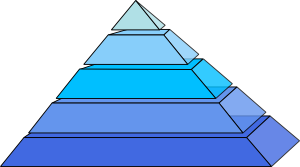
\includegraphics[width=1.1cm]{../Strukturfiler/FIGS/BluePyramid} & \begin{minipage}{\obsl}}{\end{minipage}\\ \end{tabular}\vspace{4mm}\newline}


% = Forudsætning = basis
\newenvironment{basis}{\begin{flushleft} \begin{itshape} }{\end{itshape} \end{flushleft}}


% = Opsummering =
\newenvironment{summary}{\clearpage\pagecolor{sumgul}\section{Opsummering}}{\newpage\pagecolor{white}}











% = Counter
\newcounter{opgavecount}[section]
\setcounter{opgavecount}{0}
\newcounter{spgcount}[opgavecount]
\setcounter{spgcount}{0}
\renewcommand{\thespgcount}{\alph{spgcount})}



% = EXERCISE = (DIVIDER)

\newcommand{\exercisebegin}[1][]{\bigskip\needspace{3\baselineskip}\refstepcounter{opgavecount}\titlegraphic{mingroen}\textcolor{mingroen}{\th{Opgave \theopgavecount \hspace*{1cm} #1}}\medskip\par}

% = QUIZEXERCISE = (DIVIDER)

\newcommand{\quizexercisebegin}[1][]{\bigskip\needspace{3\baselineskip}\refstepcounter{opgavecount}\titlegraphic{mingroen}\textcolor{mingroen}{\th{Quiz-Opgave \theopgavecount \hspace*{1cm} #1}}\medskip\par}

% = QUESTION =

\newenvironment{question}{\refstepcounter{spgcount}\begin{itemize}\item[\thespgcount]}{\end{itemize}\hspace*{\fill}}

% = VINK =

\newenvironment{vink}{\begin{tabular}{m{.9cm}<{\hspace*{2mm}}@{}|m{\obsl}@{}}\hspace*{-4pt}\raggedleft
\includegraphics[width=.9cm]{../Strukturfiler/FIGS/Think} & \begin{minipage}{\obsl}}{\end{minipage}\\ \end{tabular}\medskip\\}
	
% = FACIT =

\newenvironment{facit}{\begin{tabular}{m{.9cm}<{\hspace*{2mm}}@{}|m{\obsl}@{}}\hspace*{-4pt}\raggedleft
\includegraphics[width=.9cm]{../Strukturfiler/FIGS/Check} & \begin{minipage}{\obsl}}{\end{minipage}\\ \end{tabular}\medskip\\}








\newcommand{\afsnit}[1]{\bigskip\th{\titlegraphic{mingroen}\textcolor{mingroen}{#1}} \\ \rule[7pt]{.4\textwidth}{1pt} \vspace*{-2.5mm}\par}

% (DIVIDER):
\newcommand{\ugedagdatotitel}[4]{\pagebreak[4]\section{Semesteruge #1 -- #2 Dag \hspace*{1mm} (#3)} \vspace*{-4mm} \rule[5pt]{\textwidth}{1pt}\vspace*{-2.5mm} \begin{center}\large{\th{#4}}\end{center} \fancyhead[C]{\th{Semesteruge #1}}}

\newenvironment{skema}[1]{\definecolor{shadecolor}{rgb}{0.96,.98, 1.0} \setlength{\FrameSep}{6pt} \renewcommand{\FrameHeightAdjust}{10pt} \vspace*{-4pt}\begin{shaded} \begin{tabular}{#1}}{\end{tabular} \end{shaded} \vspace*{-7pt}}


% ========================

% MAKROER

%\newenvironment{matr}[1][]{\hspace*{-.8mm}\left[\hspace*{-1mm}\begin{array}{#1}}{\end{array}\hspace*{-1mm}\right]\hspace*{-.8mm}}
\newcommand{\bevisslut}{\begin{scriptsize} \begin{flushright} $ \blacksquare $ \end{flushright} \end{scriptsize}}

\newcommand{\tref}[2]{\hyperref[#1]{#2 \ref*{#1}}}
\newcommand{\thref}[2]{\hyperref[#1]{#2}}

\newcommand{\refA}[1]{\colorbox{yellow}{\ref{#1}}}
\newcommand{\hrefA}[2]{\colorbox{yellow}{\href{#1}{#2}}}
\newcommand{\trefA}[2]{\colorbox{yellow}{\hyperref[#1]{#2 \ref*{#1}}}}
\newcommand{\threfA}[2]{\colorbox{yellow}{\hyperref[#1]{#2}}}

\newenvironment{matr}[1]{\hspace*{-.8mm}\begin{bmatrix}\hspace*{-1mm}\begin{array}{#1}}{\end{array}\hspace*{-1mm}\end{bmatrix}\hspace*{-.8mm}}
\newcommand{\transp}{\hspace*{-.6mm}^{\top}}

\newcommand{\maengde}[2]{\left\lbrace \hspace*{-1mm} \begin{array}{c|c} #1 & #2 \end{array} \hspace*{-1mm} \right\rbrace}

\newenvironment{eqnalign}[1]{\setlength{\arraycolsep}{1.3pt}\begin{equation}\begin{array}{#1}}{\end{array}\end{equation}\par}
\newcommand{\eqnl}{\setlength{\arraycolsep}{1.3pt}}

\newcommand{\matind}[3]{{_\mathrm{#1}\mathbf{#2}_\mathrm{#3}}}
\newcommand{\vekind}[2]{{_\mathrm{#1}\mathbf{#2}}}
\newcommand{\jac}[2]{{\mathrm{Jacobi}_\mathbf{#1} (#2)}}
\newcommand{\diver}[2]{{\mathrm{div}\mathbf{#1} (#2)}}
\newcommand{\rot}[1]{{\mathbf{rot}\mathbf{(#1)}}}

\newcommand{\am}{\mathrm{am}}
\newcommand{\gm}{\mathrm{gm}}
\newcommand{\E}{\mathrm{E}}
\newcommand{\Span}{\mathrm{span}}
\newcommand{\mU}{\mathbf{U}}

\newcommand{\ms}{\medskip\\}
\newcommand{\bs}{\bigskip\\}

\newcommand{\mA}{\mathbf{A}}
\newcommand{\mB}{\mathbf{B}}
\newcommand{\mC}{\mathbf{C}}
\newcommand{\mD}{\mathbf{D}}
\newcommand{\mE}{\mathbf{E}}
\newcommand{\mF}{\mathbf{F}}
\newcommand{\mK}{\mathbf{K}}
\newcommand{\mI}{\mathbf{I}}
\newcommand{\mM}{\mathbf{M}}
\newcommand{\mN}{\mathbf{N}}
\newcommand{\mQ}{\mathbf{Q}}
\newcommand{\mT}{\mathbf{T}}
\newcommand{\mV}{\mathbf{V}}
\newcommand{\mW}{\mathbf{W}}
\newcommand{\mX}{\mathbf{X}}
\newcommand{\ma}{\mathbf{a}}
\newcommand{\mb}{\mathbf{b}}
\newcommand{\mc}{\mathbf{c}}
\newcommand{\md}{\mathbf{d}}
\newcommand{\me}{\mathbf{e}}
\newcommand{\mn}{\mathbf{n}}
\newcommand{\mr}{\mathbf{r}}
\newcommand{\mv}{\mathbf{v}}
\newcommand{\mw}{\mathbf{w}}
\newcommand{\mx}{\mathbf{x}}
\newcommand{\mxb}{\mathbf{x_{bet}}}
\newcommand{\my}{\mathbf{y}}
\newcommand{\mz}{\mathbf{z}}
\newcommand{\reel}{\mathbb{R}}
\newcommand{\mL}{\bm{\Lambda}} %Lambda-matrix
\newcommand{\mnul}{\bm{0}}
\newcommand{\trap}[1]{\mathrm{trap}(#1)}
\newcommand{\Det}{\operatorname{Det}}
\newcommand{\adj}{\operatorname{adj}}
\newcommand{\Ar}{\operatorname{Areal}}
\newcommand{\Vol}{\operatorname{Vol}}
\newcommand{\Rum}{\operatorname{Rum}}
\newcommand{\diag}{\operatorname{\bf{diag}}}
\newcommand{\bidiag}{\operatorname{\bf{bidiag}}}
\newcommand{\spanVec}[1]{\mathrm{span}\{#1\}}
\newcommand{\Div}{\operatorname{Div}}
\newcommand{\Rot}{\operatorname{\mathbf{Rot}}}

\newcommand{\Jac}{\operatorname{Jacobi}}
\newcommand{\Tan}{\operatorname{Tan}}
\newcommand{\Ort}{\operatorname{Ort}}
\newcommand{\Flux}{\operatorname{Flux}}
\newcommand{\Cmass}{\operatorname{Cm}}
\newcommand{\Imom}{\operatorname{Im}}
\newcommand{\Pmom}{\operatorname{Pm}}
\newcommand{\IS}{\operatorname{I}}
\newcommand{\IIS}{\operatorname{II}}
\newcommand{\IIIS}{\operatorname{III}}
\newcommand{\Le}{\operatorname{L}}
\newcommand{\app}{\operatorname{app}}
\newcommand{\M}{\operatorname{M}}
\newcommand{\re}{\mathrm{Re}}
\newcommand{\im}{\mathrm{Im}}

\newcommand{\compl}{\mathbb{C}} %de komplekse tal
\newcommand{\e}{\mathrm{e}} %eksponentialfunktionen. lodret 'e', og altså ikke kursiv ligesom andre bogstaver.





% Medialink: SCREEN: (QRcode) + thumbnail image + link på kodenummer (til qr.dtu.dk)
\newcommand{\onlinemedia}[3]{
	\begin{wrapfigure}{r}{3.2cm} 
		\vspace{-30pt} 
		\vspace{#1pt} 
		\begin{flushright} 
			\includegraphics[width=3cm]{qr/#2.png} 
			\tiny 
			\href{http://qr.dtu.dk/#2}{#2: #3}
			\normalsize  
		\end{flushright} 
		\vspace{-10pt} 
	\end{wrapfigure}
}
\newcommand{\onlinemediathumb}[3]{
	\begin{wrapfigure}{r}{3.2cm} 
		\vspace{-30pt} 
		\vspace{#1pt} 
		\begin{flushright} 
			\includegraphics[width=3cm]{qr/#2.png} 
			\includegraphics[width=3cm]{qr/#2_thumb.png} 
			\tiny 
			\href{http://qr.dtu.dk/#2}{#2: #3}
			\normalsize  
		\end{flushright} 
		\vspace{-10pt} 
	\end{wrapfigure}
}



% Index:
\usepackage{makeidx}
\makeindex
\newcommand\ind[2]{\index{#1}\textbf{\textit{\textcolor{black}{#2}}}}

% ###SERVER_EXCLUDE_BEGIN###
\externaldocument[NUID17-]{../../enoten/TN01-Talrum/Talrum}
\externaldocument[NUID1-]{../../enoten/TN02-Ligningssystemer/TNdriver}
\externaldocument[NUID2-]{../../enoten/TN03-Matricer_og_Matrixalgebra/Matricer_og_matrixalgebra}
\externaldocument[NUID3-]{../../enoten/TN04-Kvadratiske_matricer/TNdriver}
\externaldocument[NUID11-]{../../enoten/TN05-Determinanter/Determinanter}
\externaldocument[NUID12-]{../../enoten/TN06-GeometriskeVektorer/GeometriskeVektorer}
\externaldocument[NUID18-]{../../enoten/TN07-Vektorrum/VektorRum}
\externaldocument[NUID21-]{../../enoten/TN08-LinAfbildninger/LinAfbildninger}
\externaldocument[NUID23-]{../../enoten/TN09-Egenvaerdier_og_egenvektorer/TNdriver}
\externaldocument[NUID24-]{../../enoten/TN10-Diagonalisering_med_egenvektorer/TNdriver}
\externaldocument[NUID10-]{../../enoten/TN11-1.ordens_differentialligninger/TNdriver}
\externaldocument[NUID13-]{../../enoten/TN12-1.ordens_differentialligningssystemer/TNdriver}
\externaldocument[NUID14-]{../../enoten/TN13-2.ordens_differentialligninger/TNdriver}
\externaldocument[NUID27-]{../../enoten/TN14-Elemenataere_funktioner/Elementaere_Funktioner}
\externaldocument[NUID28-]{../../enoten/TN15-Funktioner2Variable/Funktioner_To_Variable}
\externaldocument[NUID29-]{../../enoten/TN16-Gradienter_og_Tangentplaner/Gradienter_og_Tangentplaner}
\externaldocument[NUID32-]{../../enoten/TN17-Taylor_formler/Taylor_Formler}
\externaldocument[NUID33-]{../../enoten/TN18-Taylor_2Var/Taylor_2Var}
\externaldocument[NUID34-]{../../enoten/TN19-SymMat/SymmetriskeMatricer}
\externaldocument[NUID35-]{../../enoten/TN20-KegleSnit/Keglesnit}
\externaldocument[NUID36-]{../../enoten/TN21-Riemann_Integral/Riemann_01}
\externaldocument[NUID37-]{../../enoten/TN22-Plan_Int/Plan_Int_01}
\externaldocument[NUID39-]{../../enoten/TN23-Flade_Int/Flade_Rum_Int_01}
\externaldocument[NUID40-]{../../enoten/TN24-Vektorfelter/Vektorfelter_01}
\externaldocument[NUID41-]{../../enoten/TN25-Flux/Flux_02}
\externaldocument[NUID42-]{../../enoten/TN26-Gauss/Gauss_01}
\externaldocument[NUID128-]{../../enoten/TN27-Stokes/Stokes_01}
\externaldocument[NUID43-]{../../enoten/TN29-KomplekseTal/KomplekseTal}

\externaldocument[NUID6-]{../../E-math-opgaver/Opgaver/opgU123}
\externaldocument[NUID19-]{../../E-math-opgaver/Opgaver/opgU45}
\externaldocument[NUID20-]{../../E-math-opgaver/Opgaver/opgU678}
\externaldocument[NUID25-]{../../E-math-opgaver/Opgaver/opgU910SD}
\externaldocument[NUID31-]{../../E-math-opgaver/OpgaverF11-U123/opgF123}
% \externaldocument[NUID9-]{../../E-math-opgaver/Opgaver/Dagsordner E10}
% ###SERVER_EXCLUDE_END###


% Begin document and set alternative chapter title:
\begin{document}
\renewcommand{\chaptername}{eNote}

\setcounter{chapter}{19} %SÆT DETTE TAL TIL 1 MINDRE END DET AKTUELLE TRANSFERNOTE-NUMMER!!

%%%%%%%%%%%%%%%%%%%%%%%%%%%%%%%%%%%%%%%%%%%%%
%%%%%%%%%%%%%%%%%%%%%%%%%%%%%%%%%%%%%%%%%%%%%
%%% HERFRA SKAL DU SKRIVE ELLER INDSÆTTE %%%%
%%% DEN FIL DU ØNSKER %%%%%%%%%%%%%%%%%%%%%%%
%%%%%%%%%%%%%%%%%%%%%%%%%%%%%%%%%%%%%%%%%%%%%
%%%%%%%%%%%%%%%%%%%%%%%%%%%%%%%%%%%%%%%%%%%%%

\chapter{Andengradsligninger i to og tre  variable} \label{tn20}




\begin{basis}
I denne eNote vil vi igen beskæftige os med andengradspolynomierne i to og tre variable
som også er behandlet og undersøgt med forskellige teknikker i henholdsvis \tref{NUID33-tn18}{eNote} og  \tref{NUID34-tn19}{eNote}.
Ved den indledende behandling af funktioner af to variable definerede vi niveau-mængderne $\mathcal{K}_{c}(f)$ for funktioner $f(x,y)$ af to variable, se \tref{NUID28-tn15}{eNote}.
Vi skal se i denne eNote, at for andengradspolynomier i to variable er niveaumængderne typisk velkendte kurver i $(x,y)$-planen som for  eksempel
ellipser og hyperbler og det er formålet med denne eNote at vise hvilke typer niveaukurver der optræder for givne ligninger. Vi vil dertil i udstrakt grad benytte den reduktionsmetode, der er udviklet i \tref{NUID33-tn18}{eNote}. Den virker for andengradspolynomier af både to og tre (og flere) variable, og som vi skal se, kan de tilhørende niveau-kurver og -flader identificeres ud fra en kort navneliste. Niveaukurverne for andengradspolymier i to variable og niveaufladerne for andengradspolynomier i tre variable  kendes klassisk under navnene henholdsvis \ind{keglesnit}{keglesnit} og \ind{keglesnitsflader}{keglesnitsflader}.
\end{basis}



%%%%%%%%%%%%%%%%%%%%%%%%%%%%%%%%%%%%%%%%%%%%%%%%%%%%%%%%%%%%%
%%%%%%%%%%%%%%%%%%%%%%%%%%%%%%%%%%%%%%%%%%%%%%%%%%%%%%%%%%%%%
%%%%%%%%%%%%%%%%%%%%%%%%%%%%%%%%%%%%%%%%%%%%%%%%%%%%%%%%%%%%%


\section{Andengradsligninger i to variable}

Fra \tref{NUID33-tn18}{eNote} ved vi fra inspektion af de viste niveaukurver, at der typisk optræder ellipser og hyperbler
eller ellipse-lignende og hyperbel-lignende kurver som niveaukur\-ver for funktioner af to variable -- især omkring stationære punkter. Det er ikke nogen tilfældighed; andengradspolynomier har netop sådanne niveaukurver.  Og passende valg\-te andengradspolynomier er jo samtidig gode approksimationer til givne glatte funktioner af to variable.\\


I det følgende vil vi med nogle eksempler gennemgå standardmetoden til reduktion af de ligninger, der fremkommer når vi vil finde de punkter i $\mathbb{R}^{2}$ for hvilke et givet andengradspolynomium er $0$, altså netop de punkter, der udgør niveaumængden $\mathcal{K}_{0}(f)$ for $f(x,y)$.


\begin{example}[Ellipse] \label{exampEllip01}
For et andengradspolynomium $f(x,y)$ bestemmer vi følgende ingredienser til reduktion af polynomiet på præcis den måde som er gennemgået i \tref{NUID33-tn18}{eNote}. Vi har specielt igen brug for den positive ortogonale substitutionsmatrix $\mathbf{Q}$ som diagonaliserer matricen $\frac{1}{2}\cdot \mathbf{H}f(x,y)$ for derved at opnå et udtryk for $f(x,y)$ som ikke indeholder produkt\-led -- nu i de nye koordianter $\widetilde{x}$ og $\widetilde{y}$. Resultatet af reduktionen er $\widetilde{f}(\widetilde{x}, \widetilde{y})$ som vist nedenfor:
\begin{equation}
\begin{aligned}
f(x,y) &= 2\cdot x^{2} + 2\cdot y^{2} + 2\cdot x\cdot y -8\cdot x -10 \cdot y + 13 \quad . \\  \\
\bm{\nabla}f(x,y) &= (4\cdot x +2\cdot y-8\, , \,2\cdot x + 4\cdot y -10) \quad . \\  \\
\frac{1}{2}\cdot \mathbf{H}f(x,y) &= \left[
                     \begin{array}{cc}
                       2 & 1 \\
                       1 & 2 \\
                     \end{array}
                   \right] \quad . \\ \\
\bm{\Lambda} &= \left[
                     \begin{array}{cc}
                       3 & 0 \\
                       0 & 1 \\
                     \end{array}
                   \right] \quad . \\ \\
\mathbf{Q} &= \left[
                     \begin{array}{cc}
                       \sqrt{2}/2 & -\sqrt{2}/2 \\
                       \sqrt{2}/2 & \sqrt{2}/2 \\
                     \end{array}
                   \right] = \left[
                     \begin{array}{cc}
                       \cos(\pi/4) & -\sin(\pi/4) \\
                        \sin(\pi/4) &  \cos(\pi/4)\\
                     \end{array}
                   \right] \quad . \\ \\
\widetilde{f}(\widetilde{x}, \widetilde{y}) & = 3\cdot \widetilde{x}^{2} + \widetilde{y}^{2} - 9\cdot\sqrt{2}\cdot\widetilde{x} - \sqrt{2}\cdot\widetilde{y} +13 \\
&= 3\cdot\left(\widetilde{x} - \frac{3}{2}\cdot\sqrt{2} \right)^{2} + \left(\widetilde{y} - \frac{1}{2}\cdot\sqrt{2} \right)^{2} -1 \quad. \\
\end{aligned}
\end{equation}
Den sidste ligning i ovenstående beregning af det reducerede andengradspolynomium $\widetilde{f}(\widetilde{x}, \widetilde{y})$ fremkommer ved \ind{kvadratkomplettering}{kvadratkomplettering}. Den kan foretages for  $\widetilde{x}$-leddene først og dernæst for $\widetilde{y}$-leddene. For de førstnævnte foregår det sådan:

\begin{equation}
\begin{aligned}
3\cdot \widetilde{x}^{2} - 9\cdot\sqrt{2}\cdot \widetilde{x} &= 3\cdot (\widetilde{x}^{2} - 3\cdot \sqrt{2} \cdot \widetilde{x}) \\
&= 3\cdot \left( \left(\widetilde{x} - \frac{3}{2}\sqrt{2}\right)^{2} - \frac{9}{2}\right) \quad.
\end{aligned}
\end{equation}


Den andengradsligning som giver niveaukurven $\mathcal{K}_{0}(f)$ er nu  bestemt ved hver af følgende ækvivalente ligninger:
\begin{equation}
\begin{aligned}
f(x,y) &= 0 = \widetilde{f}(\widetilde{x}, \widetilde{y})  \\ \\
\left(\frac{\widetilde{x} - \frac{3}{2}\cdot\sqrt{2}}{\frac{1}{\sqrt{3}}}\right)^{2} &+ \left(\widetilde{y} - \frac{1}{2}\cdot\sqrt{2} \right)^{2} = 1 \quad .
\end{aligned}
\end{equation}
Denne sidste ligning fremstiller en {\emph{ellipse}} med centrum i $\vekind{e}{\mathbf{C}} = (x_{0}, y_{0}) =  (1,2)$ (med hensyn til de gamle koordinater) svarende til
$\vekind{v}{\mathbf{C}} = (\widetilde{x}_{0}, \widetilde{y}_{0}) =  (\frac{3}{2}\cdot\sqrt{2}\, , \, \frac{1}{2}\cdot\sqrt{2} )$ (med hensyn til de nye koordinater)  og halvakserne $\frac{1}{\sqrt{3}}$ og  $1$ , se figurerne \ref{figEllip01} og  \ref{figEllip01Kvad}. Det nye koordinatsystem fremkommer ved drejning af det gamle koordinatsystem med drejningsvinklen $\phi = \pi/4$. \\

Funktionen $f(x,y)$ har  et stationært punkt i centrum for ellipsen, hvor funktionsværdien er $-1$. Hesse-matricen er positiv definit og derfor er det stationære punkt et egentligt lokalt minimumpunkt. Der er tydeligvis tale om et globalt minimumpunkt.

\end{example}


\begin{figure}[ht]
\centerline{ 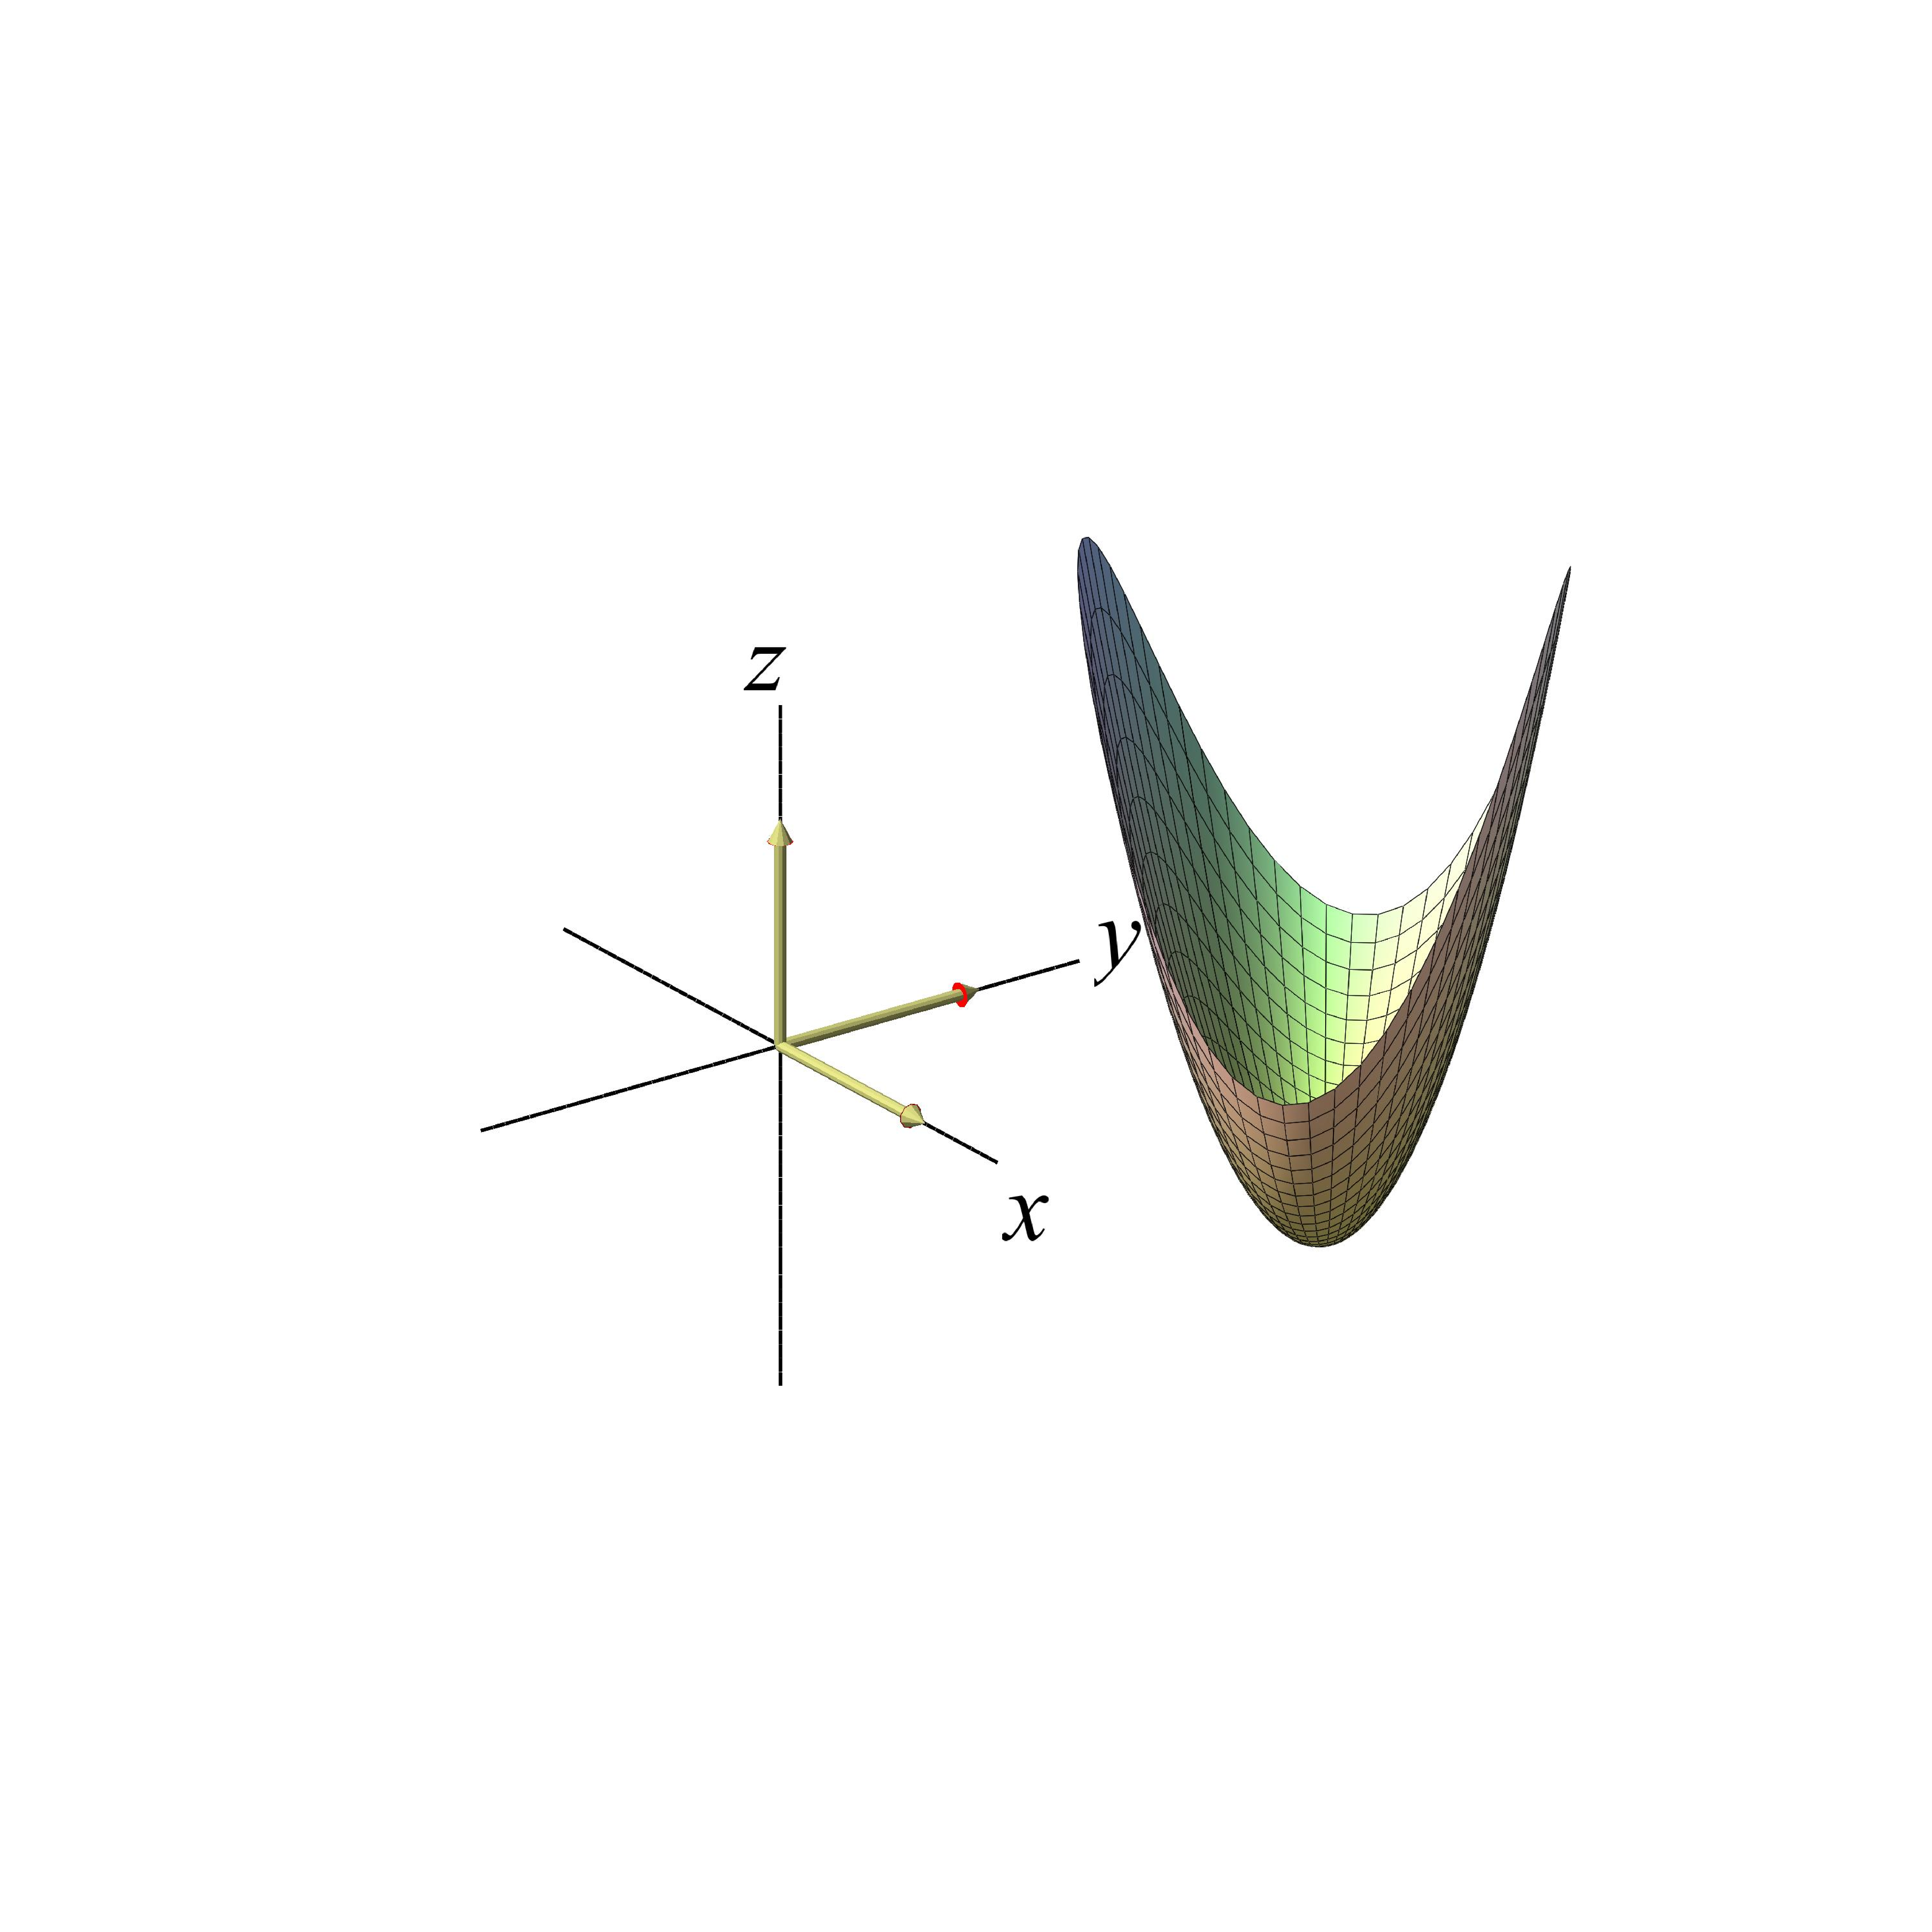
\includegraphics[height=60mm]{FIGS/plot2DEllipLift01.pdf} 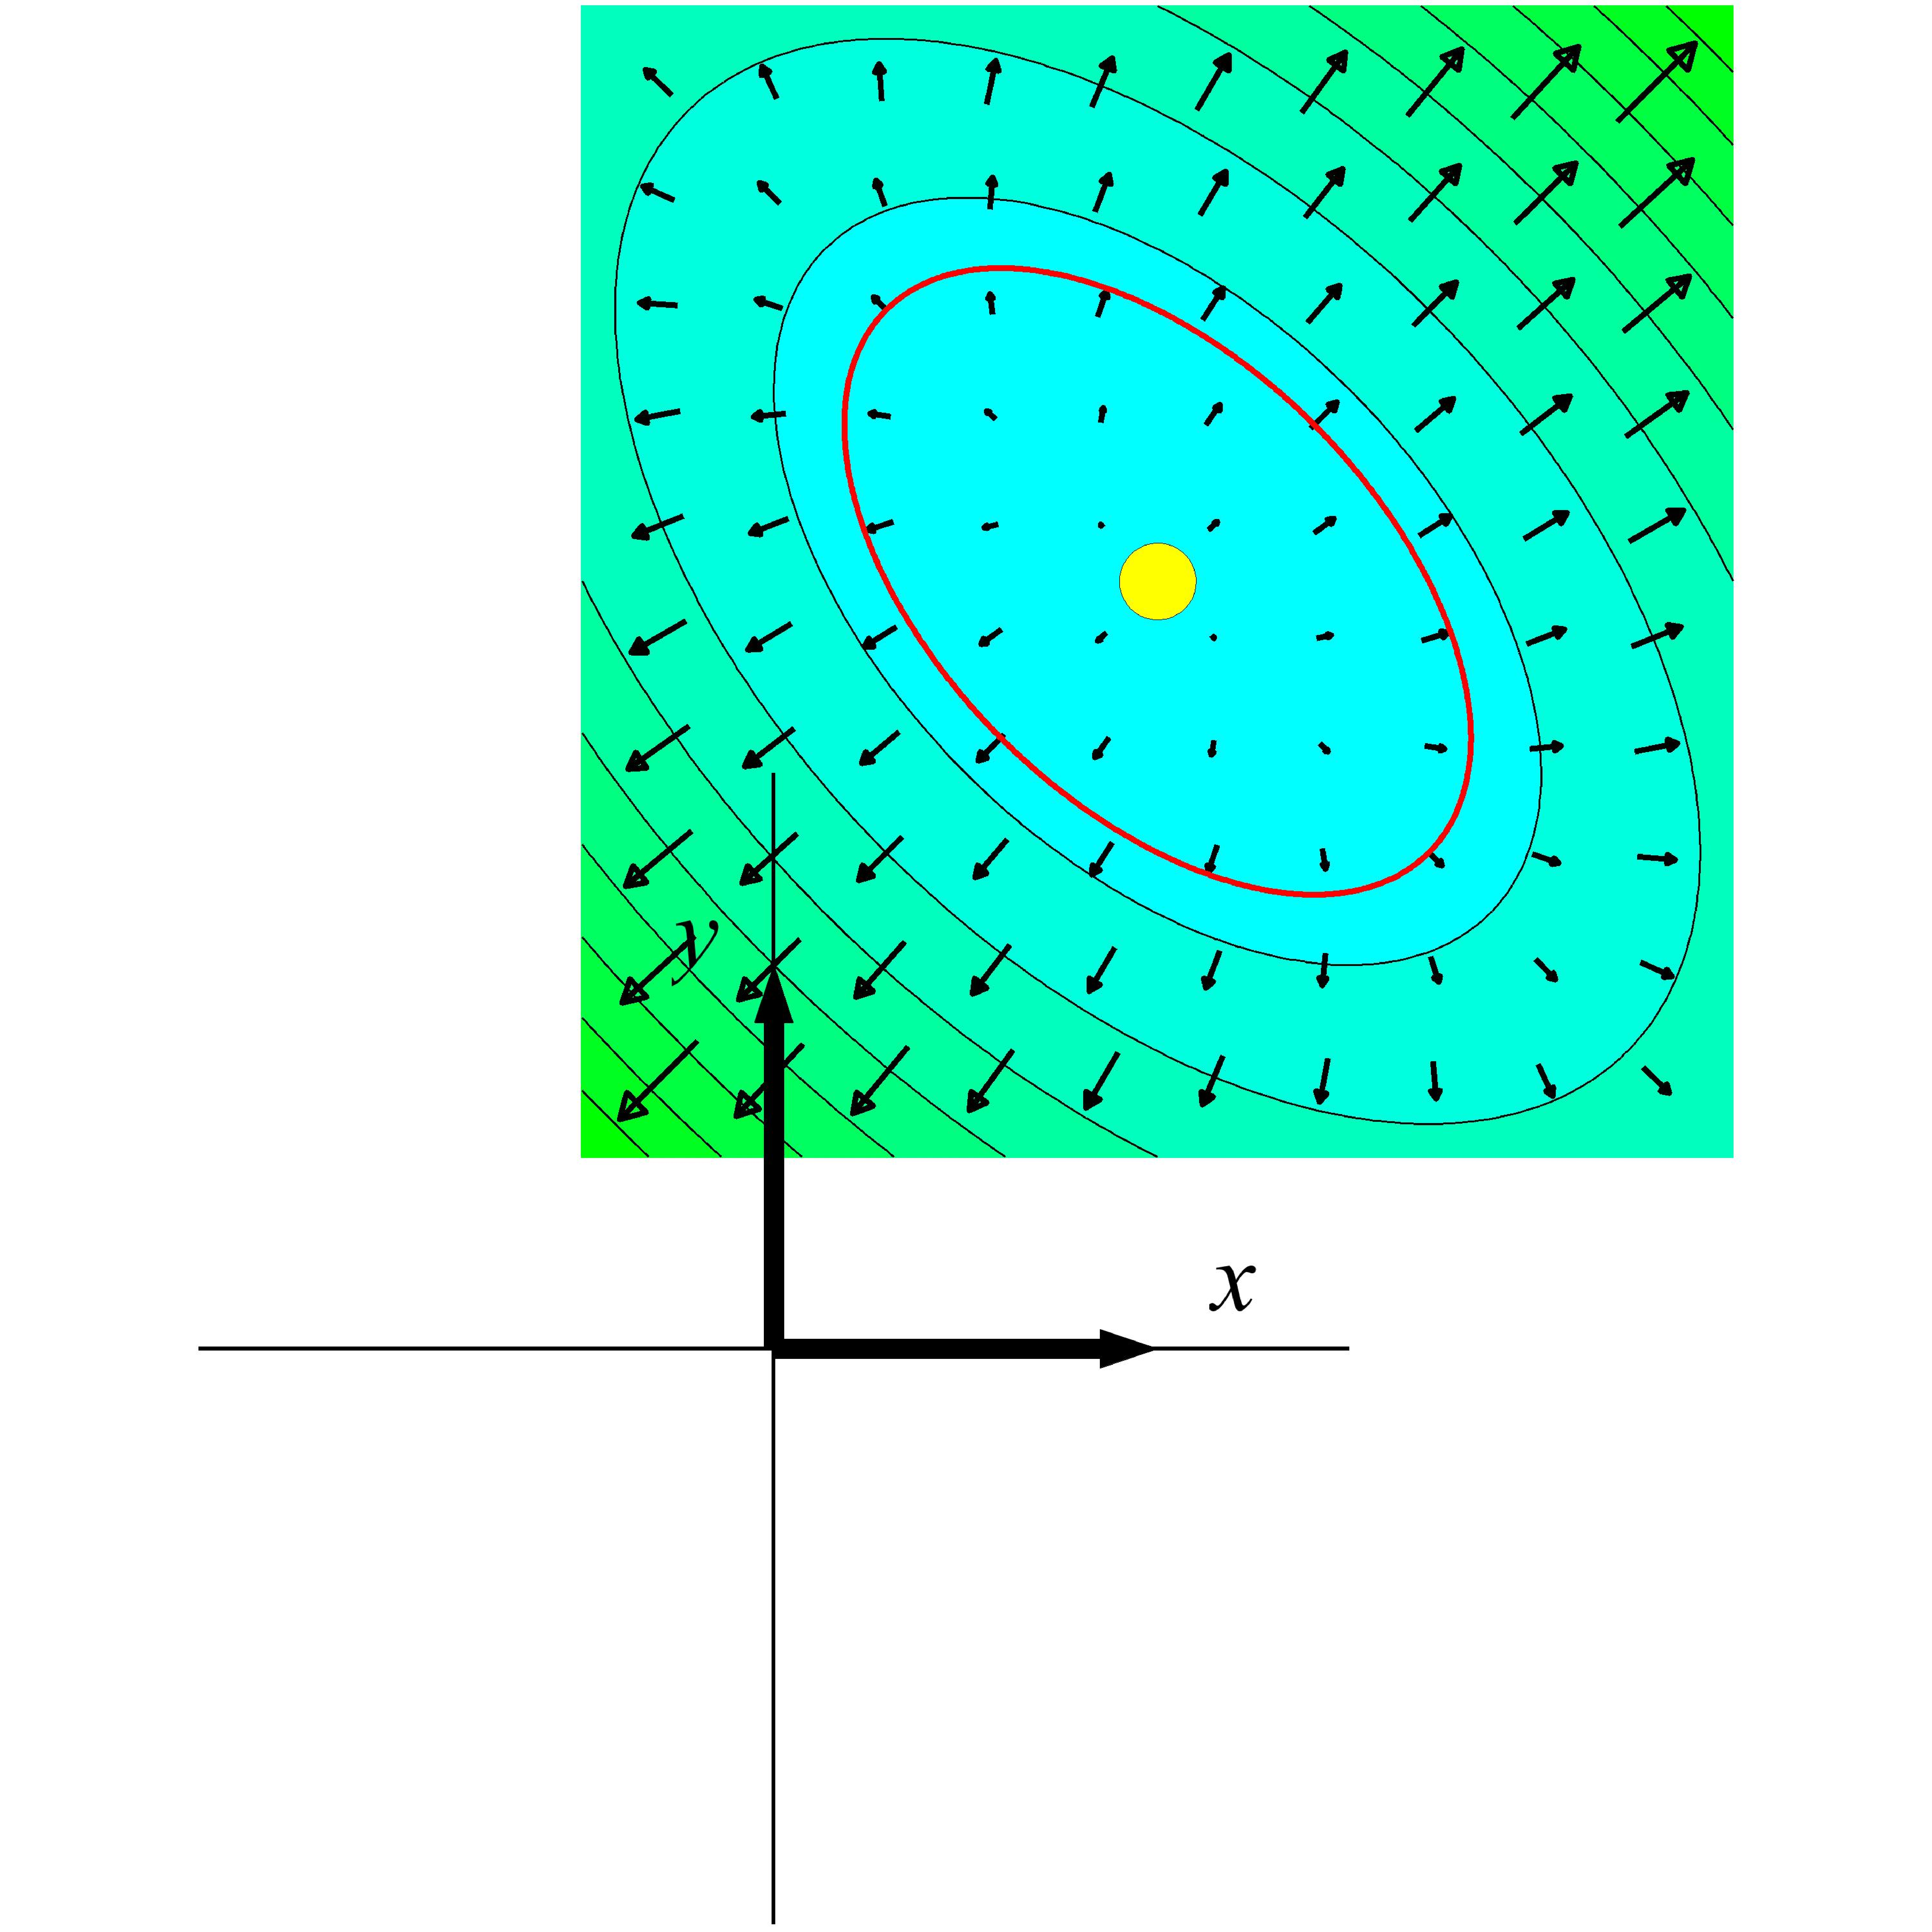
\includegraphics[height=60mm]{FIGS/plot2DGradEllip01.pdf}}
\begin{center}
\caption{Grafen for funktionen $f(x,y) = 2\cdot x^{2} + 2\cdot y^{2} + 2\cdot x\cdot y -8\cdot x -10 \cdot y + 13 $ samt niveaukurver og gradientvektorfelt for funktionen. Bemærk specielt niveaukurven svarende til niveau $0$, som er den ellipse vi analyserer i eksempel \ref{exampEllip01}.} \label{figEllip01}
\end{center}
\end{figure}


\begin{figure}[ht]
\centerline{  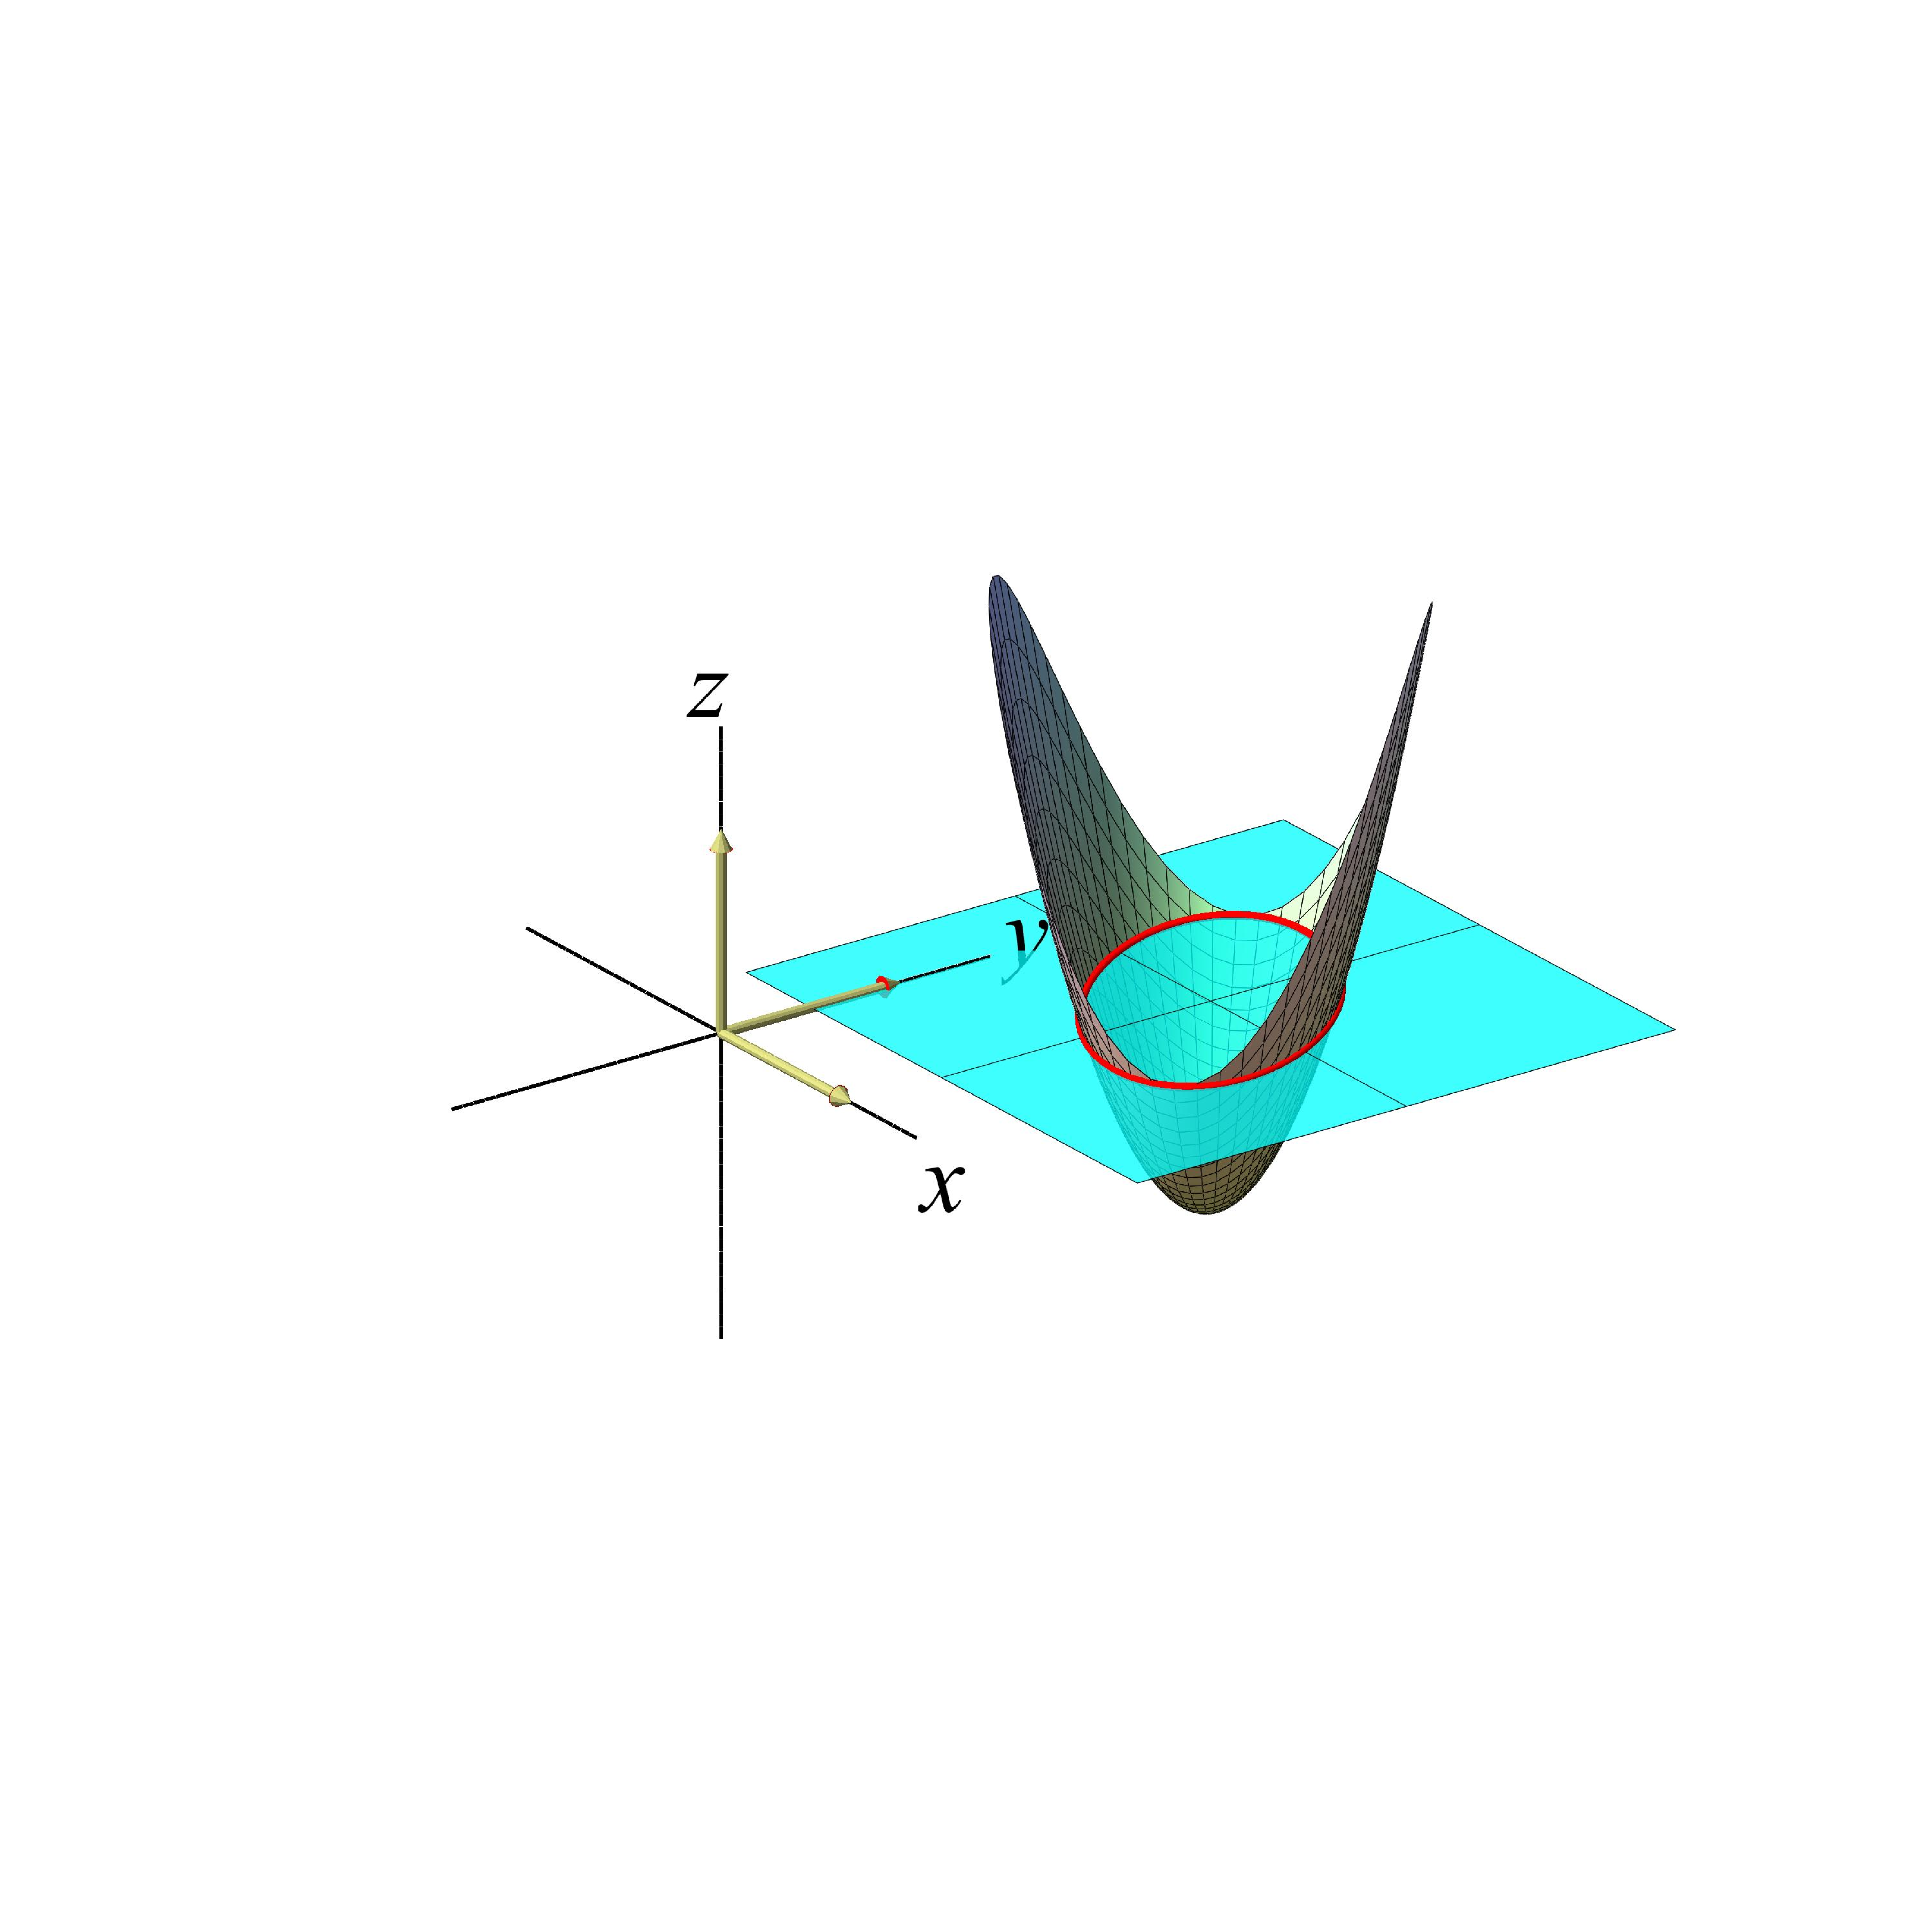
\includegraphics[height=60mm]{FIGS/plot2DNivEllipLift01.pdf} 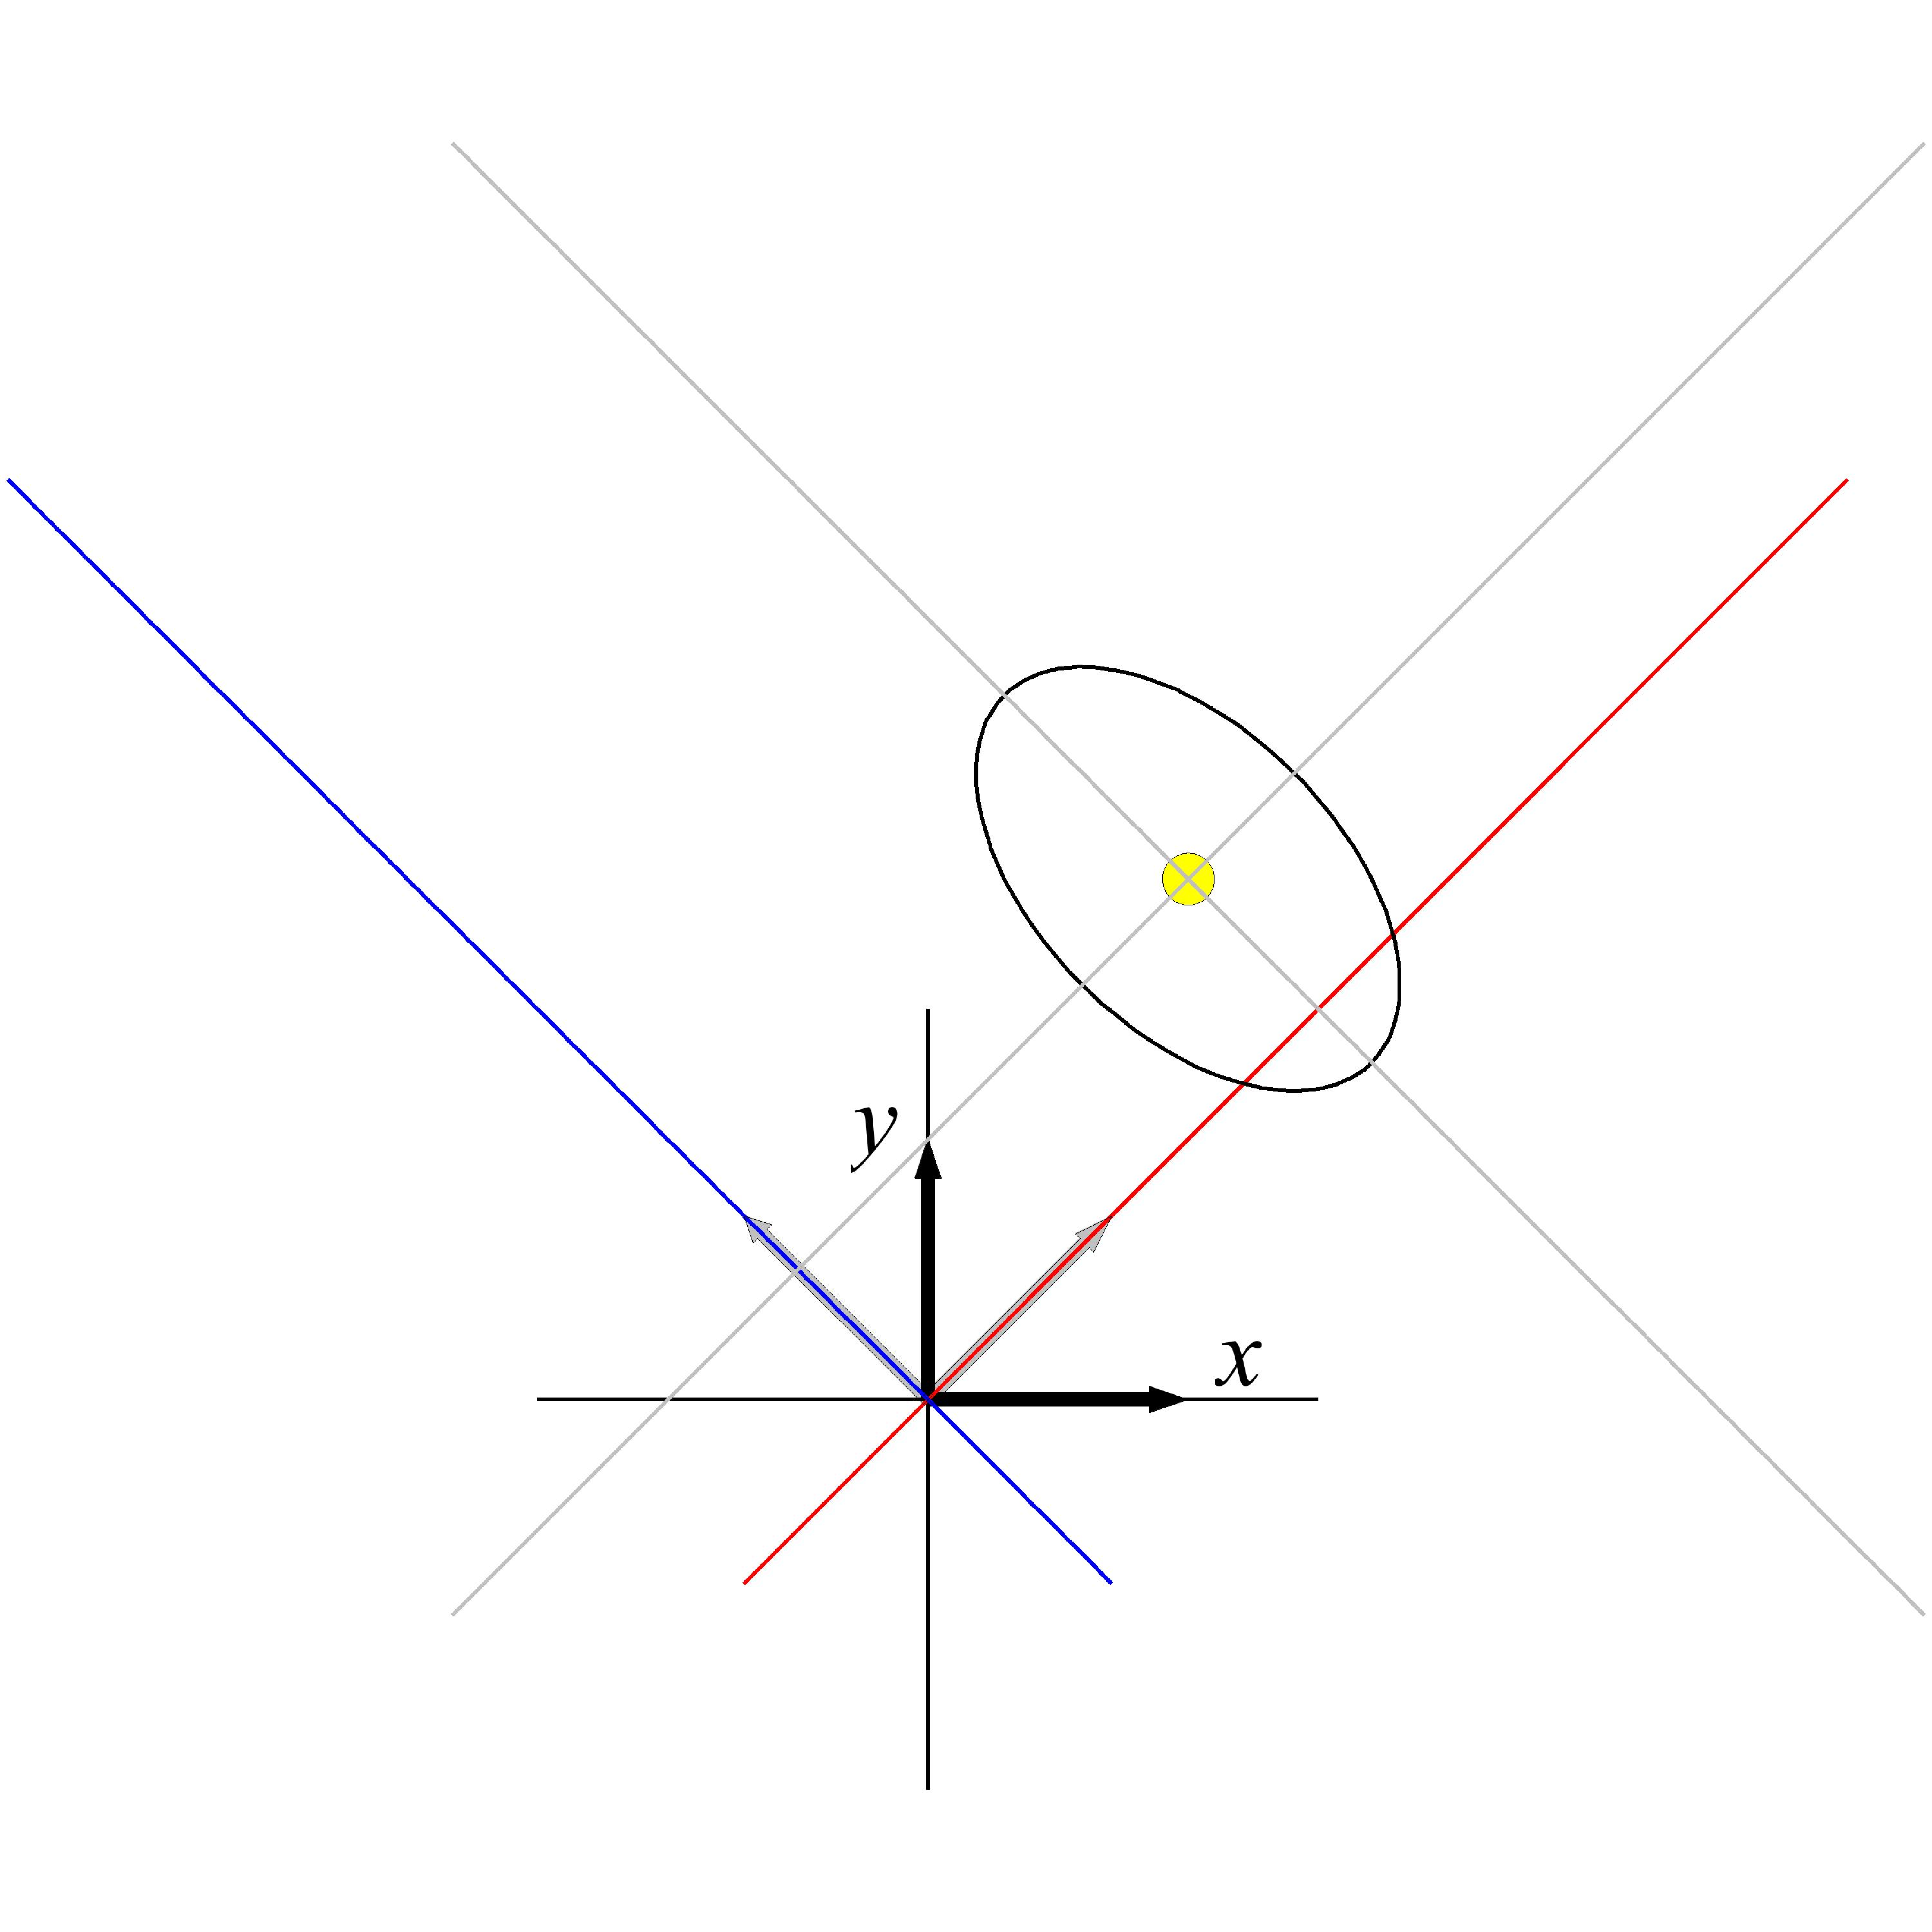
\includegraphics[height=60mm]{FIGS/plotEllipKvad01.pdf}}
\begin{center}
\caption{Grafen for funktionen med den elliptiske niveaukurve i niveau $0$ for funktionen i eksempel \ref{exampEllip01}.} \label{figEllip01Kvad}
\end{center}
\end{figure}


\begin{figure}[ht]
\centerline{  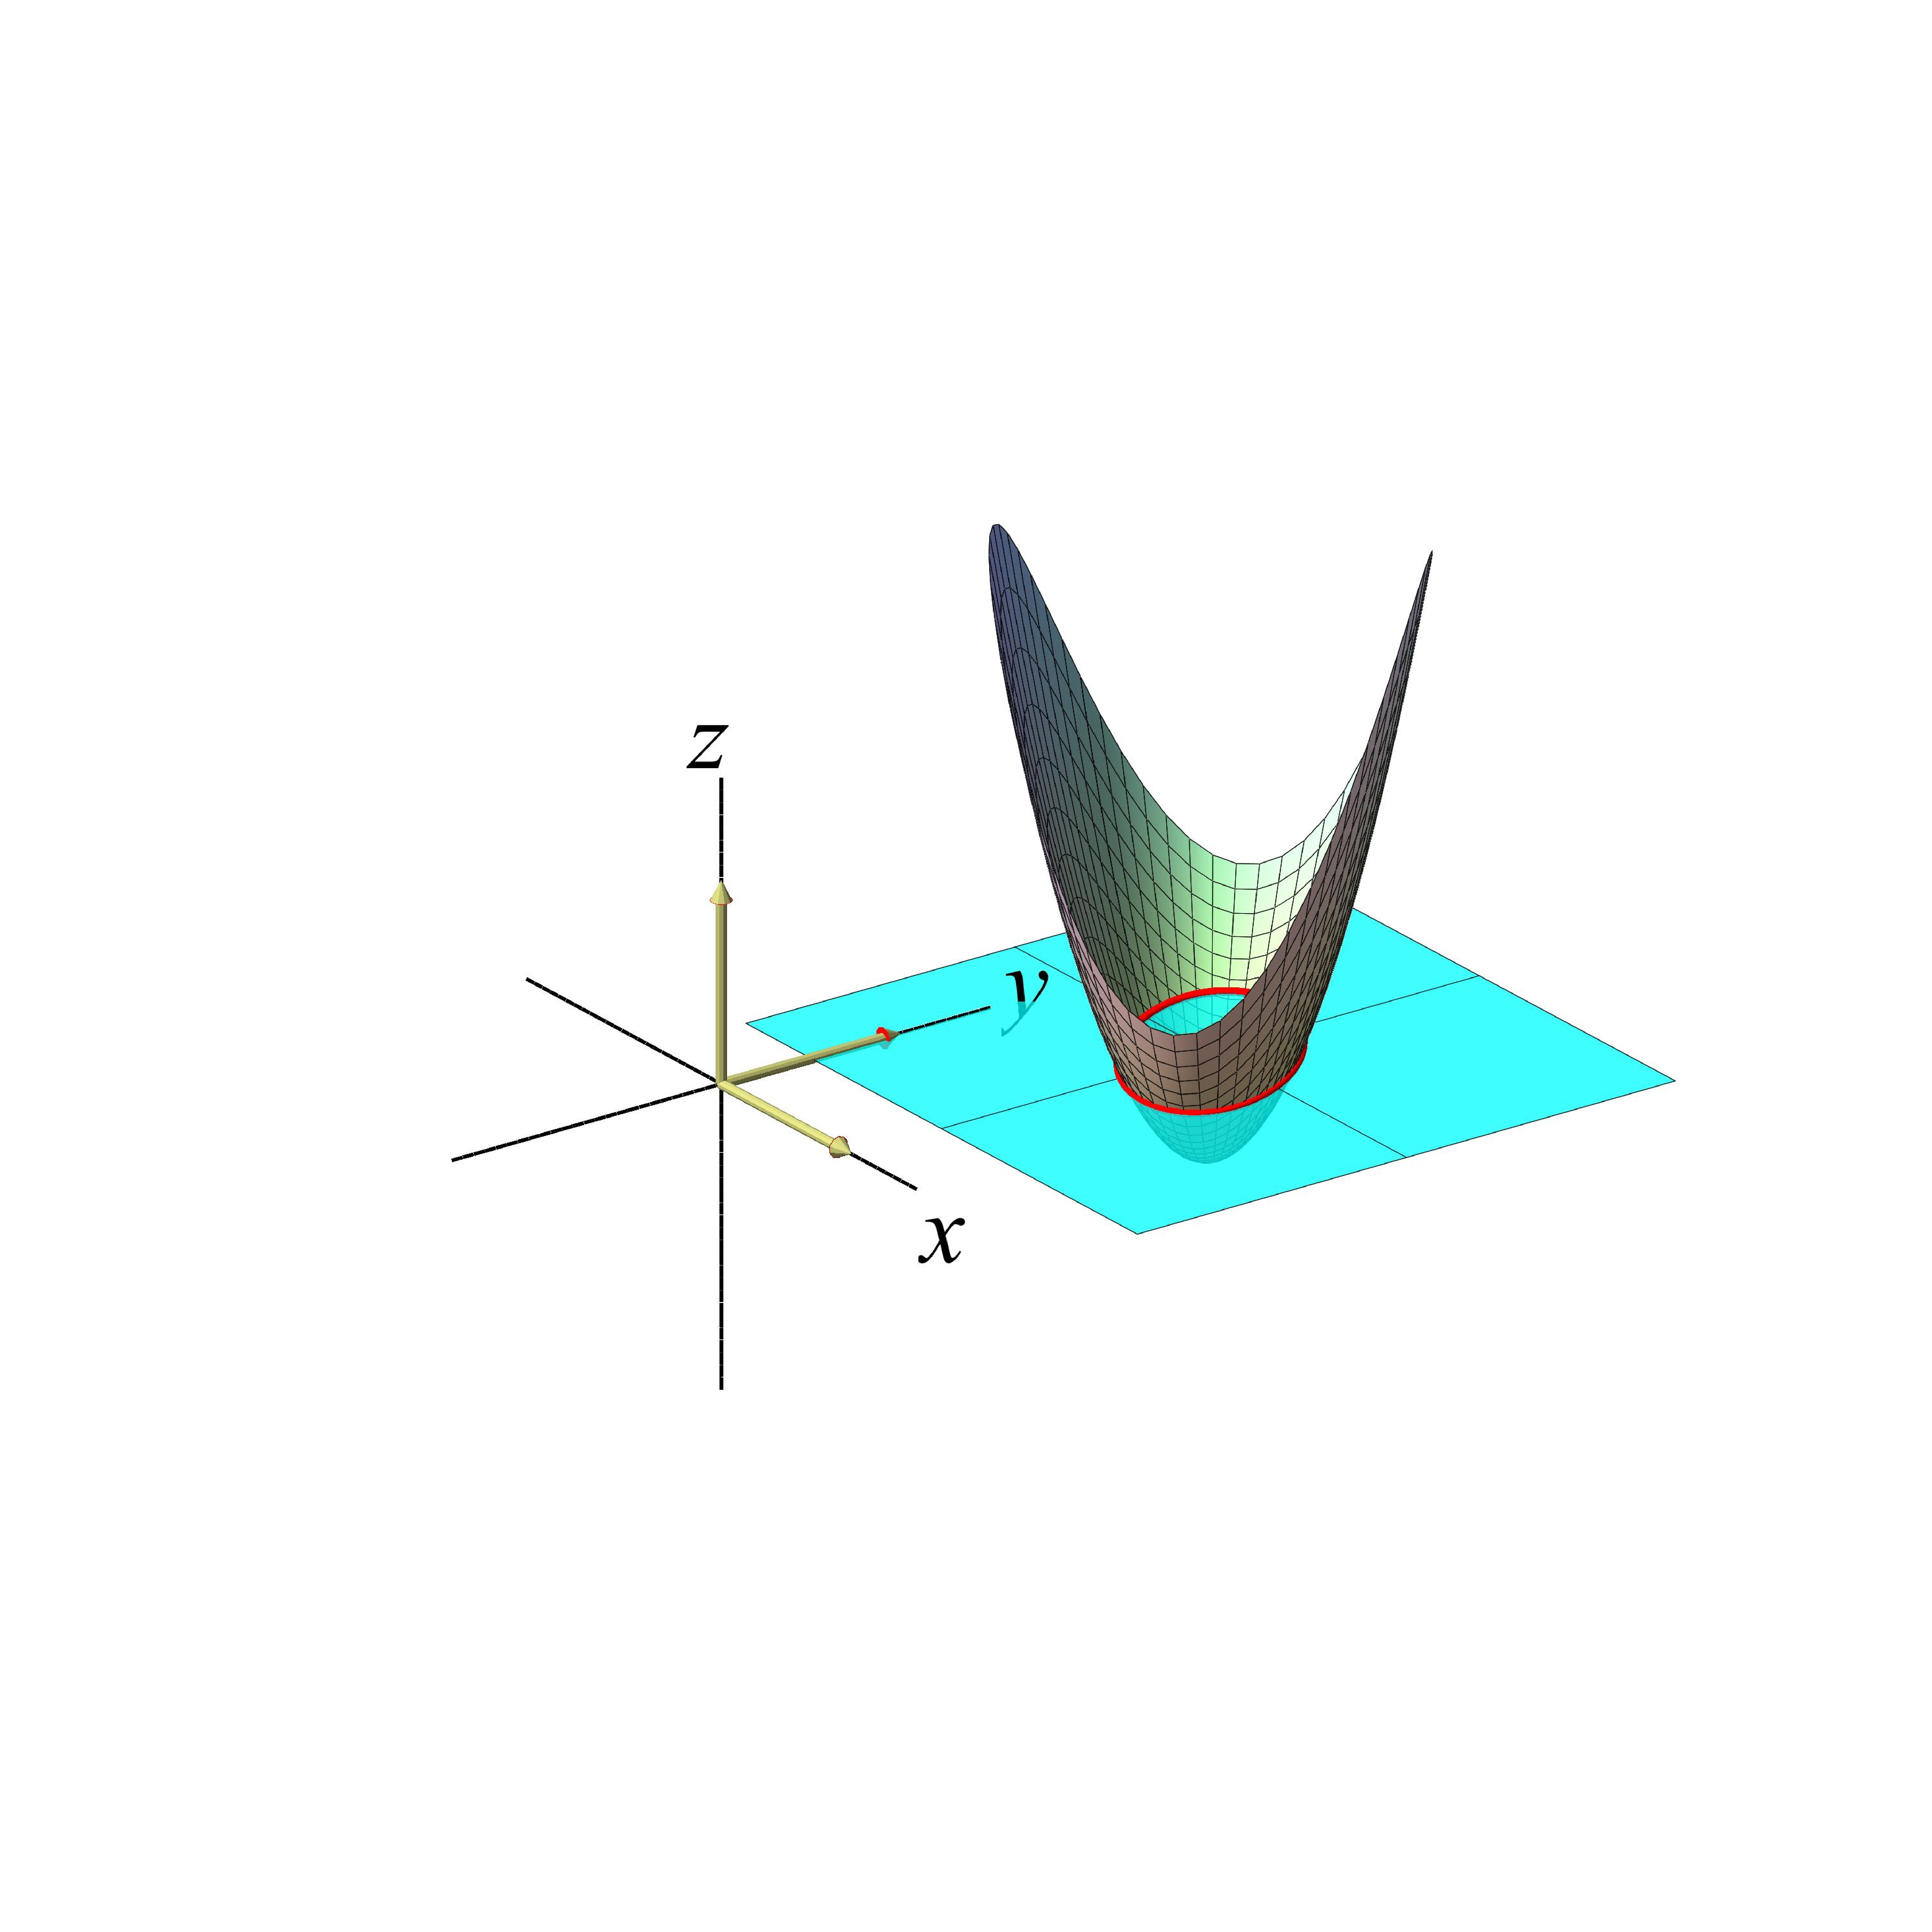
\includegraphics[height=60mm]{FIGS/plot2DNivEllipLift02.pdf} 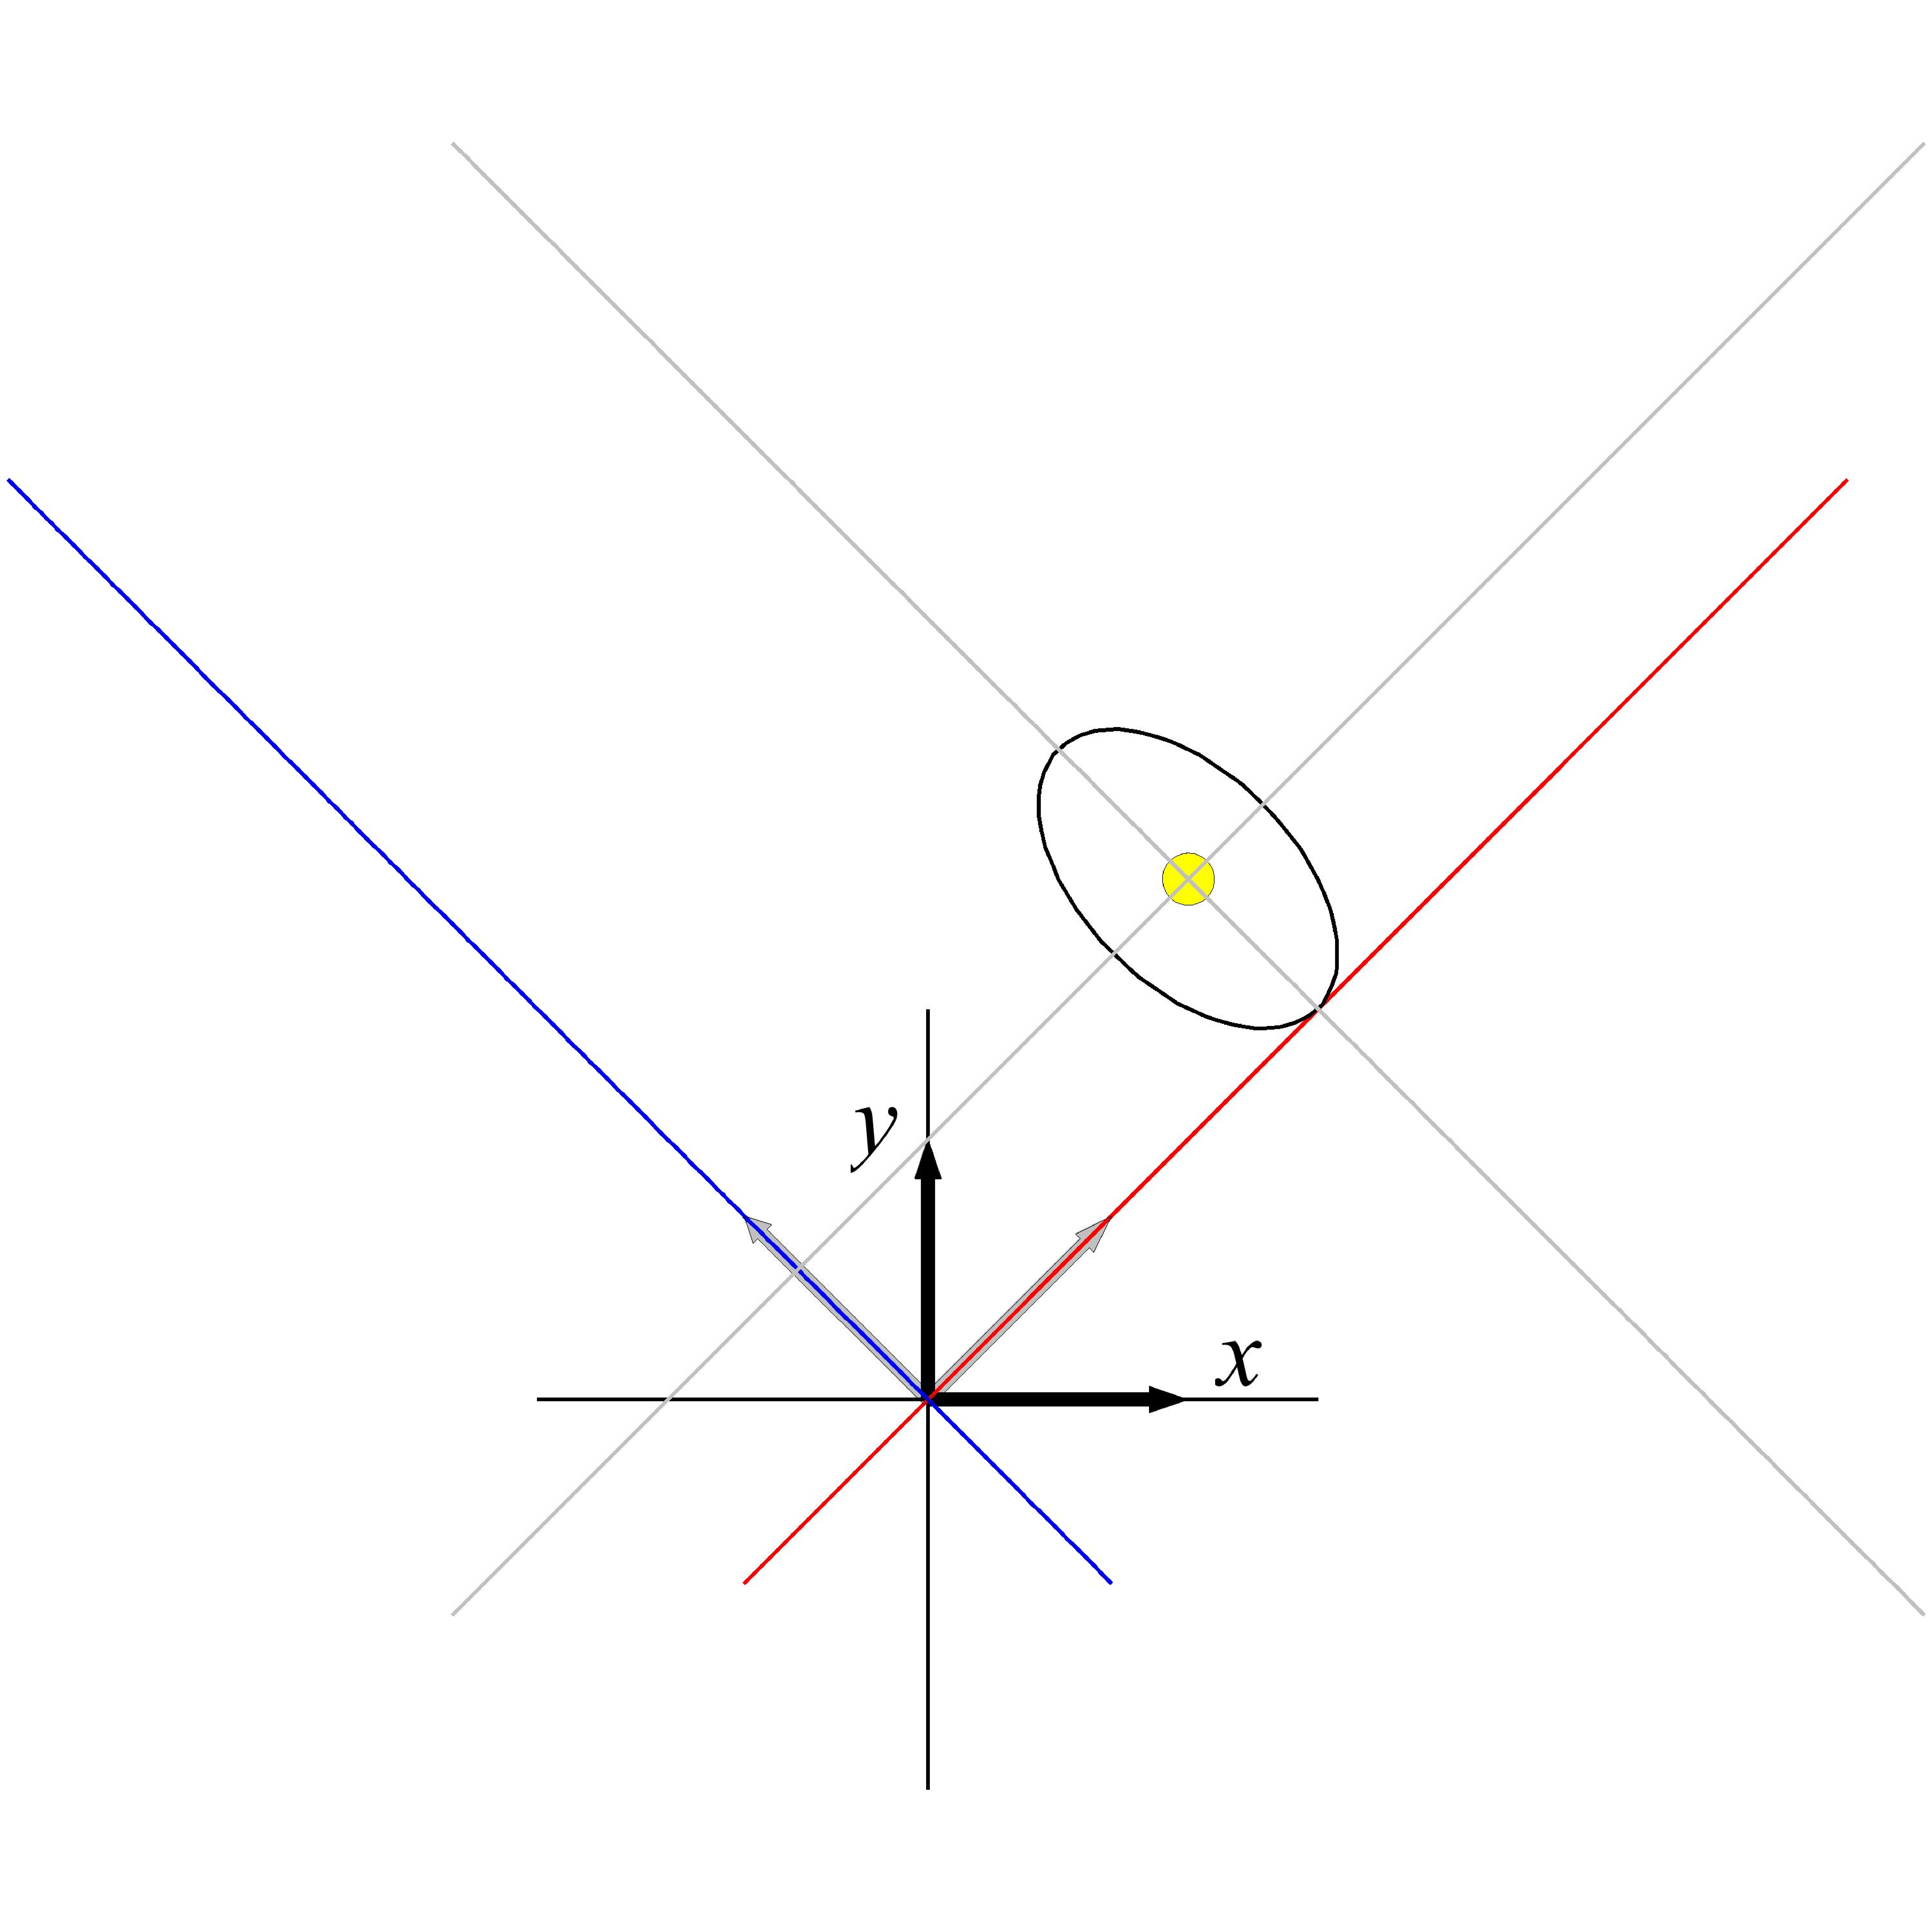
\includegraphics[height=60mm]{FIGS/plotEllipKvad02.pdf}}
\begin{center}
\caption{Grafen for den funktion, der blot er løftet $1/2$ i forhold til værdierne for funktionen i eksempel \ref{exampEllip01}. Niveaukurven $\mathcal{K}_{0}(f)$ i niveau $0$ er tilsvarende \emph{mindre} med tilsvarende mindre halvakser, men den er orienteret efter de samme akseretninger.} \label{figEllip02Kvad}
\end{center}
\end{figure}




\begin{example}[Ellipse] \label{exampEllip02}
\begin{equation}
\begin{aligned}
f(x,y) &= 29\cdot x^{2} + 36\cdot y^{2} + 24\cdot x \cdot y - 152\cdot x -336\cdot y + 620 \quad . \\   \\
\bm{\nabla}f(x,y) &= (58\cdot x + 24 \cdot y -152\, , \, 72\cdot y + 24 \cdot x - 336)  \quad . \\   \\
\frac{1}{2}\cdot \mathbf{H}f(x,y) &= \left[
                     \begin{array}{cc}
                       29 & 12 \\
                       12 & 36 \\
                     \end{array}
                   \right] \quad . \\  \\
\bm{\Lambda} &= \left[
                     \begin{array}{cc}
                       45 & 0 \\
                       0 & 20 \\
                     \end{array}
                   \right]\quad . \\   \\
\mathbf{Q} &= \left[
                     \begin{array}{cc}
                       3/5 & -4/5 \\
                       4/5 & 3/5 \\
                     \end{array}
                   \right]  \quad . \\  \\
\widetilde{f}(\widetilde{x}, \widetilde{y}) & =  45 \cdot \widetilde{x}^{2} + 20 \cdot \widetilde{y}^{2} - 360\cdot \widetilde{x} - 80\cdot \widetilde{y} + 620 \\
&= 45\cdot\left( \widetilde{x} - 4 \right)^{2} + 20\cdot\left(\widetilde{y} - 2 \right)^{2} - 180  \quad. \\
\end{aligned}
\end{equation}
Den andengradsligning som giver niveaukurven $\mathcal{K}_{0}(f)$ er derfor givet ved hver enkelt af følgende ækvivalente ligninger:
\begin{equation}
\begin{aligned}
f(x,y) &= 0 =
\widetilde{f}(\widetilde{x}, \widetilde{y}) \\
\left(\frac{ \widetilde{x} - 4}{2} \right)^{2} &+ \left(\frac{\widetilde{y} - 2 }{3}\right)^{2} = 1 \quad . \\
\end{aligned}
\end{equation}
Dette er ligningen for en \emph{ellipse} med centrum i $\vekind{e}{\mathbf{C}} = (x_{0}, y_{0}) =  (4/5, 22/5)$ (med hensyn til de gamle koordinater) svarende til
$\vekind{v}{\mathbf{C}} = (\widetilde{x}_{0}, \widetilde{y}_{0}) =  (4, 2 )$ (med hensyn til de nye koordinater)  og halvakserne $2$ og $3$, se figur \ref{figEllipKvadBig}. Det nye koordinatsystem fremkommer ved drejning af det gamle koordinatsystem med drejningsvinklen $\phi = \arccos(3/5)$.\\

Andengradspolynomiet $f(x,y)$ har et stationært punkt i centrum med værdien $-180$. Hesse-matricen er positiv definit og derfor er det stationære punkt et egentligt lokalt minimumpunkt  med minimumværdi $-180$. Der er igen tydeligvis tale om et globalt minimumpunkt.
\end{example}



\begin{figure}[ht]
\centerline{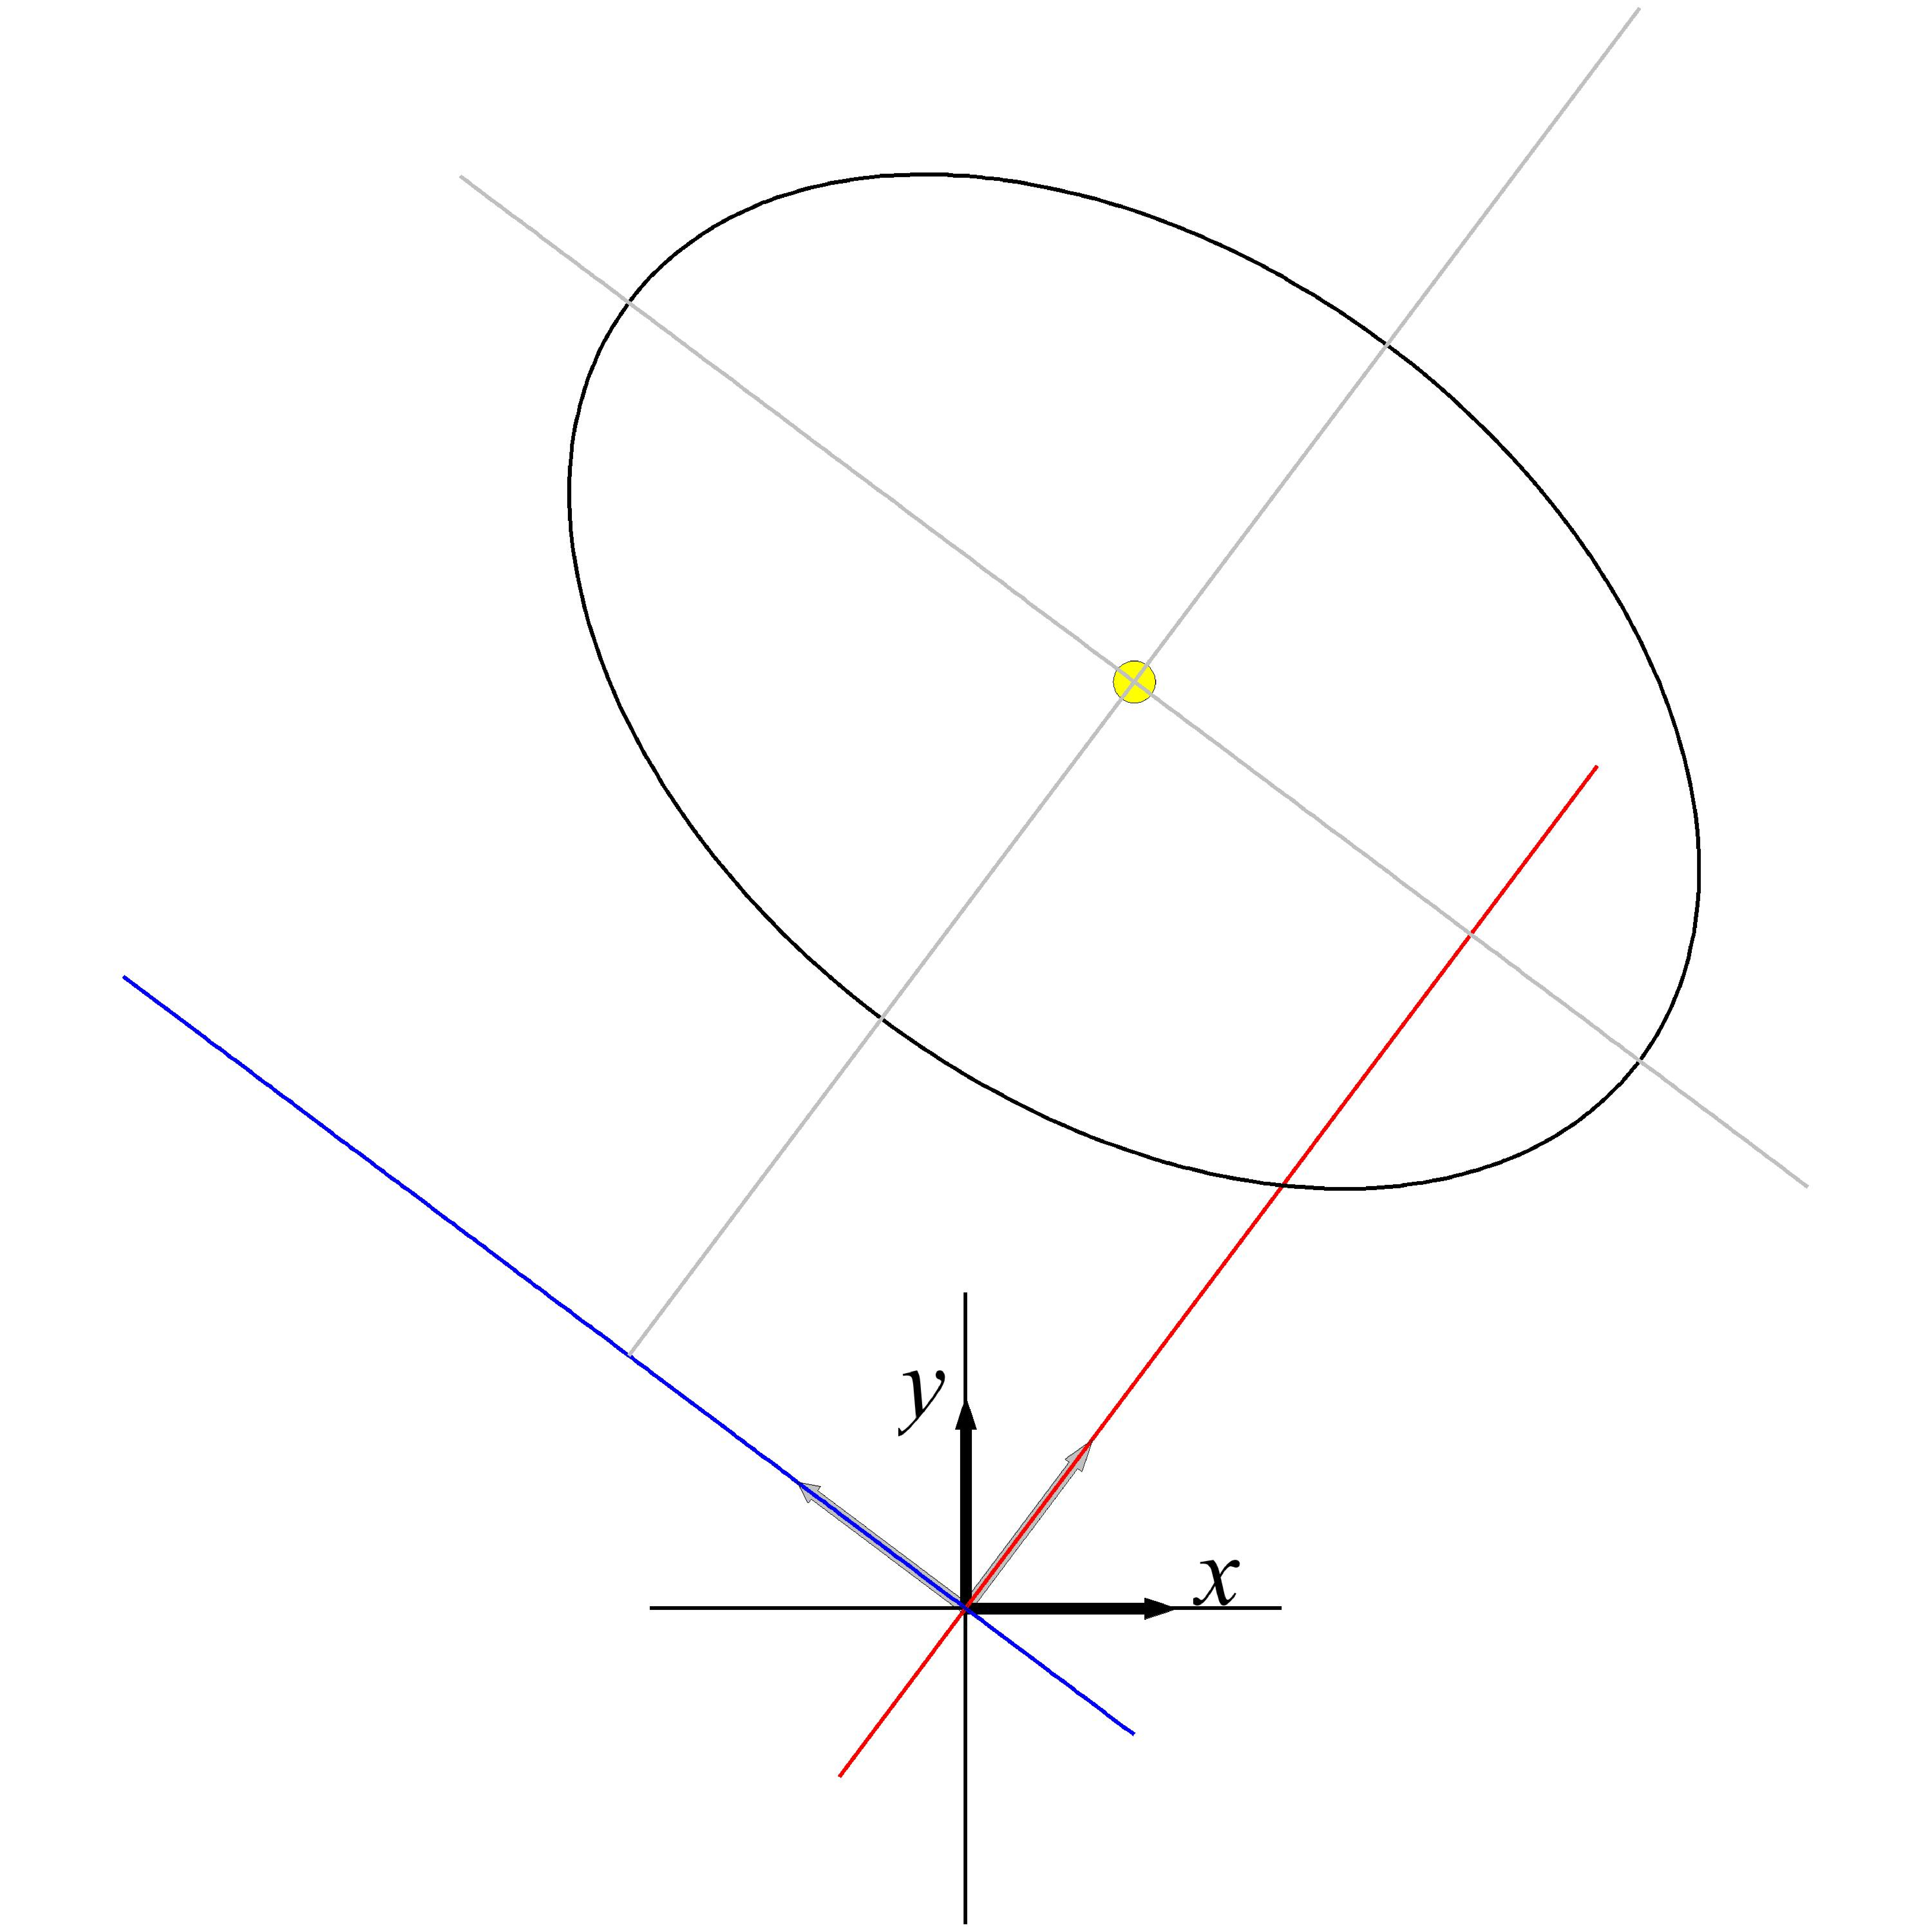
\includegraphics[height=60mm]{FIGS/plotEllipKvadBig.pdf}}
\begin{center}
\caption{Niveaukurven $\mathcal{K}_{0}(f)$ for andengradspolynomiet  $f(x,y) = 29\cdot x^{2} + 36\cdot y^{2} + 24\cdot x \cdot y - 152\cdot x -336\cdot y + 620$ fra eksempel \ref{exampEllip02}.} \label{figEllipKvadBig}
\end{center}
\end{figure}
%%%%%%%%%%%%%%%%%%%%%%%%%%%%%%%%%%%%%%%%%%%%%%%%%%%%%%%%%%%%%
%%%%%%%%%%%%%%%%%%%%%%%%%%%%%%%%%%%%%%%%%%%%%%%%%%%%%%%%%%%%%
%%%%%%%%%%%%%%%%%%%%%%%%%%%%%%%%%%%%%%%%%%%%%%%%%%%%%%%%%%%%%



\begin{example}[Hyperbel] \label{exampHyp02}
Vi ser igen  på \tref{NUID34-exampRedPoly1}{eksempel} fra  \tref{NUID34-tn19}{eNote} som handler om andengradspolynomiet $f(x,y)$ med følgende data:
\begin{equation}
\begin{aligned}
f(x,y) &= 11\cdot x^{2} + 4\cdot y^{2} - 24\cdot x\cdot y - 20\cdot x + 40\cdot y - 60 \quad . \\   \\
\bm{\nabla}f(x,y) &= (22\cdot x - 24 \cdot y - 20\, , \, -24\cdot x + 8\cdot y + 40) \quad . \\  \\
\frac{1}{2}\cdot \mathbf{H}f(x,y) &= \left[
               \begin{array}{cc}
                 11 & -12 \\
                 -12 & 4 \\
               \end{array}
             \right] \quad . \\  \\
\bm{\Lambda} &= \left[
                     \begin{array}{cc}
                       20 & 0 \\
                       0 & -5 \\
                     \end{array}
                   \right] \quad . \\  \\
\mathbf{Q}&= \left[
              \begin{array}{cc}
                4/5 & 3/5 \\
                -3/5 & 4/5 \\
              \end{array}
            \right]  = \left[
                         \begin{array}{cc}
                           \cos(\varphi) & - \sin(\varphi) \\
                           \sin(\varphi) & \cos(\varphi) \\
                         \end{array}
                       \right] \quad , \quad  \textrm{hvor}\quad \varphi = -\arcsin(3/5) \quad . \\   \\
\widetilde{f}(\widetilde{x}, \widetilde{y}) & = 20\cdot  \widetilde{x}^{2} - 5\cdot \widetilde{y}^{2}-40 \cdot \widetilde{x} + 20\cdot \widetilde{y} -60\\
&= 20\cdot (\widetilde{x}-1)^{2} - 5\cdot (\widetilde{y}-2)^{2} -60 \quad. \\
\end{aligned}
\end{equation}
Den andengradsligning som giver niveaukurven $\mathcal{K}_{0}(f)$ er derfor givet ved hver af følgende ligninger:
\begin{equation}
\begin{aligned}
f(x,y) &= 0 =
\widetilde{f}(\widetilde{x}, \widetilde{y})\\
\left(\frac{\widetilde{x}-1}{\sqrt{3}}\right)^{2} &- \left(\frac{\widetilde{y}- 2}{2\cdot\sqrt{3}} \right)^{2} = 1 \quad . \\
\end{aligned}
\end{equation}
Ligningerne fremstiller en \emph{hyperbel} med centrum i $\vekind{e}{\mathbf{C}} = (x_{0}, y_{0}) =  (2,1)$ (med hensyn til de gamle koordinater) svarende til
$\vekind{v}{\mathbf{C}} = (\widetilde{x}_{0}, \widetilde{y}_{0}) = (1, 2)$ (med hensyn til de nye koordinater)  og halvakserne $\sqrt{3}$ og $2\cdot\sqrt{3}$. Det nye koordinatsystem fremkommer ved drejning af det gamle koordinatsystem med drejningsvinklen $\phi = -\arcsin(3/5)$.\\

Funktionen har et stationært punkt i centrum med værdien $-60$. Hesse-matricen er indefinit og derfor er det stationære punkt hverken et lokalt minimumpunkt eller maksimumpunkt.
\end{example}




%%%%%%%%%%%%%%%%%%%%%%%%%%%%%%%%%%%%%%%%%%%%%%%%%%%%%%%%%%%%%
%%%%%%%%%%%%%%%%%%%%%%%%%%%%%%%%%%%%%%%%%%%%%%%%%%%%%%%%%%%%%
%%%%%%%%%%%%%%%%%%%%%%%%%%%%%%%%%%%%%%%%%%%%%%%%%%%%%%%%%%%%%



\begin{example}[Hyperbel] \label{exampHyp01}
En anden hyperbel er givet ved $\mathcal{K}_{0}(f)$ for følgende andengradspolynomium:
\begin{equation}
\begin{aligned}
f(x,y) &= -\frac{5}{4}\cdot x^{2} + \frac{1}{4}\cdot y^{2} + \frac{3}{2}\cdot \sqrt{3}\cdot x \cdot y + 5\cdot x -3\cdot \sqrt{3}\cdot y  -\frac{21}{4} \quad . \\   \\
\bm{\nabla}f(x,y) &= (-\frac{5}{2}\cdot x  + \frac{3}{2}\cdot \sqrt{3}\cdot y + 5\, , \, \frac{3}{2}\cdot \sqrt{3} \cdot x + \frac{1}{2}\cdot y - 3 \cdot \sqrt{3}) \quad . \\   \\
\frac{1}{2}\cdot \mathbf{H}f(x,y) &= \left[
                     \begin{array}{cc}
                       -5/2 & 3\cdot \sqrt{3}/4 \\
                       \sqrt{3}/4 & 1/4 \\
                     \end{array}
                   \right] \quad . \\  \\
\bm{\Lambda} &= \left[
                     \begin{array}{cc}
                       1 & 0 \\
                       0 & -2 \\
                     \end{array}
                   \right] \quad . \\  \\
\mathbf{Q} &= \left[
                     \begin{array}{cc}
                       1/2 & -\sqrt{3}/2 \\
                       \sqrt{3}/2 & 1/2 \\
                     \end{array}
                   \right] = \left[
                     \begin{array}{cc}
                       \cos(\pi/3) & -\sin(\pi/3) \\
                        \sin(\pi/3) &  \cos(\pi/3)\\
                     \end{array}
                   \right] \quad . \\  \\
\widetilde{f}(\widetilde{x}, \widetilde{y}) & =  \widetilde{x}^{2} - 2\cdot \widetilde{y}^{2} - 2 \cdot \widetilde{x} - 4\cdot \sqrt{3}\cdot \widetilde{y} - \frac{21}{4}\\
&= (\widetilde{x}-1)^{2} - 2\cdot (\widetilde{y}+ \sqrt{3})^{2} - \frac{1}{4} \quad.
\end{aligned}
\end{equation}
Den andengradsligning som giver niveaukurven $\mathcal{K}_{0}(f)$ er derfor givet ved hver af følgende ækvivalente ligninger, hvor den sidste fås ved kvadratkomplettering:
\begin{equation}
\begin{aligned}
f(x,y) &= 0 =
\widetilde{f}(\widetilde{x}, \widetilde{y}) = 0 \\
\left(\frac{\widetilde{x}-1}{\frac{1}{2}}\right)^{2} &- \left(\frac{\widetilde{y}+ \sqrt{3}}{\frac{1}{2\cdot \sqrt{2}}} \right)^{2} = 1 \quad . \\
\end{aligned}
\end{equation}
Det er en \emph{hyperbel} med centrum i $\vekind{e}{\mathbf{C}} = (x_{0}, y_{0}) =  (2,0)$ (med hensyn til de gamle koordinater) svarende til
$\vekind{v}{\mathbf{C}} = (\widetilde{x}_{0}, \widetilde{y}_{0}) = (1, -\sqrt{3} )$ (med hensyn til de nye koordinater)  og halvakserne $1/2$ og $1/(2\cdot \sqrt{2})$, se figur \ref{figHyp01Kvad}. Det nye koordinatsystem fremkommer ved drejning af det gamle koordinatsystem med drejningsvinklen $\phi = \frac{\pi}{3}$.\\

Funktionen har et stationært punkt i centrum med værdien $-1/4$. Hesse-matricen er indefinit og derfor er det stationære punkt hverken et lokalt minimumpunkt eller maksimumpunkt, som det også tydeligt fremgår af figur \ref{figHyp01Kvad}.
\end{example}



\begin{figure}[ht]
\centerline{  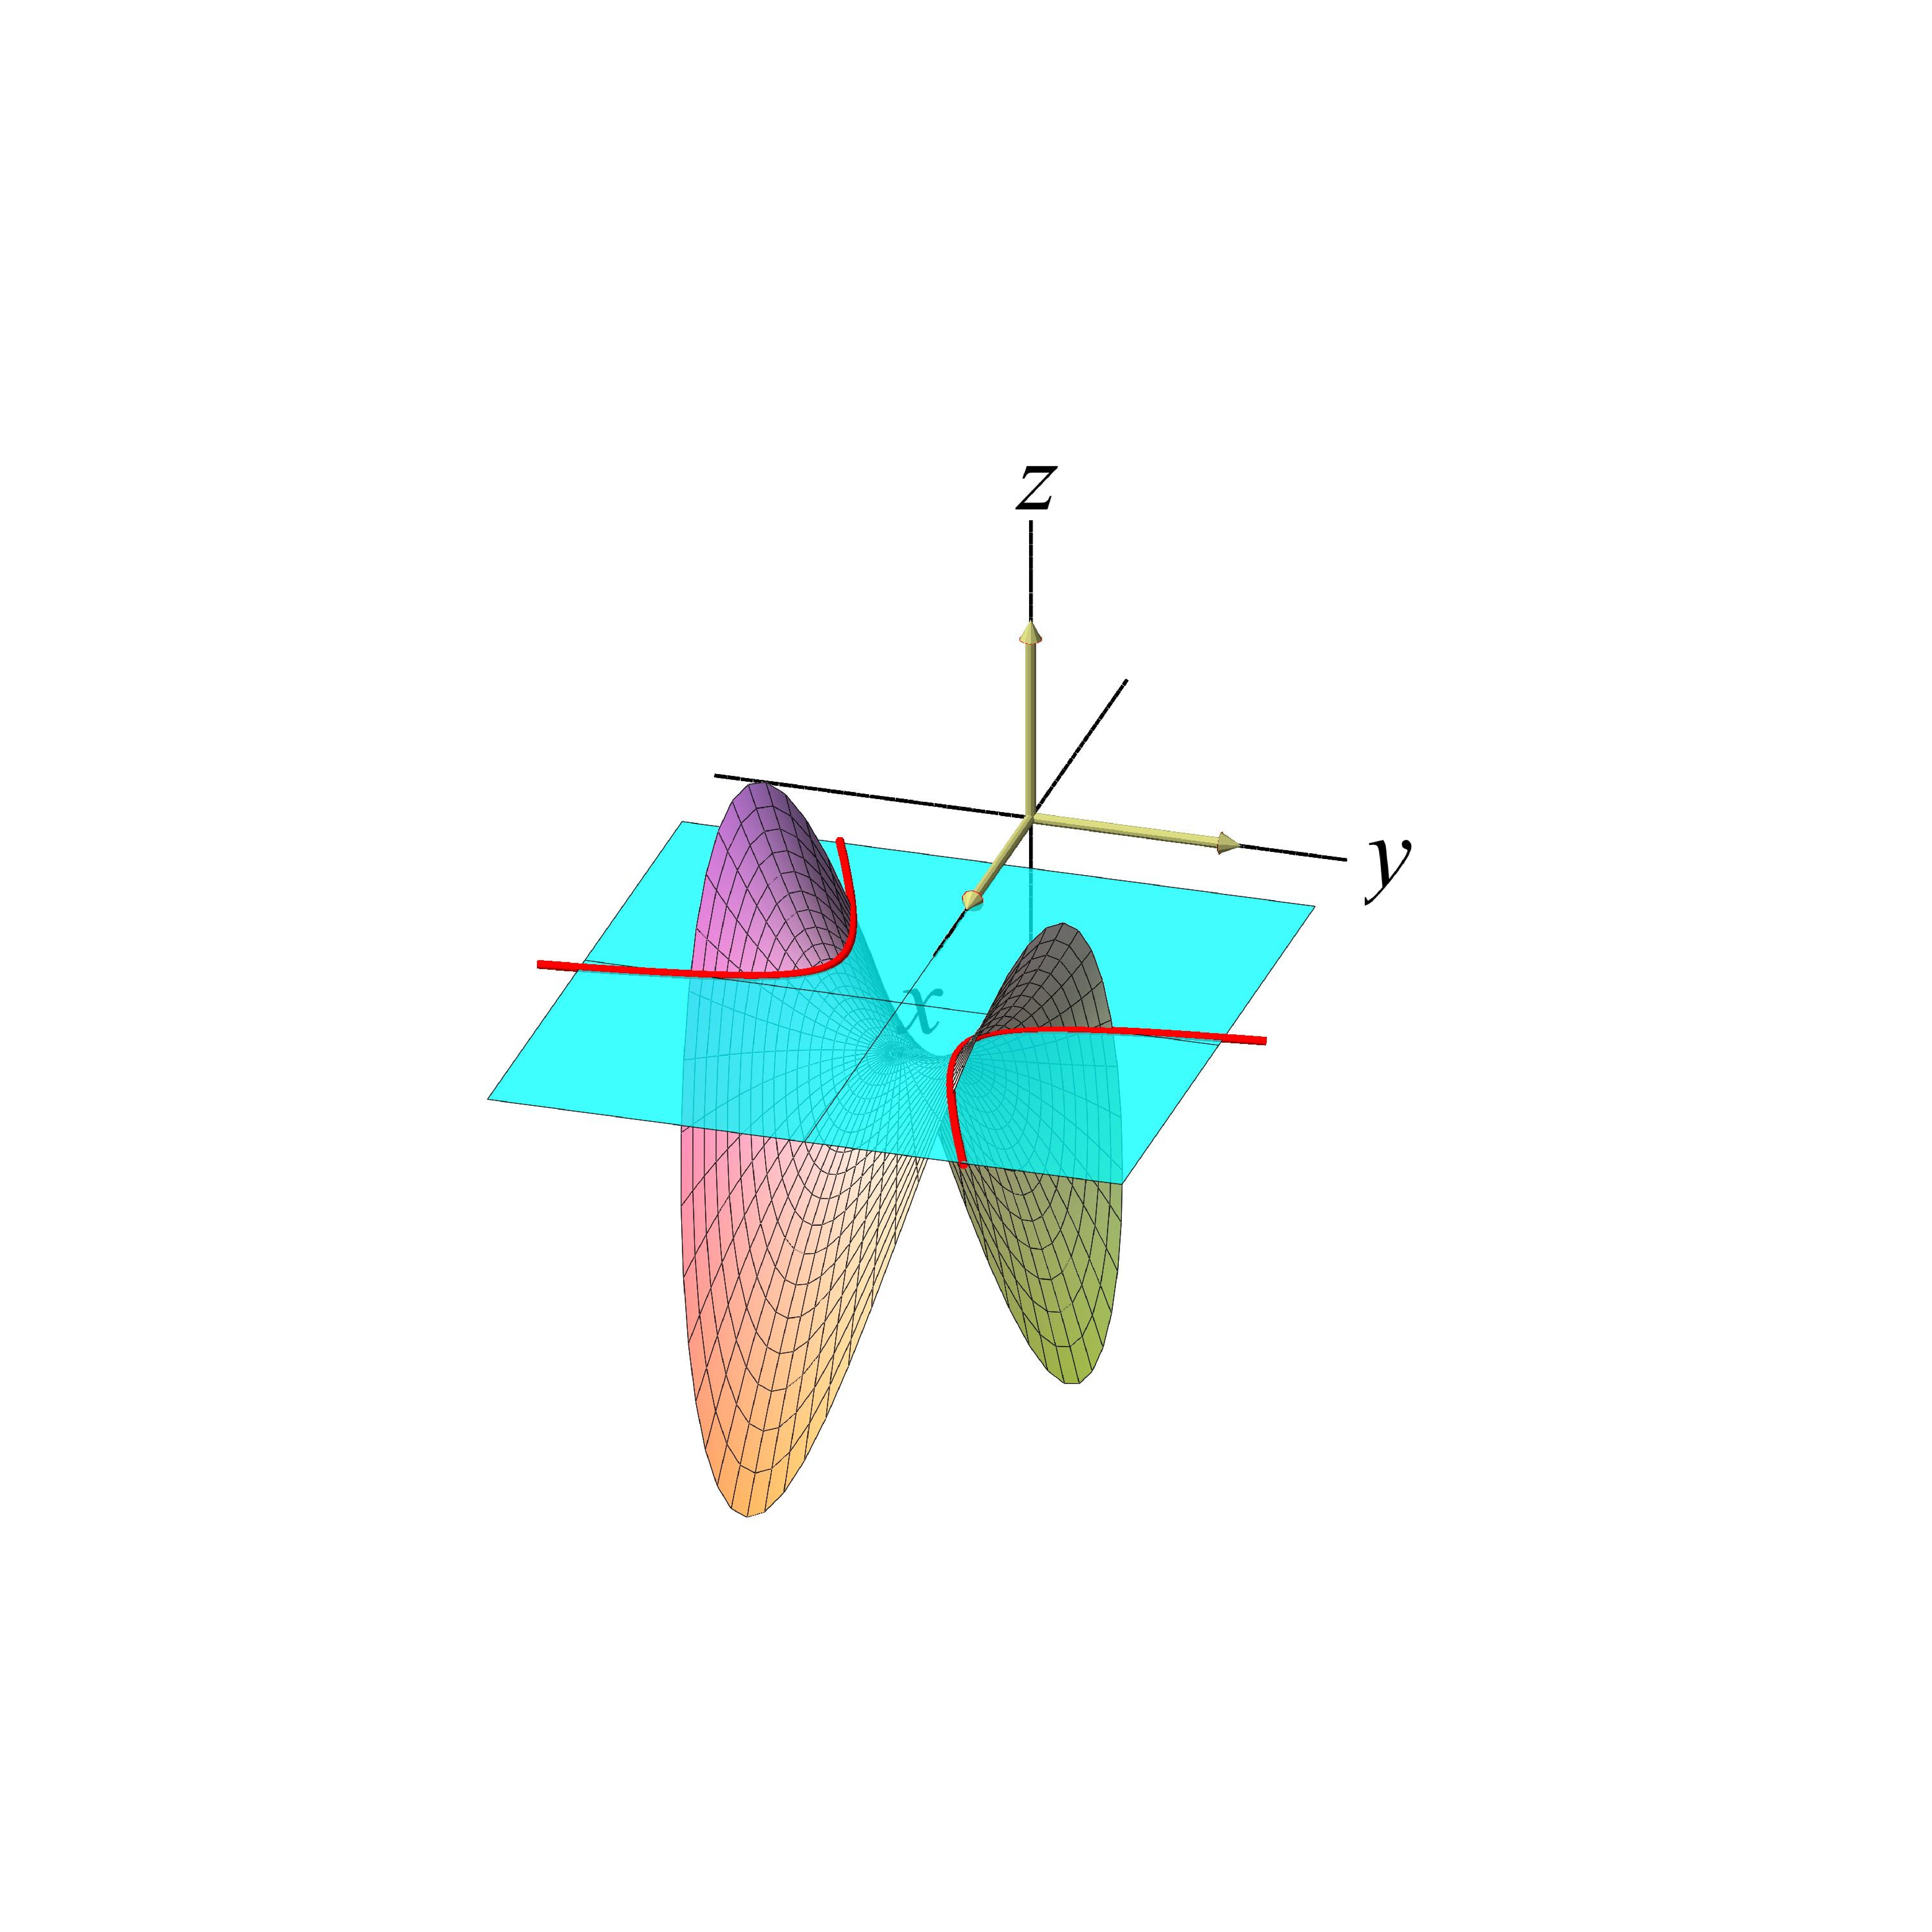
\includegraphics[height=60mm]{FIGS/plot2DNivHypLift01.pdf} 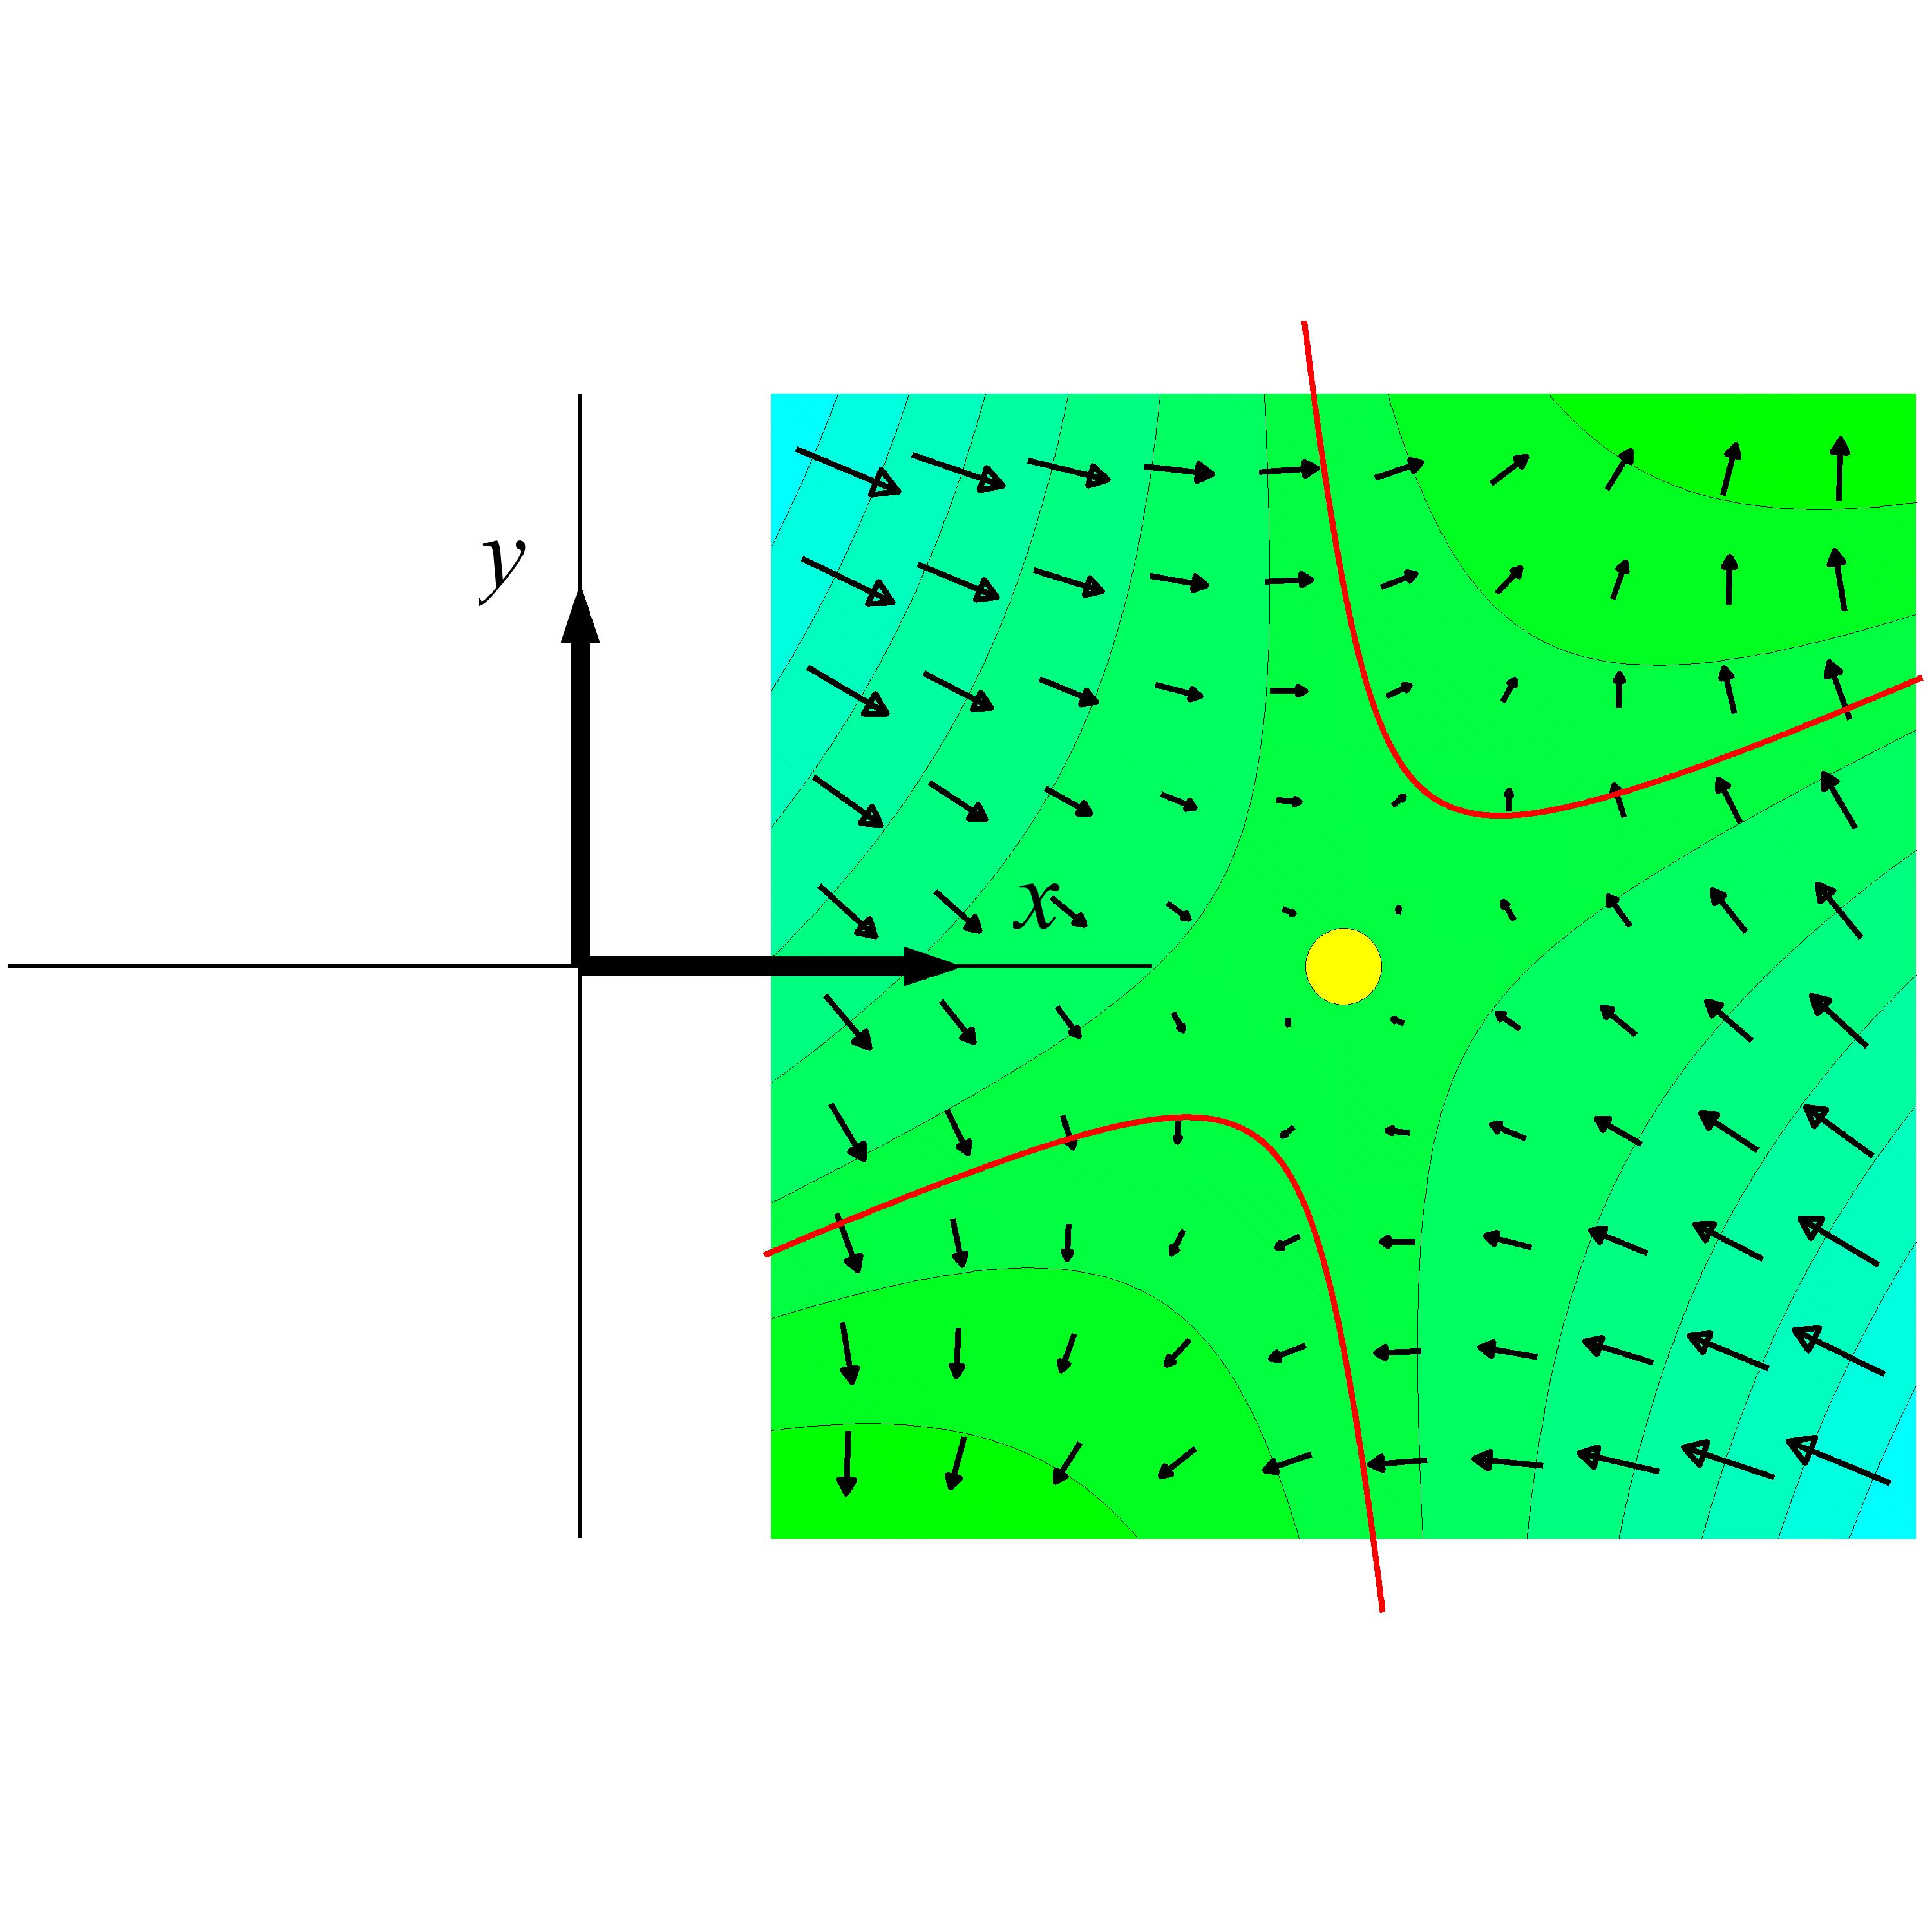
\includegraphics[height=60mm]{FIGS/plot2DGradHyp01.pdf} 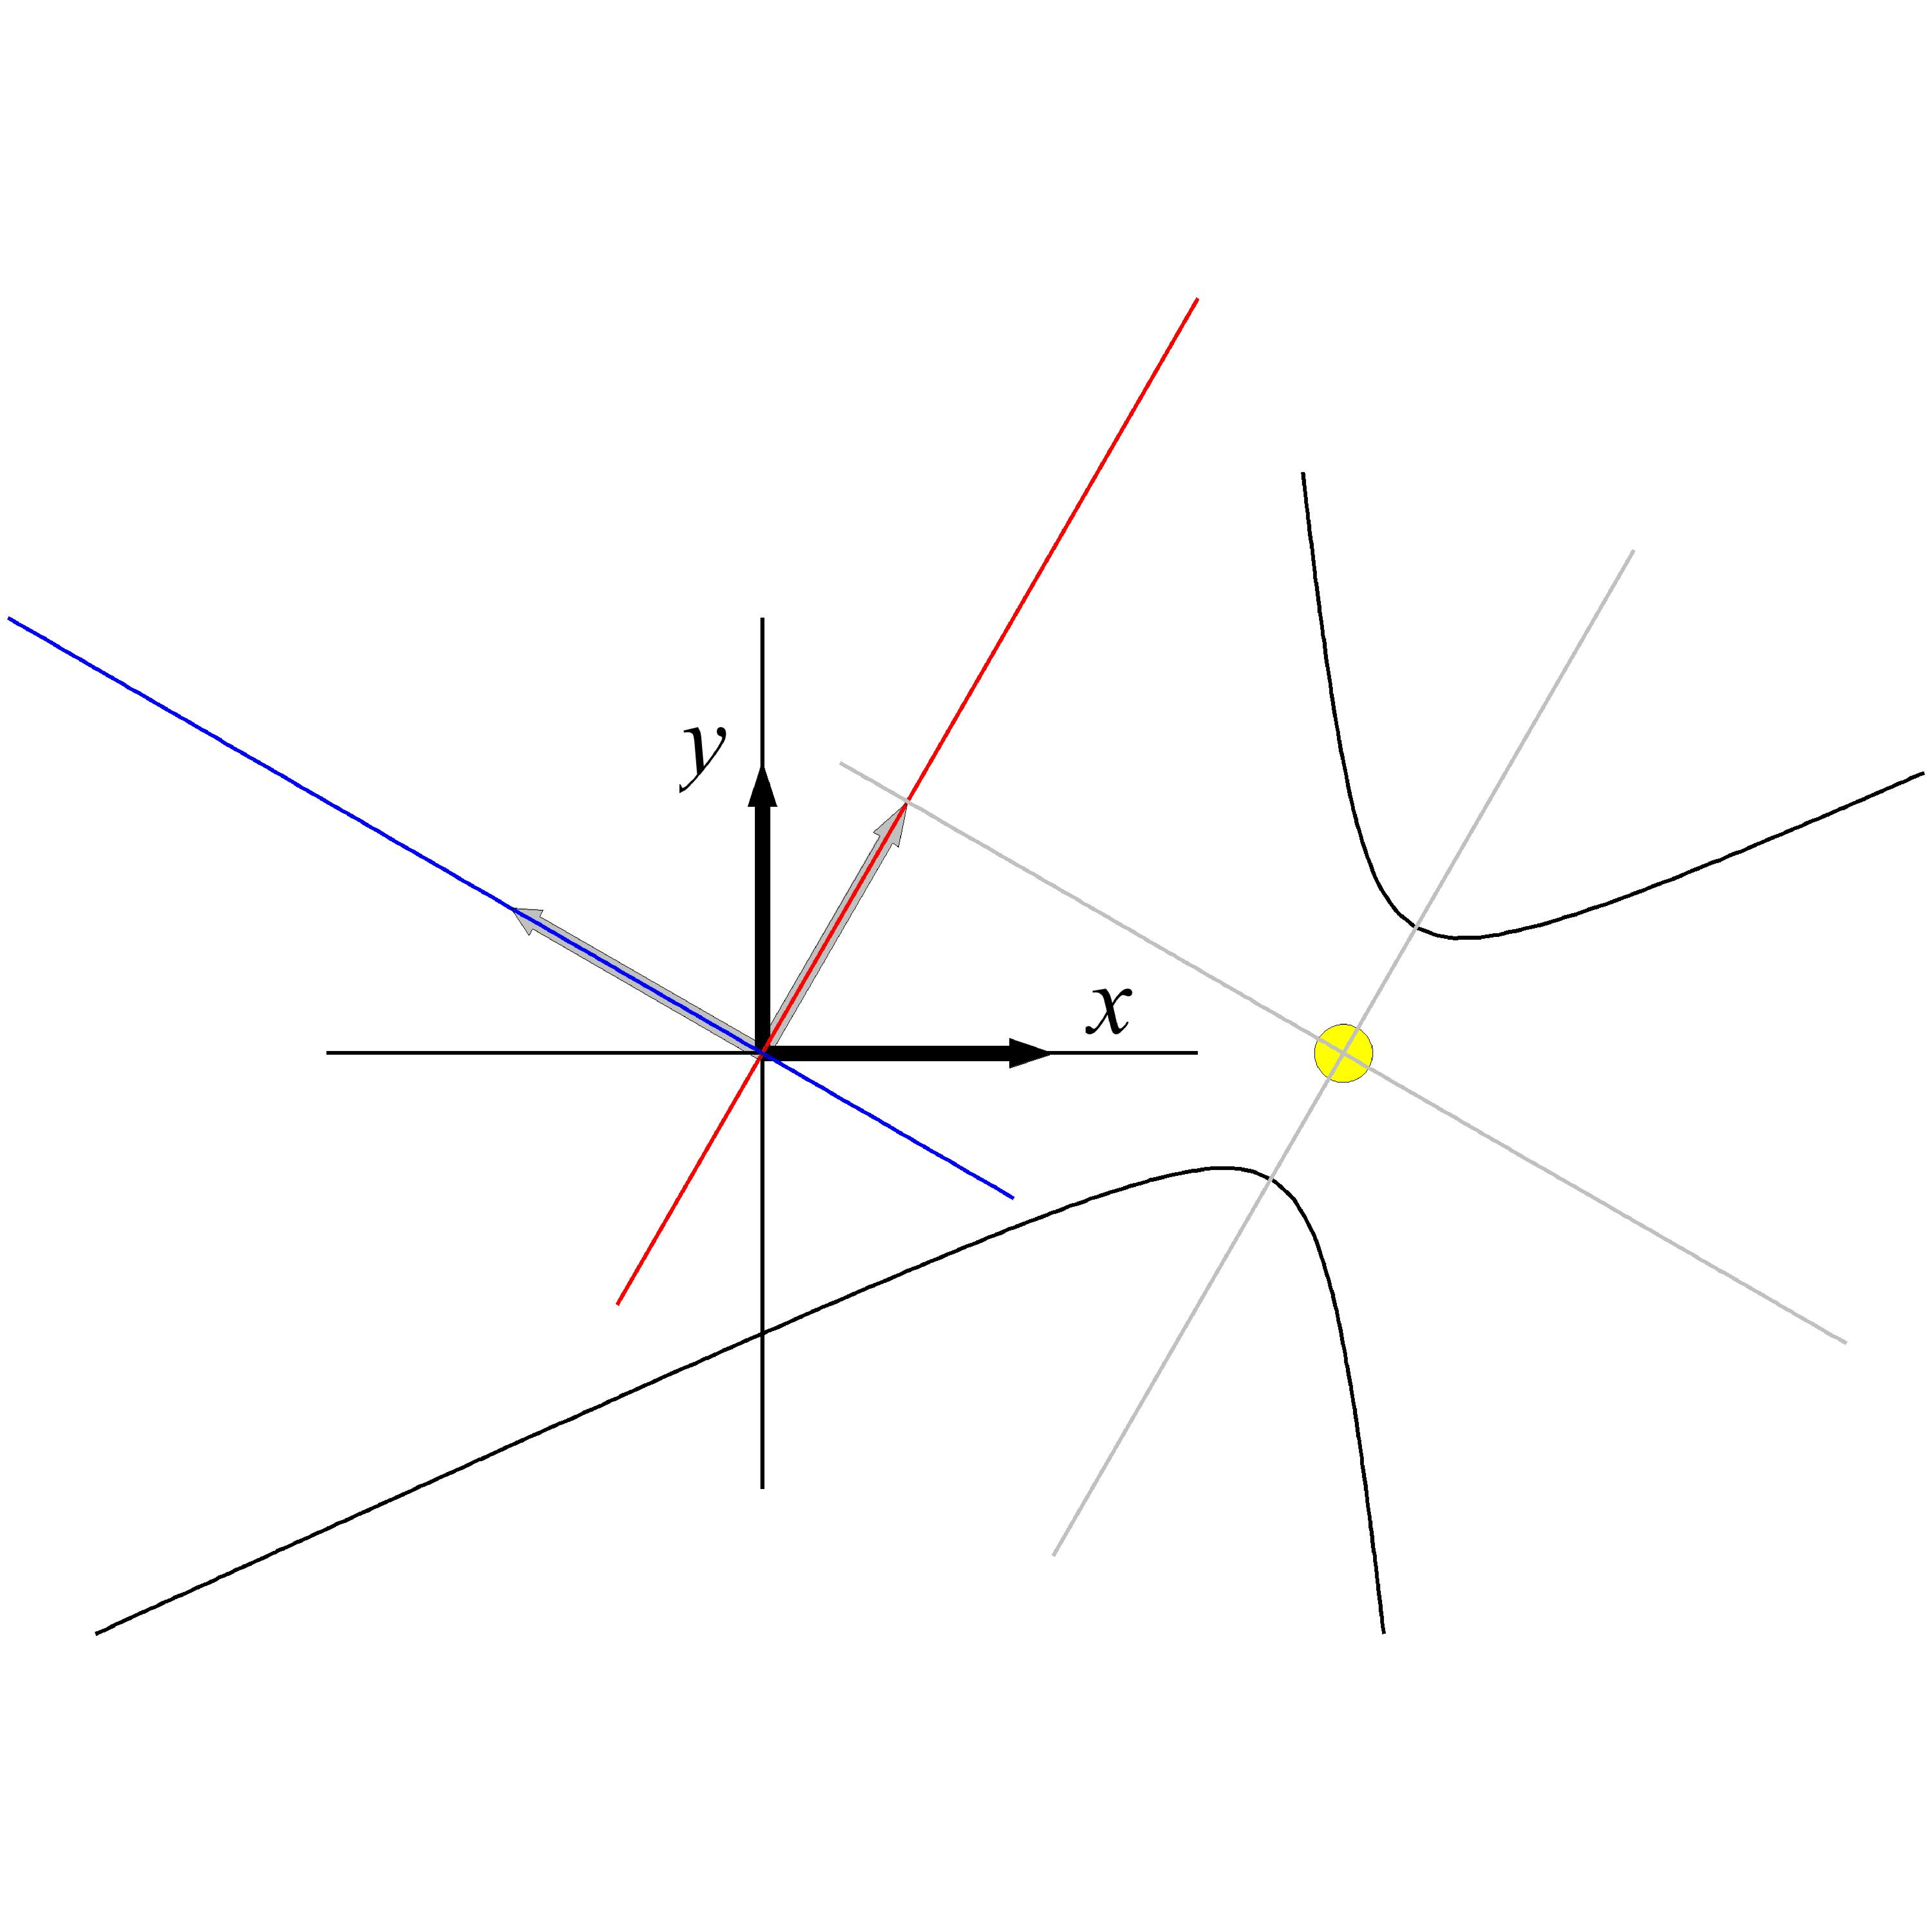
\includegraphics[height=60mm]{FIGS/plotHypKvad01.pdf}}
\begin{center}
\caption{Grafen for funktionen fra eksempel \ref{exampHyp01} med snit i niveau $0$, gradientfelt, niveaukurver og specielt niveaukurven $\mathcal{K}_{0}(f)$.} \label{figHyp01Kvad}
\end{center}
\end{figure}




%%%%%%%%%%%%%%%%%%%%%%%%%%%%%%%%%%%%%%%%%%%%%%%%%%%
%%%%%%%%%%%%%%%%%%%%%%%%%%%%%%%%%%%%%%%%%%%%%%%%%%%
%%%%%%%%%%%%%%%%%%%%%%%%%%%%%%%%%%%%%%%%%%%%%%%%%%%

\section{Andengradsligninger i tre variable} \label{chpSymmMat}

For andengradspolynomier $f(x,y,z)$ i tre variable kan vi gennemføre samme analyse som ovenfpor men nu af de niveaumængder i rummet, dvs. de niveau-flader der fremkommer ved at sætte $f(x,y, z)=0$. Vi viser metoden via nogle eksempler:

\begin{example}[Ellipsoide] \label{exampEllip3D01}
Et andengradspolynomium i tre variable undersøges:
\begin{equation}
\begin{aligned}
f(x,y,z) &= 7\cdot x^{2} + 6\cdot y^{2} + 5\cdot z^{2} - 4\cdot x\cdot y - 4\cdot y \cdot z  -2\cdot x +20 \cdot y  - 10\cdot z + 15 \quad . \\   \\
\bm{\nabla}f(x,y,z) &= (14\cdot x -4\cdot y-2, -4\cdot x + 12\cdot y - 4 \cdot z +20, -4\cdot y + 10\cdot z -10  ) \quad . \\  \\
\frac{1}{2}\cdot \mathbf{H}f(x,y,z) &= \left[
                     \begin{array}{ccc}
                       7 & -2 & 0\\
                       -2 & 6 & -2 \\
                       0 & -2 & 5\\
                     \end{array}
                   \right] \quad . \\  \\
\bm{\Lambda} &= \left[
                     \begin{array}{ccc}
                       9 & 0 & 0 \\
                       0 & 6 & 0 \\
                       0 & 0 & 3 \\
                     \end{array}
                   \right] \quad . \\  \\
\mathbf{Q} &= \left[
                     \begin{array}{ccc}
                       2/3 & -2/3 & -1/3 \\
                      -2/3& -1/3& -2/3\\
                       1/3 & 2/3 & -2/3\\
                     \end{array}
                   \right]\quad . \\  \\
\widetilde{f}(\widetilde{x}, \widetilde{y}, \widetilde{z}) & = 9\cdot \widetilde{x}^{2} + 6\cdot \widetilde{y}^{2} + 3 \cdot \widetilde{z}^{2} -18\cdot \widetilde{x} - 12\cdot \widetilde{y} -6\cdot \widetilde{z} +15 \\
&= 9\cdot\left(\widetilde{x} - 1\right)^{2} + 6\cdot\left(\widetilde{y} - 1 \right)^{2} + 3\cdot \left(\widetilde{z} - 1 \right)^{2}-3 \quad.
\end{aligned}
\end{equation}
Den andengradsligning som giver niveaufladen $\mathcal{K}_{0}(f)$ er derfor givet ved hver af følgende ækvivalente ligninger:
\begin{equation}
\begin{aligned}
f(x,y,z) &= 0 =
\widetilde{f}(\widetilde{x}, \widetilde{y}, \widetilde{z})  \\
\left(\frac{\widetilde{x} - 1}{\frac{1}{\sqrt{3}}}\right)^{2} &+ \left(\frac{\widetilde{y} - 1}{\frac{1}{\sqrt{2}}}\right)^{2} +  \left(\widetilde{z} - 1\right)^{2} = 1 \quad .
\end{aligned}
\end{equation}
Det er ligningen for en \emph{ellipsoide} med centrum i $\vekind{e}{\mathbf{C}} = (x_{0}, y_{0}, z_{0}) =  (-1/3, -5/3, 173)$ (med hensyn til de gamle koordinater) svarende til
$\vekind{v}{\mathbf{C}} = (\widetilde{x}_{0}, \widetilde{y}_{0}, \widetilde{z}_{0}) =  (1,1,1)$ (med hensyn til de nye koordinater)  og halvakserne $\frac{1}{\sqrt{3}}$ og $\frac{1}{\sqrt{2}}$, og $1$, se figur \ref{figEllip3D01Kvad} og navnetabellen i afsnit \ref{secNavnetabel}. Det nye koordinatsystem fremkommer ved rotation af det gamle koordinatsystem med den positive ortogonale substitution  $\mathbf{Q}$.
\end{example}



\begin{figure}[ht]
\centerline{  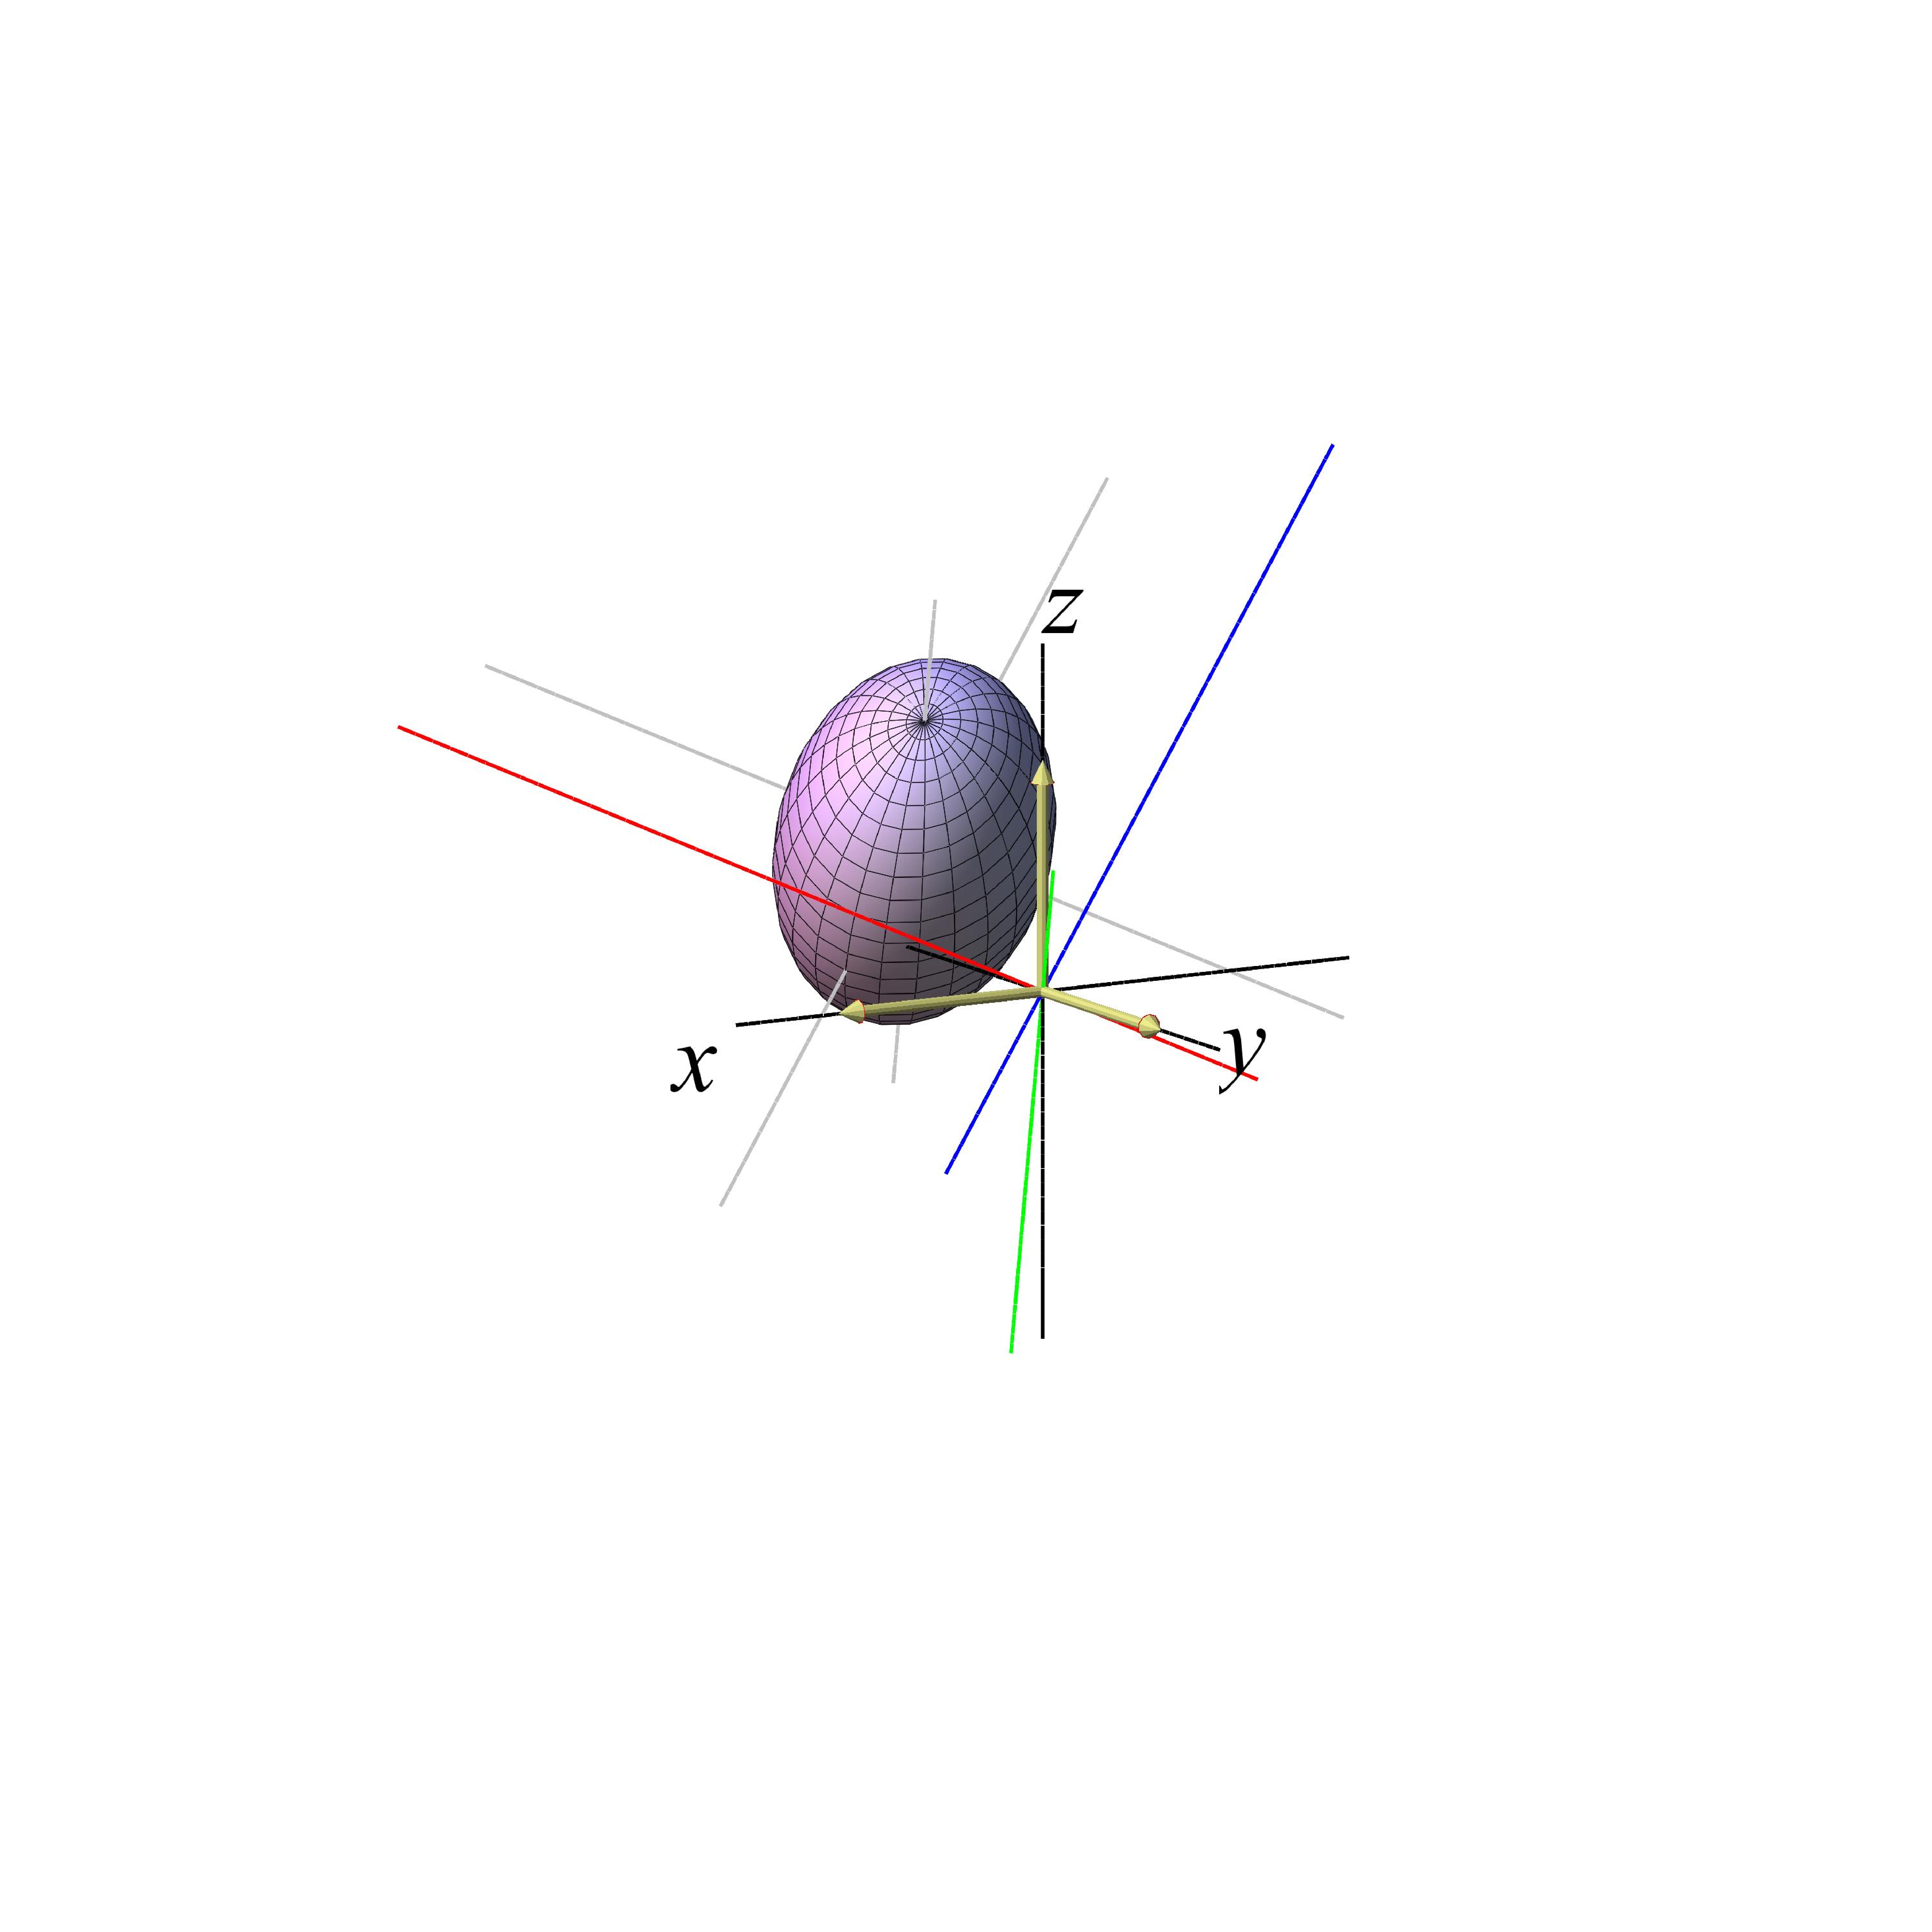
\includegraphics[height=80mm]{FIGS/plotEllip3D01Kvad.pdf}}
\begin{center}
\caption{Niveaufladen $\mathcal{K}_{0}(f)$ for den funktion som er analyseret i eksempel \ref{exampEllip3D01}. Det nye roterede koordinatsystem hvori ellipsoiden har reduceret form er antydet med den røde $\widetilde{x}$-akse, blå $\widetilde{y}$-akse, og grønne $\widetilde{z}$-akse.} \label{figEllip3D01Kvad}
\end{center}
\end{figure}




\begin{think}
Funktionen $f(x,y,z)$, som er undersøgt i eksempel \ref{exampEllip3D01}, har et {\emph{stationært punkt}} i det fundne centrum med værdien $-3$. Hesse-matricen er positiv definit og derfor er det stationære punkt for $f(x,y,z)$ i rummet et egentligt lokalt minimumpunkt, et globalt minimumpunkt.
\end{think}

\begin{aha}
Hvis vi kunne tegne grafen for funktionen $f(x,y,z)$ i det $4$-dimensionale $(x,y,z,w)$-rum, dvs. hvis vi betragtede mængden af de punkter i $\mathbb{R}^{4}$ der kan skrives på formen $(x, y, z, f(x,y,z))$ når $(x,y,z)$ gennemløber $(x,y,z)$-rummet i $\mathbb{R}^{4}$, så vil niveaufladen for $f(x,y,z)$ være den mængde vi får i $(x,y,z)$-rummet  ved at sætte $w=0$, altså netop $f(x,y,z) = 0$.
\end{aha}









%%%%%%%%%%%%%%%%%%%%%%%%%%%%%%%%%%%%%%%%%%%%%%%%%%%%%%%%%%%%%
%%%%%%%%%%%%%%%%%%%%%%%%%%%%%%%%%%%%%%%%%%%%%%%%%%%%%%%%%%%%%
%%%%%%%%%%%%%%%%%%%%%%%%%%%%%%%%%%%%%%%%%%%%%%%%%%%%%%%%%%%%%



\begin{example}[Hyperboloide med \'{e}t net] \label{exampHypEt3D01}
\begin{equation}
\begin{aligned}
f(x,y,z) &= x^{2} + 2\cdot y^{2} + z^{2} + 2\cdot x - 4\cdot y + 2\cdot z - 4 \cdot x \cdot z -1          \quad . \\   \\
\bm{\nabla}f(x,y,z) &= (2\cdot x - 4\cdot z +2, -4\cdot y - 4, -4\cdot x + 2\cdot z  + 2  ) \quad . \\   \\
\frac{1}{2}\cdot \mathbf{H}f(x,y,z) &= \left[
                     \begin{array}{ccc}
                       1 & 0 & -2\\
                       0 & 2 & 0\\
                       -2 & 0 & 1\\
                     \end{array}
                   \right]\quad . \\   \\
\bm{\Lambda} &= \left[
                     \begin{array}{ccc}
                       3 & 0 & 0 \\
                       0 & 2& 0 \\
                       0 & 0 & -1 \\
                     \end{array}
                   \right] \quad . \\  \\
\mathbf{Q} &= \left[
                     \begin{array}{ccc}
                       -\sqrt{2}/2 & 0 & -\sqrt{2}/2 \\
                      0& 1& 0\\
                       \sqrt{2}/2 &0 &  -\sqrt{2}/2\\
                     \end{array}
                   \right] \quad . \\
\end{aligned}
\end{equation}
\begin{equation}
\begin{aligned}
\widetilde{f}(\widetilde{x}, \widetilde{y}, \widetilde{z}) & = 3\cdot \widetilde{x}^{2} + 2\cdot \widetilde{y}^{2} - \widetilde{z}^{2} - 4\cdot \widetilde{y} -2\cdot \sqrt{2} \cdot \widetilde{z} -1 \\
&= 3 \cdot \widetilde{x}^{2} + 2\cdot\left(\widetilde{y} - 1 \right)^{2} - \left(\widetilde{z}+ \sqrt{2} \right)^{2}-1 \quad. \\
\end{aligned}
\end{equation}
Den andengradsligning som giver niveaufladen $\mathcal{K}_{0}(f)$ er derfor givet ved hver af følgende ækvivalente ligninger:
\begin{equation}
\begin{aligned}
f(x,y,z) &= 0=
\widetilde{f}(\widetilde{x}, \widetilde{y}, \widetilde{z}) \\
\left(\frac{\widetilde{x}}{\frac{1}{\sqrt{3}}}\right)^{2} &+ \left(\frac{\widetilde{y} - 1}{\frac{1}{\sqrt{2}}}\right)^{2} -  \left(\widetilde{z} +\sqrt{2}\right)^{2} = 1 \quad .
\end{aligned}
\end{equation}
Ligningerne  repræsenterer en \emph{hyperboloide med \'{e}t net} der har  centrum i $\vekind{e}{\mathbf{C}} = (x_{0}, y_{0}, z_{0}) =  (1,1,1)$ (med hensyn til de gamle koordinater) svarende til
$\vekind{v}{\mathbf{C}} = (\widetilde{x}_{0}, \widetilde{y}_{0}) =  (0, 1, -\sqrt{2})$ (med hensyn til de nye koordinater)  og halvakserne $\frac{1}{\sqrt{3}}$ og $\frac{1}{\sqrt{2}}$, og $1$, se figur \ref{figHypEt3D01Kvad} og navnetabellen i afsnit \ref{secNavnetabel}. Det nye koordinatsystem fremkommer ved rotation af det gamle koordinatsystem med den positive ortogonale substitution  $\mathbf{Q}$.
\end{example}

\begin{think}
Funktionen $f(x,y,z)$, som er undersøgt i eksempel \ref{exampHypEt3D01},  har et {\emph{stationært punkt}} i det fundne centrum med værdien $-1$. Hesse-matricen er indefinit og derfor er det stationære punkt for $f(x,y,z)$ i rummet hverken  minimumpunkt eller maksimumpunkt.
\end{think}




\begin{figure}[ht]
\centerline{  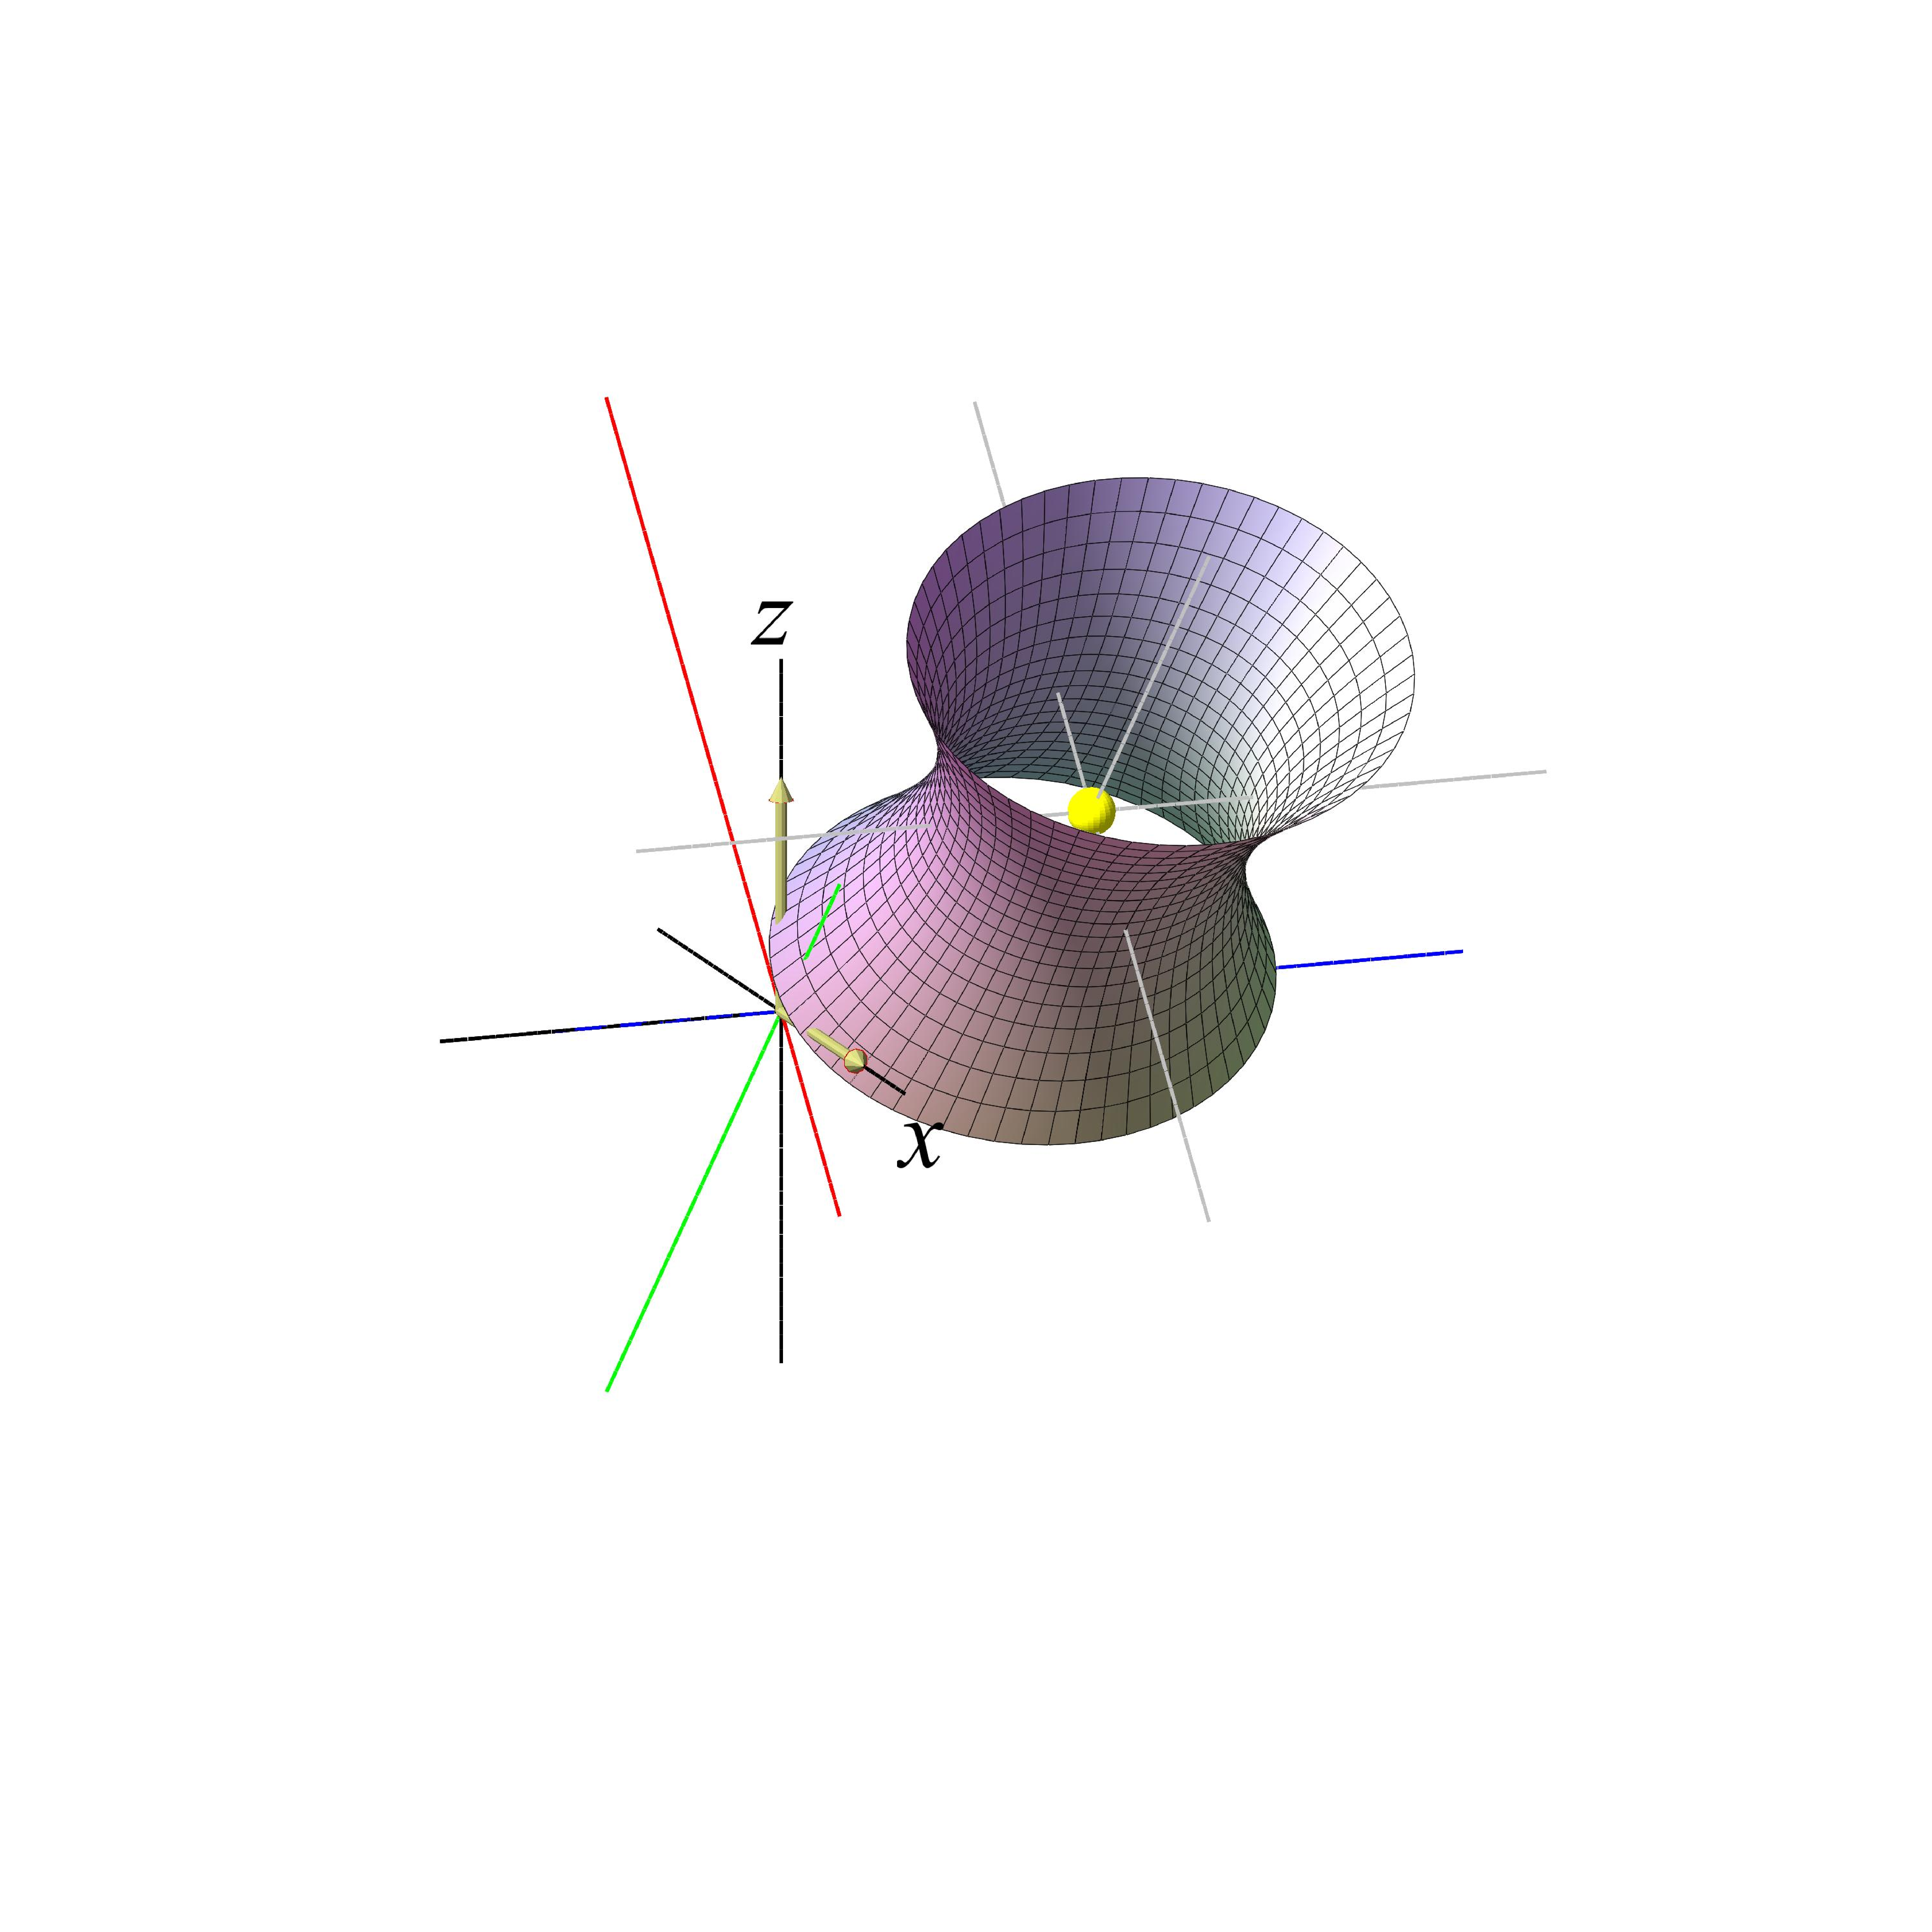
\includegraphics[height=80mm]{FIGS/plotHypEt3D01Kvad.pdf}}
\begin{center}
\caption{Niveaufladen $\mathcal{K}_{0}(f)$ for funktionen som analyseres i eksempel \ref{exampHypEt3D01}.} \label{figHypEt3D01Kvad}
\end{center}
\end{figure}





%%%%%%%%%%%%%%%%%%%%%%%%%%%%%%%%%%%%%%%%%%%%%%%%%%%%%%%%%%%%%
%%%%%%%%%%%%%%%%%%%%%%%%%%%%%%%%%%%%%%%%%%%%%%%%%%%%%%%%%%%%%
%%%%%%%%%%%%%%%%%%%%%%%%%%%%%%%%%%%%%%%%%%%%%%%%%%%%%%%%%%%%%



\begin{example}[Hyperboloide med to net] \label{exampHypTo3D01}
Et andengradspolynomium $f(x,y,z)$ er givet ved følgende data:
\begin{equation}
\begin{aligned}
f(x,y,z) &= -x^{2} + \frac{1}{2}\cdot y^{2} + \frac{1}{2}\cdot z^{2} + 2\cdot x + 4\cdot y + 4\cdot z - 5 \cdot y \cdot z -6         \quad . \\  \\
\bm{\nabla}f(x,y,z) &= (-2\cdot x  +2,  y - 5\cdot z+4, -5\cdot y + z +4  ) \quad . \\  \\
\frac{1}{2}\cdot \mathbf{H}f(x,y,z) &= \left[
                     \begin{array}{ccc}
                       -1 & 0 & 0\\
                       0 & 1/2 & -5/2\\
                       0 & -5/2 & 1/2\\
                     \end{array}
                   \right] \quad . \\  \\
\bm{\Lambda} &= \left[
                     \begin{array}{ccc}
                       3 & 0 & 0 \\
                       0 & 2& 0 \\
                       0 & 0 & -1 \\
                     \end{array}
                   \right] \quad . \\  \\
\mathbf{Q} &= \left[
                     \begin{array}{ccc}
                       0 & 1 & 0 \\
                       -\sqrt{2}/2& 0&  \sqrt{2}/2\\
                       \sqrt{2}/2 &0 &  \sqrt{2}/2\\
                     \end{array}
                   \right] \quad . \\   \\
\widetilde{f}(\widetilde{x}, \widetilde{y}, \widetilde{z}) & = 3\cdot \widetilde{x}^{2} - \widetilde{y}^{2} - 2\cdot \widetilde{z}^{2} + 2 \cdot \widetilde{y}  +  4\cdot \sqrt{2} \cdot \widetilde{z} - 6 \\
&= 3 \cdot \widetilde{x}^{2} - \left(\widetilde{y} - 1 \right)^{2} - 2 \cdot \left(\widetilde{z}- \sqrt{2} \right)^{2}-1 \quad.
\end{aligned}
\end{equation}
Den andengradsligning som giver niveaufladen $\mathcal{K}_{0}(f)$ er derfor givet ved:
\begin{equation}
\begin{aligned}
f(x,y,z) &= 0 =
\widetilde{f}(\widetilde{x}, \widetilde{y}, \widetilde{z}) \\
\left(\frac{\widetilde{x}}{\frac{1}{\sqrt{3}}}\right)^{2} &-  \left(\widetilde{y} -1\right)^{2} - \left(\frac{\widetilde{z} - \sqrt{2}}{\frac{1}{\sqrt{2}}}\right)^{2} = 1 \quad .
\end{aligned}
\end{equation}
Det er ligningen for en \emph{hyperboloide med to  net} der har  centrum i $\vekind{e}{\mathbf{C}} = (x_{0}, y_{0}, z_{0}) =  (1,1,1)$ (med hensyn til de gamle koordinater) svarende til
$\vekind{v}{\mathbf{C}} = (\widetilde{x}_{0}, \widetilde{y}_{0}) =  (0, 1, \sqrt{2})$ (med hensyn til de nye koordinater)  og halvakserne $\frac{1}{\sqrt{3}}$, $\frac{1}{\sqrt{2}}$ og $1$ --  se figur \ref{figHypTo3D01Kvad}.
\end{example}



\begin{figure}[ht]
\centerline{  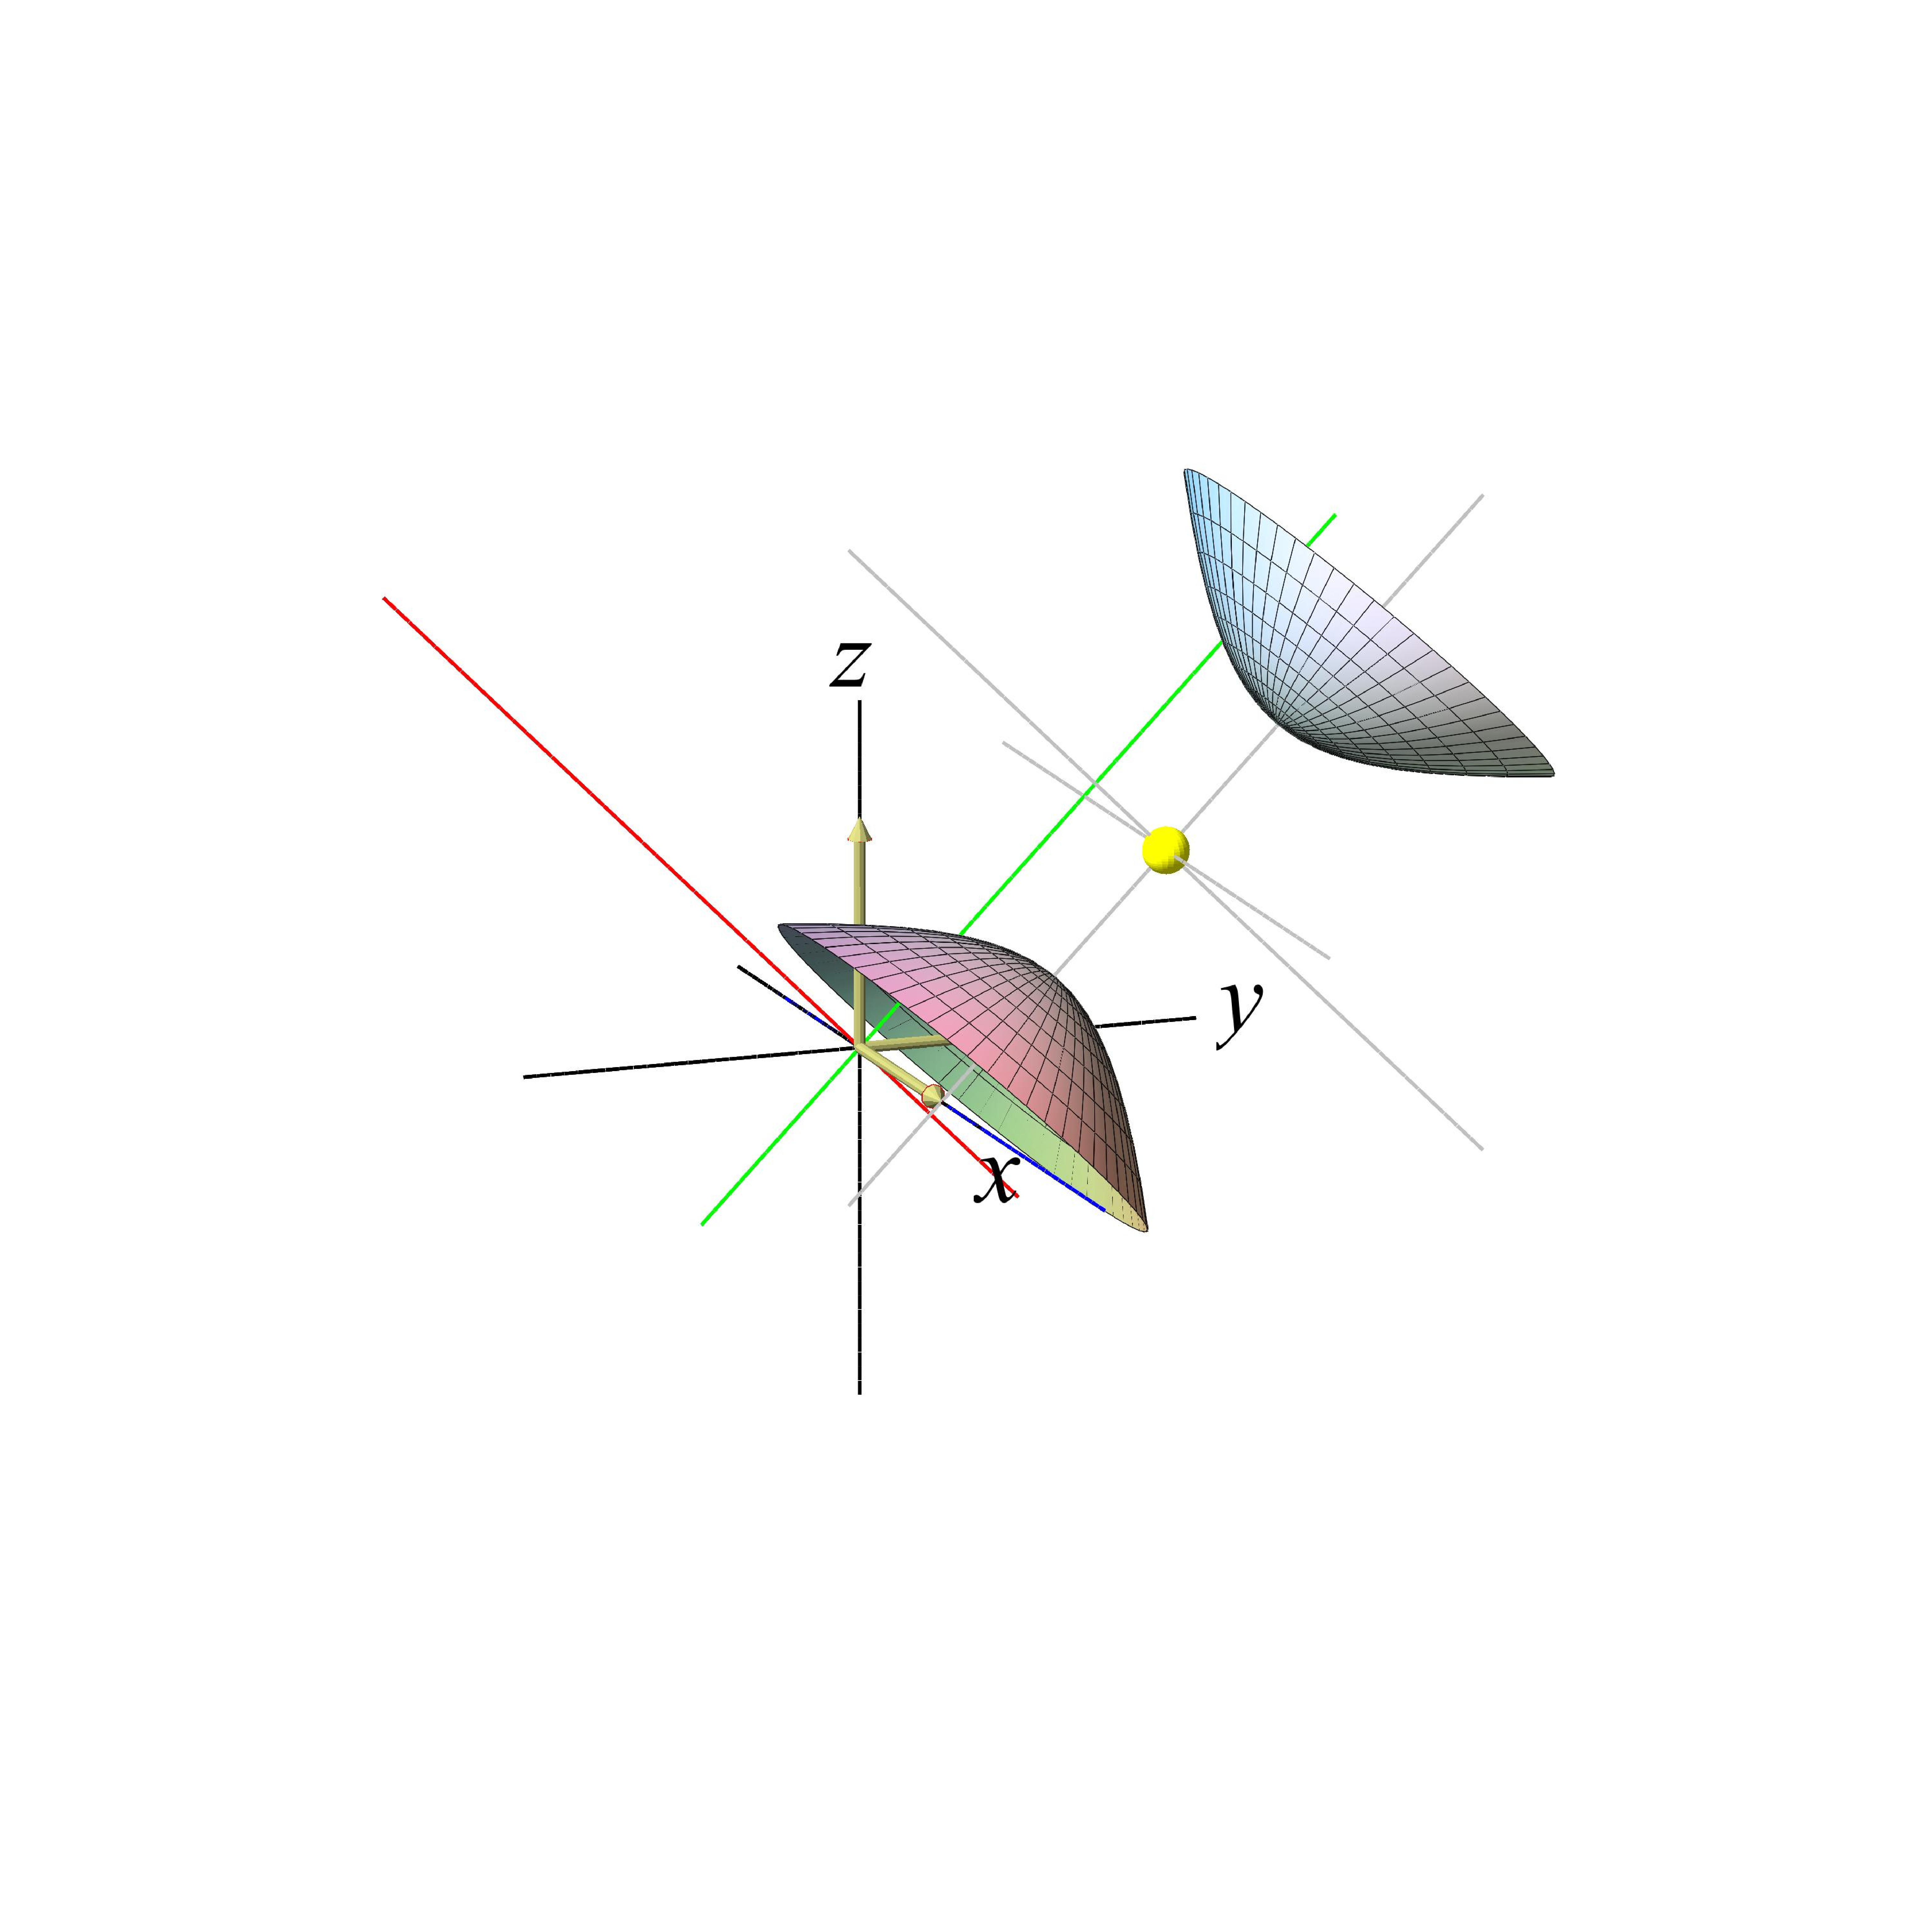
\includegraphics[height=80mm]{FIGS/plotHypTo3D01Kvad.pdf}}
\begin{center}
\caption{En hyperboloide med to net er niveaufladen $\mathcal{K}_{0}(f)$ for den funktion, der analyseres i eksempel \ref{exampHypTo3D01}.} \label{figHypTo3D01Kvad}
\end{center}
\end{figure}















%%%%%%%%%%%%%%%%%%%%%%%%%%%%%%%%%%%%%%%%%%%%%%%%%%%%%%%%%%%%%
%%%%%%%%%%%%%%%%%%%%%%%%%%%%%%%%%%%%%%%%%%%%%%%%%%%%%%%%%%%%%
%%%%%%%%%%%%%%%%%%%%%%%%%%%%%%%%%%%%%%%%%%%%%%%%%%%%%%%%%%%%%


\section{Navnetabel for andengradspolynomiers niveauflader} \label{secNavnetabel}

De maksimalt reducerede udtryk for andengradspolynomiers niveauflader præsenteres her under antagelse af at eventuelt centrum (eller såkaldt toppunkt) optræder i $\vekind{v}{\mathbf{C}} = (0,0,0)$. For en given konkret niveauflade kan navnet aflæses fra tabellen; beliggenheden angives med koordinaterne for det fundne centrum $\mathbf{C}$ for niveaufladen;  orienteringen angives ved den fundne substitutionsmatrix $\mathbf{Q}$ og størrelsen af niveaufladen angives ved de enkelte halvakser $a$, $b$, og  $c$, eller $p$ og $k$ i de enkelte tilfælde for så vidt de optræder i den reducerede ligning for niveaufladen.

\begin{equation*} \label{eqAndenGrad3D}
\begin{array}{|l|c|c|c|}
  \hline
  % after \\: \hline or \cline{col1-col2} \cline{col3-col4} ...
 \textrm{Ligning} & \textrm{Navn} & \textrm{Punktet $(0,0,0)$} & \textrm{Eksempel} \\ \hline \hline
  \frac{\widetilde{x}^{2}}{a^{2}} +  \frac{\widetilde{y}^{2}}{b^{2}} +   \frac{\widetilde{z}^{2}}{c^{2}} =1  & \textrm{ellipsoide} & \textrm{centrum} & \textrm{\ref{exampEllip3D01}} \\ \hline
  \frac{\widetilde{x}^{2}}{a^{2}} +  \frac{\widetilde{y}^{2}}{b^{2}} -  \frac{\widetilde{z}^{2}}{c^{2}} =1 & \textrm{hyperboloide med \'{e}t net} & \textrm{centrum} & \textrm{\ref{exampHypEt3D01}}\\ \hline
     \frac{\widetilde{x}^{2}}{a^{2}} - \frac{\widetilde{y}^{2}}{b^{2}} -   \frac{\widetilde{z}^{2}}{c^{2}} =1 & \textrm{hyperboloide med to net} & \textrm{centrum} & \textrm{\ref{exampHypTo3D01}}\\ \hline
  \frac{\widetilde{x}^{2}}{a^{2}} +  \frac{\widetilde{y}^{2}}{b^{2}} -   \frac{\widetilde{z}^{2}}{c^{2}} =0 & \textrm{keglesnitskegleflade} & \textrm{centrum} & \textrm{fig \ref{figGrafFlad}}\\ \hline
    \frac{\widetilde{x}^{2}}{a^{2}} +  \frac{\widetilde{y}^{2}}{b^{2}}  = \widetilde{z} & \textrm{elliptisk paraboloide} & \textrm{toppunkt}&  \textrm{fig \ref{figGrafFlad}}\\ \hline
   \frac{\widetilde{x}^{2}}{a^{2}} - \frac{\widetilde{y}^{2}}{b^{2}}  = \widetilde{z} & \textrm{hyperbolsk paraboloide} & \textrm{toppunkt}& \textrm{fig \ref{figGrafFlad}} \\ \hline
     \frac{\widetilde{x}^{2}}{a^{2}}= p\cdot \widetilde{z} & \textrm{parabolsk cylinderflade} & \textrm{toppunkt} & \textrm{fig \ref{figGrafFlad}} \\ \hline
 \frac{\widetilde{x}^{2}}{a^{2}} + \frac{\widetilde{y}^{2}}{b^{2}}  = 1 & \textrm{elliptisk cylinderflade} & \textrm{centrum} & \\ \hline
  \frac{\widetilde{x}^{2}}{a^{2}} - \frac{\widetilde{y}^{2}}{b^{2}}  = 1 & \textrm{hyperbolsk cylinderflade} & \textrm{centrum} & \\ \hline
\frac{\widetilde{x}^{2}}{a^{2}} +  \frac{\widetilde{y}^{2}}{b^{2}} +   \frac{\widetilde{z}^{2}}{c^{2}}  = 0 & \textrm{punktet $(0,0,0)$} & \textrm{''centrum''} & \\ \hline
 \frac{\widetilde{x}^{2}}{a^{2}} +  \frac{\widetilde{y}^{2}}{b^{2}}  = 0 & \textrm{$\widetilde{z}$-aksen} &  & \\ \hline
  \frac{\widetilde{x}^{2}}{a^{2}} -  \frac{\widetilde{y}^{2}}{b^{2}}  = 0 & \textrm{to planer gennem $\widetilde{z}$-aksen} &  & \\ \hline
\widetilde{x}^{2} =  k > 0  & \textrm{to planer parallelle med $(\widetilde{y},\widetilde{z})$-planen} &  & \\ \hline
 \widetilde{x}^{2} =  0  & \textrm{$(\widetilde{y},\widetilde{z})$-planen} &  & \\ \hline
 \hline
\end{array}
\end{equation*}





\begin{figure}[ht]
\centerline{  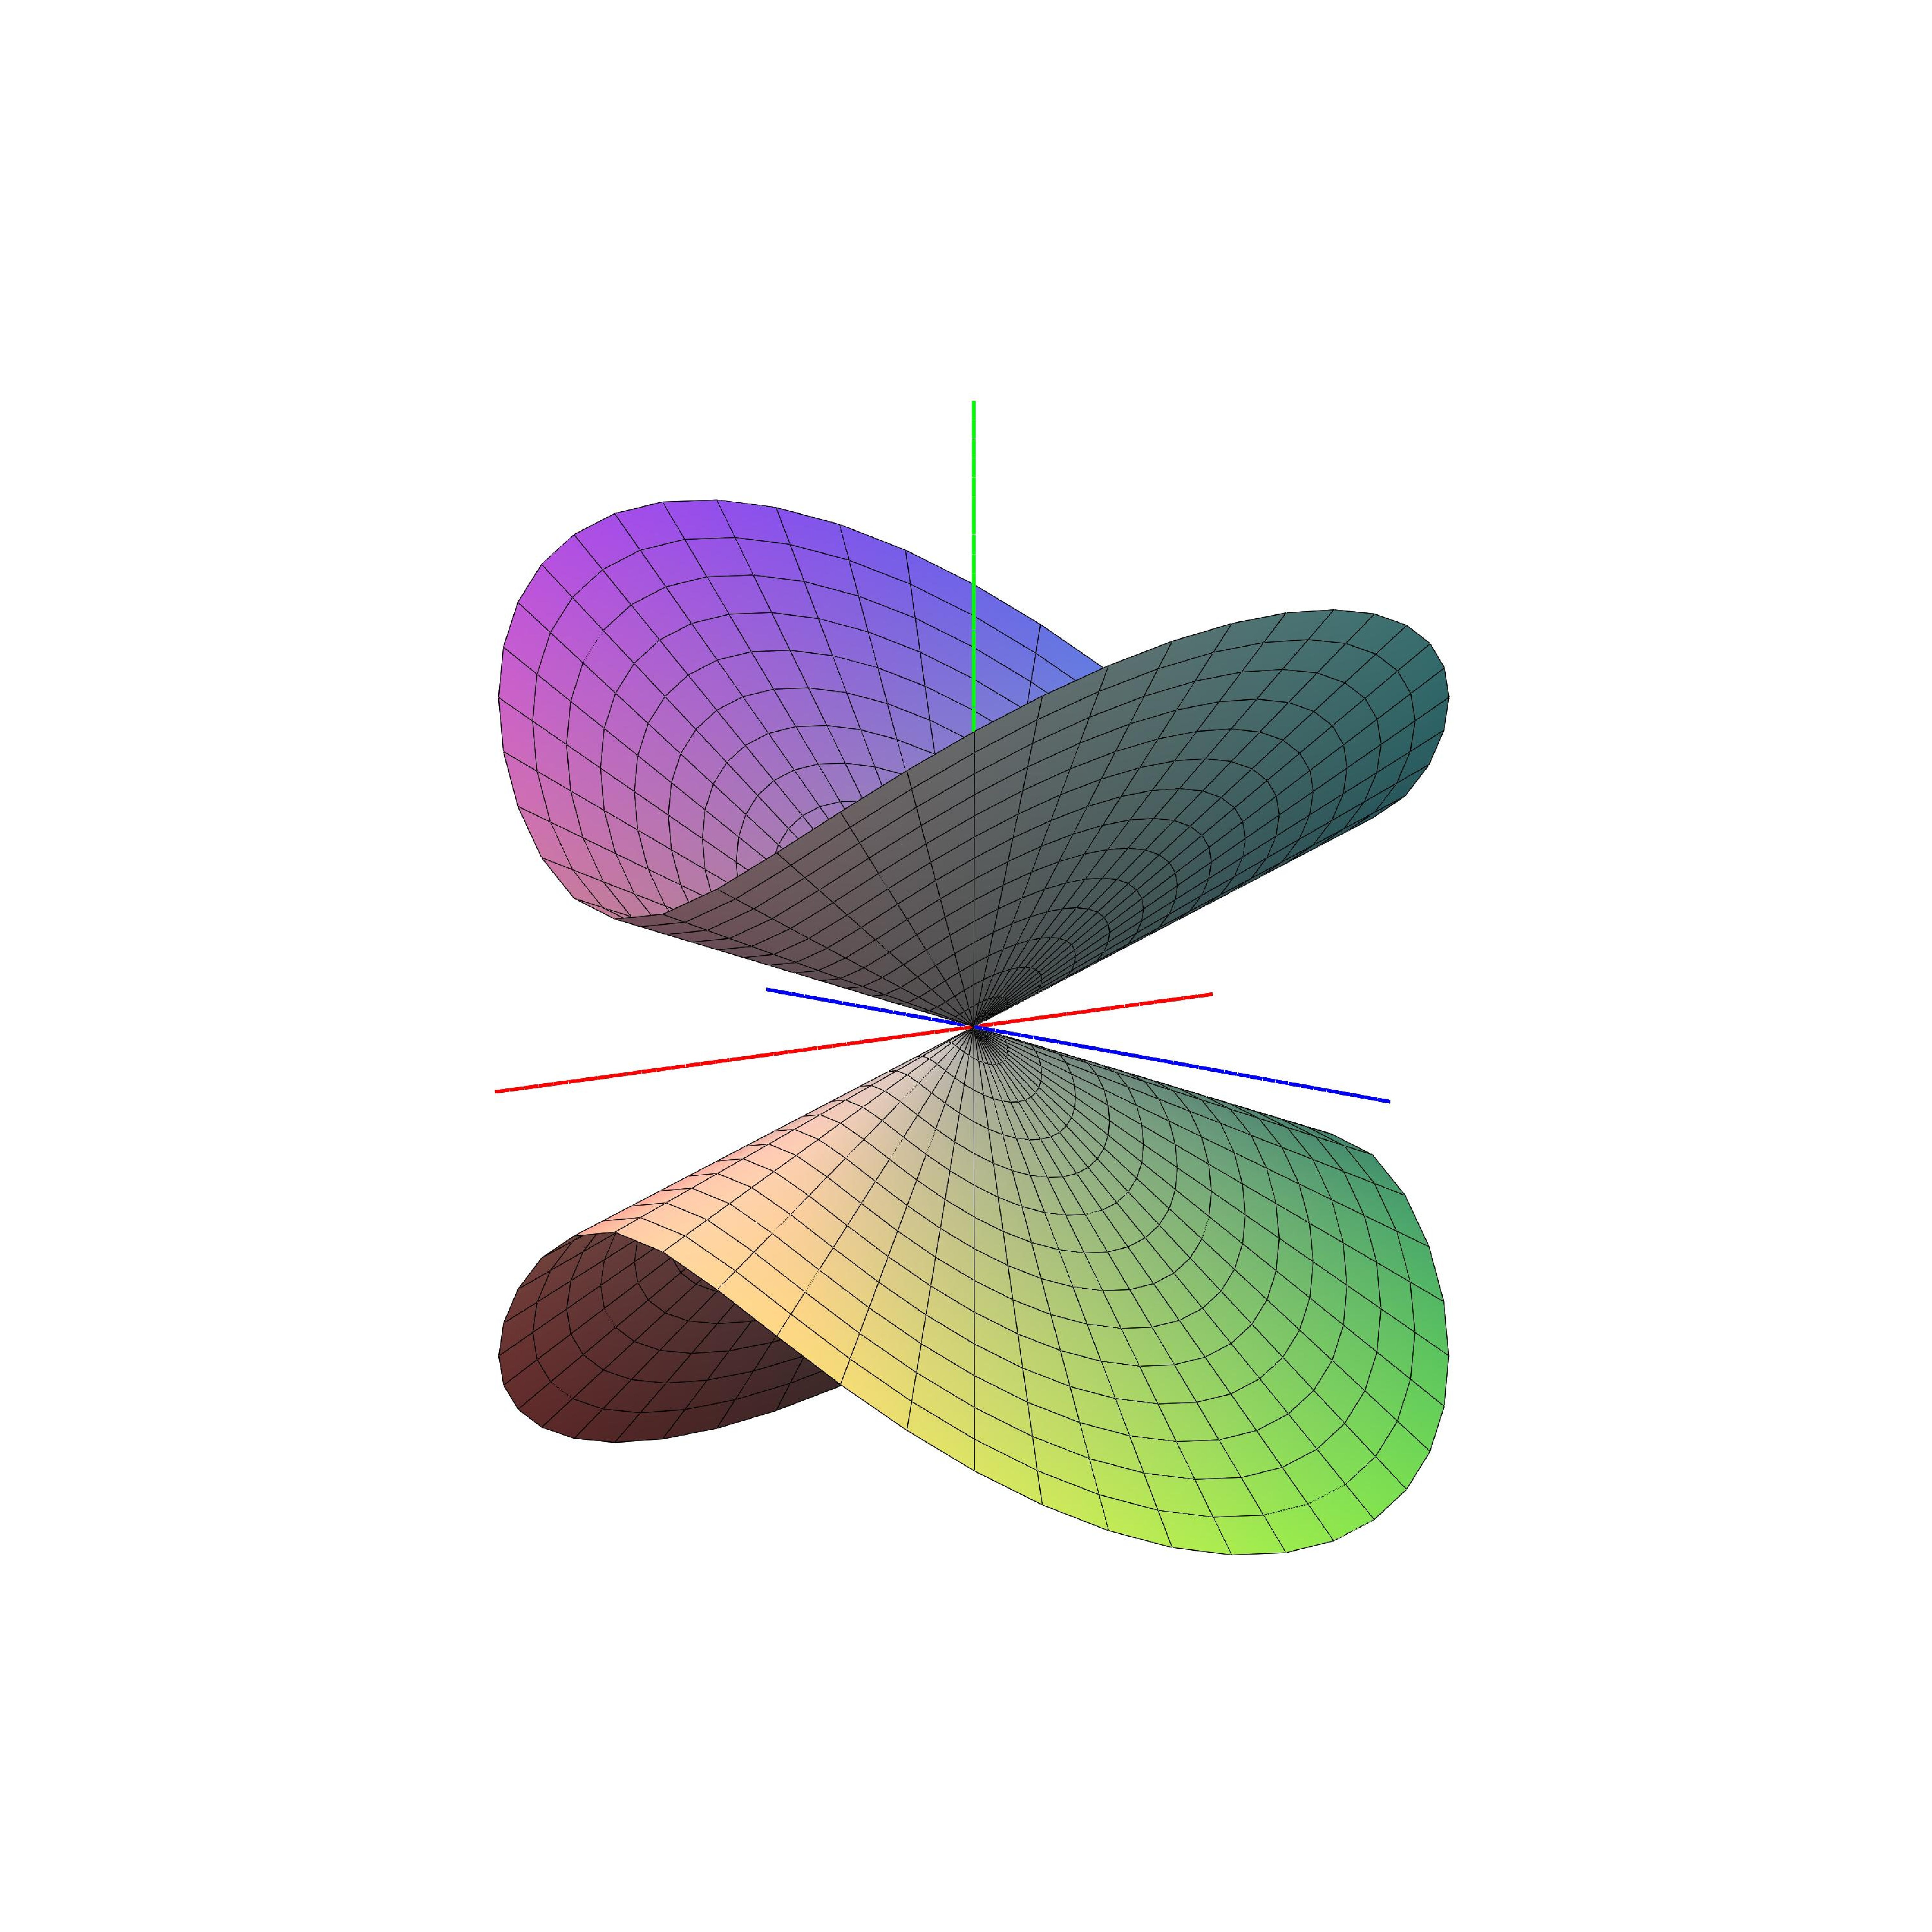
\includegraphics[height=45mm]{FIGS/plotKKegle.pdf} 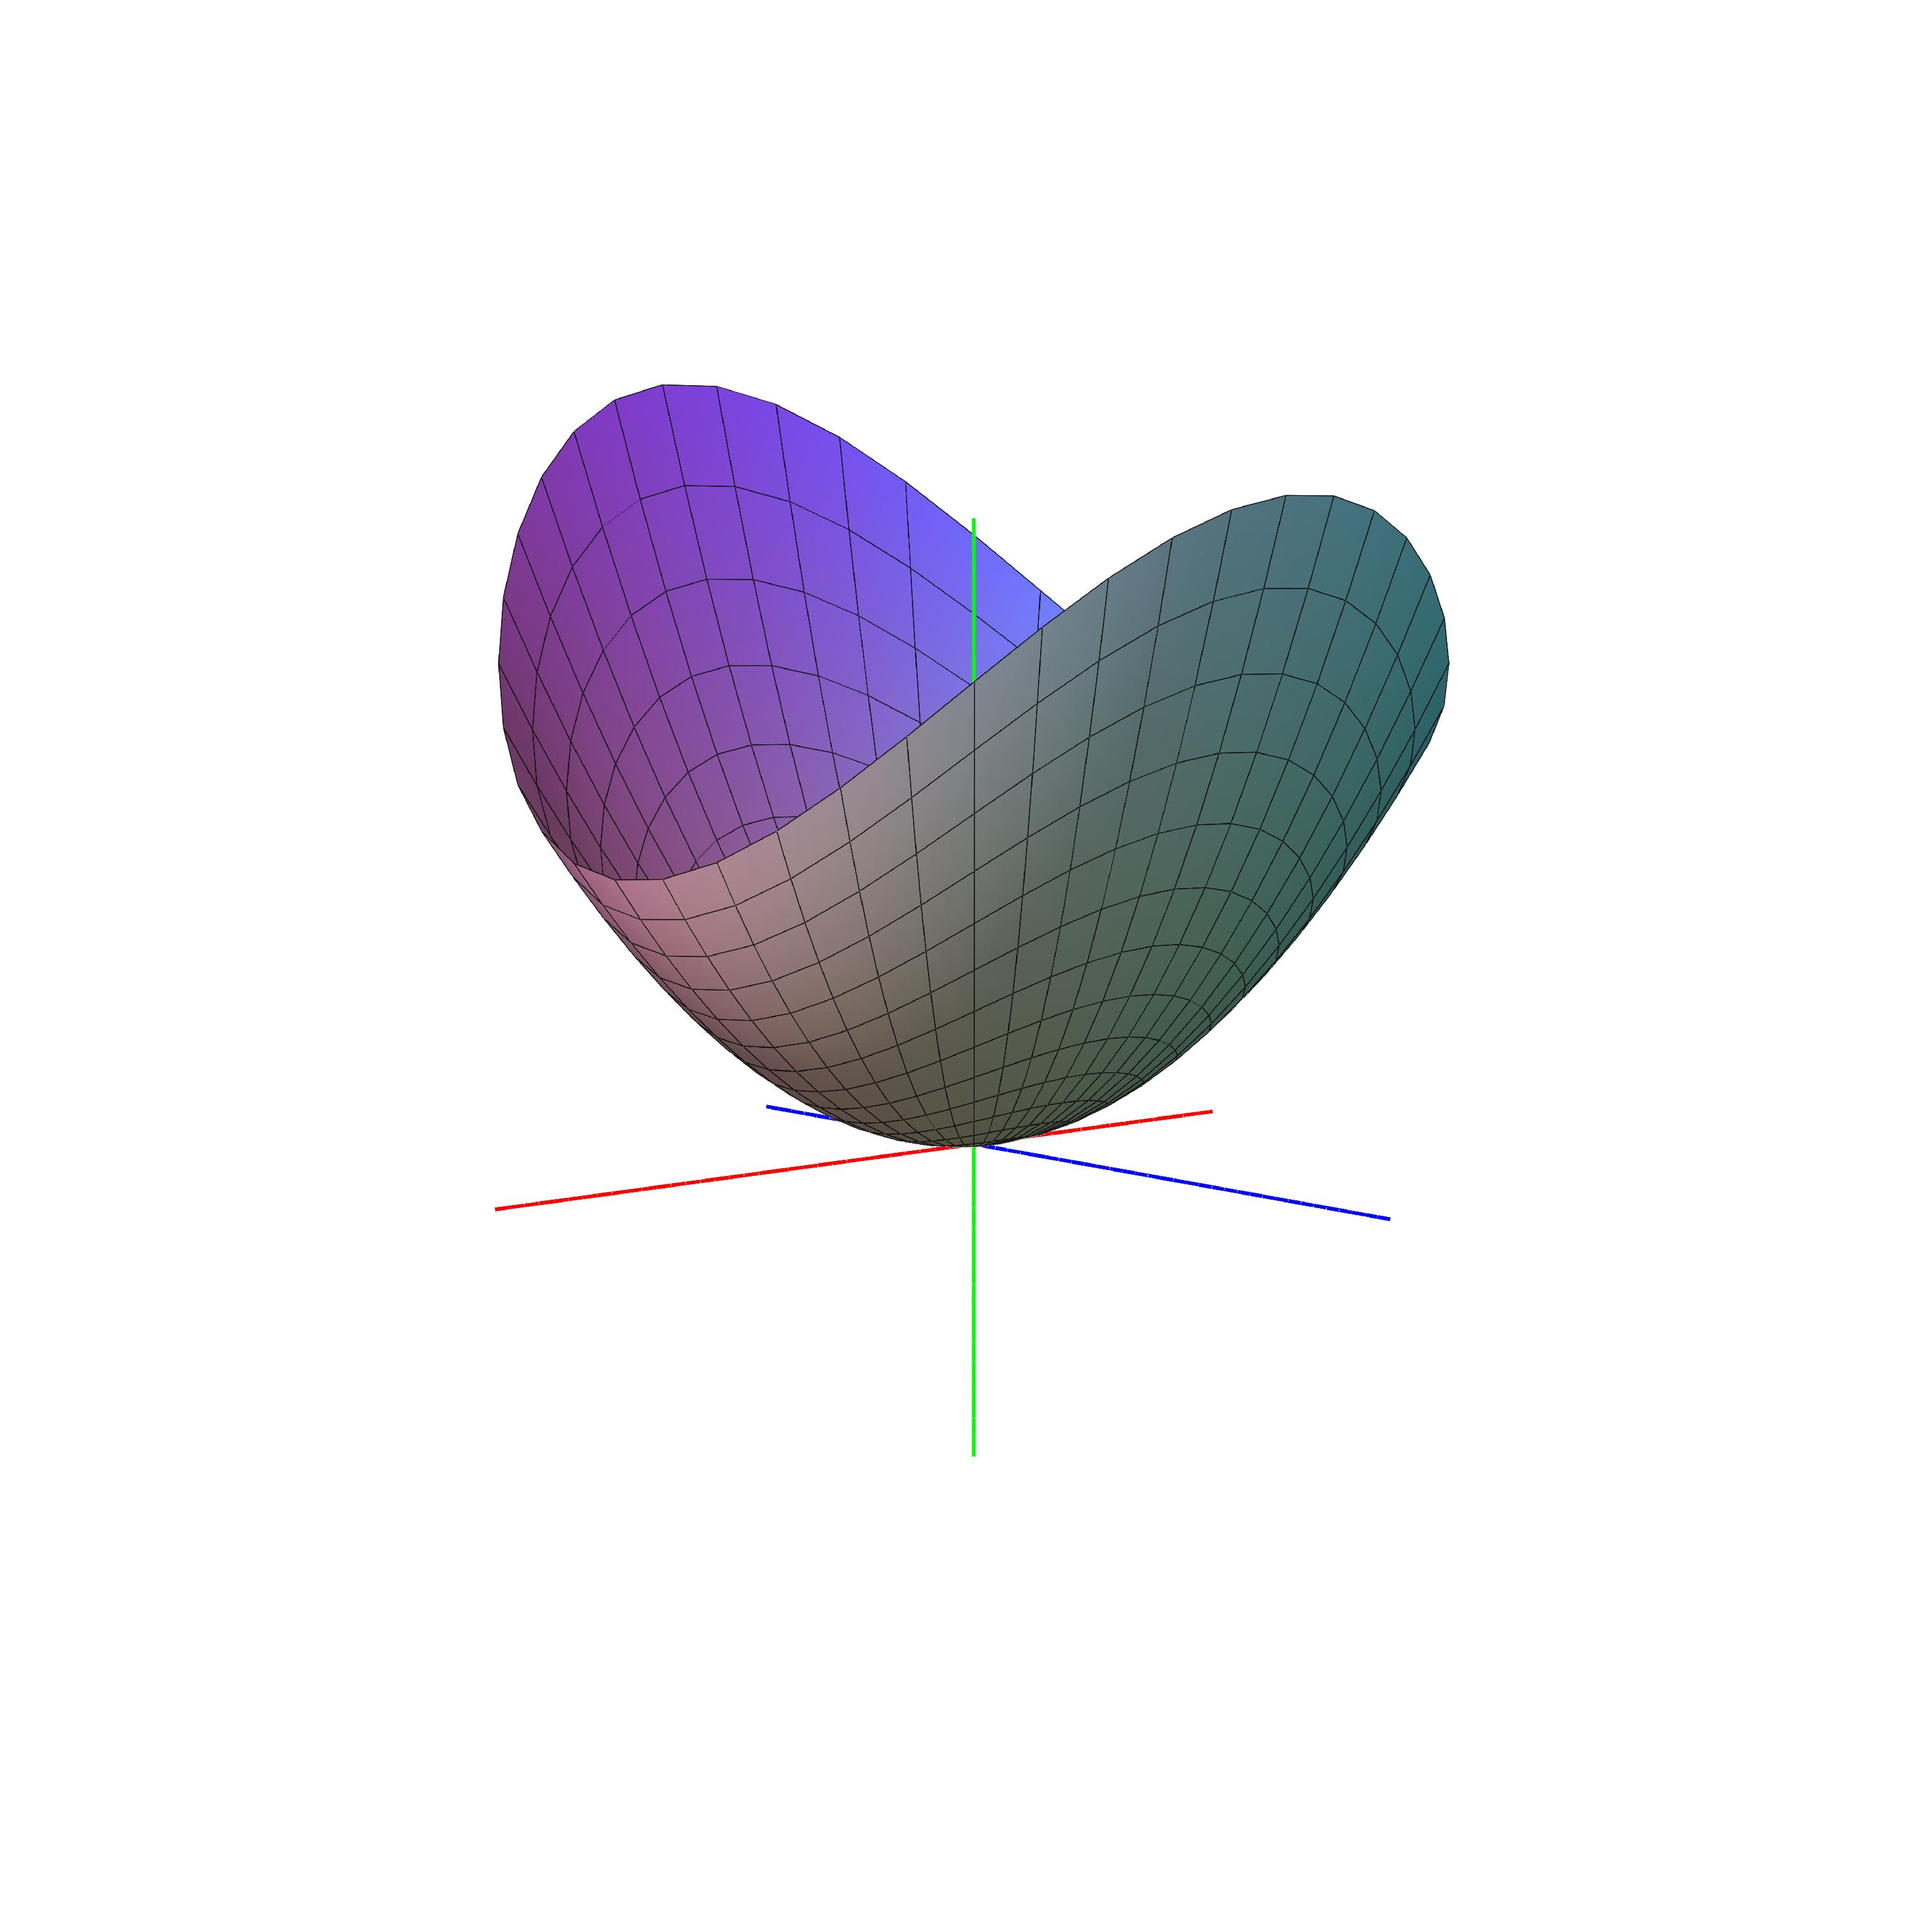
\includegraphics[height=45mm]{FIGS/plotEllipPar.pdf} 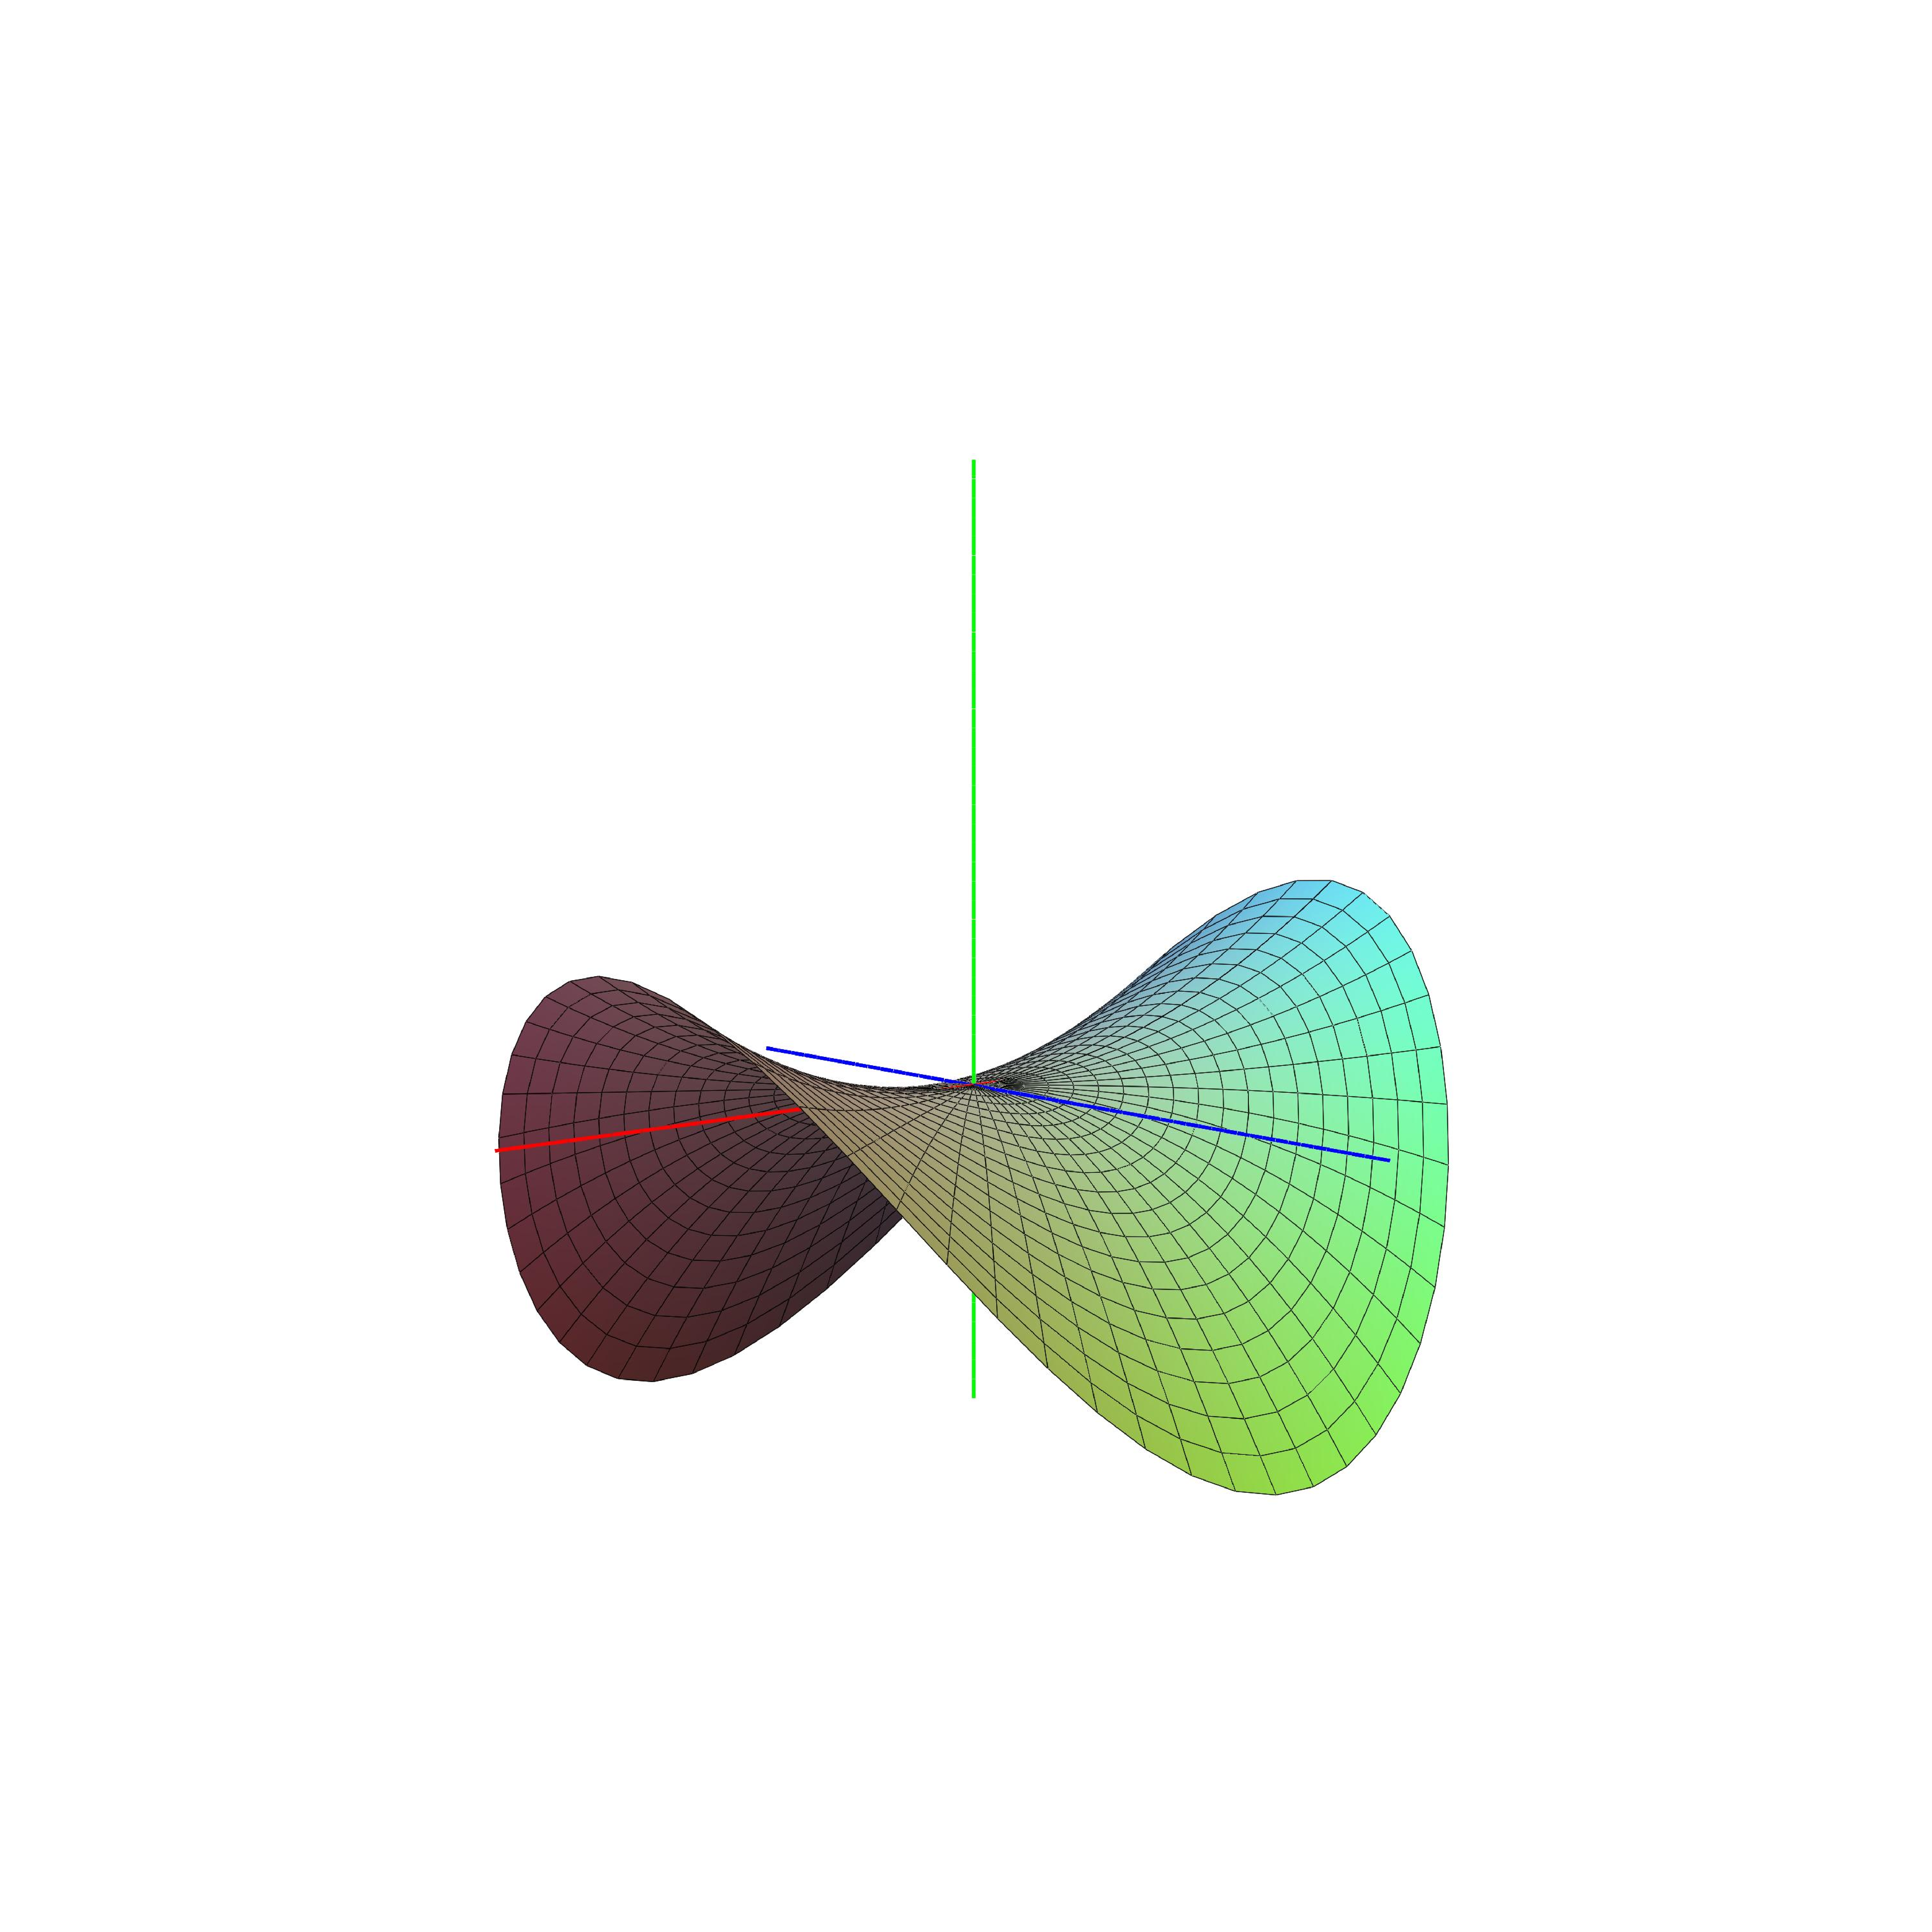
\includegraphics[height=45mm]{FIGS/plotHypPar.pdf} 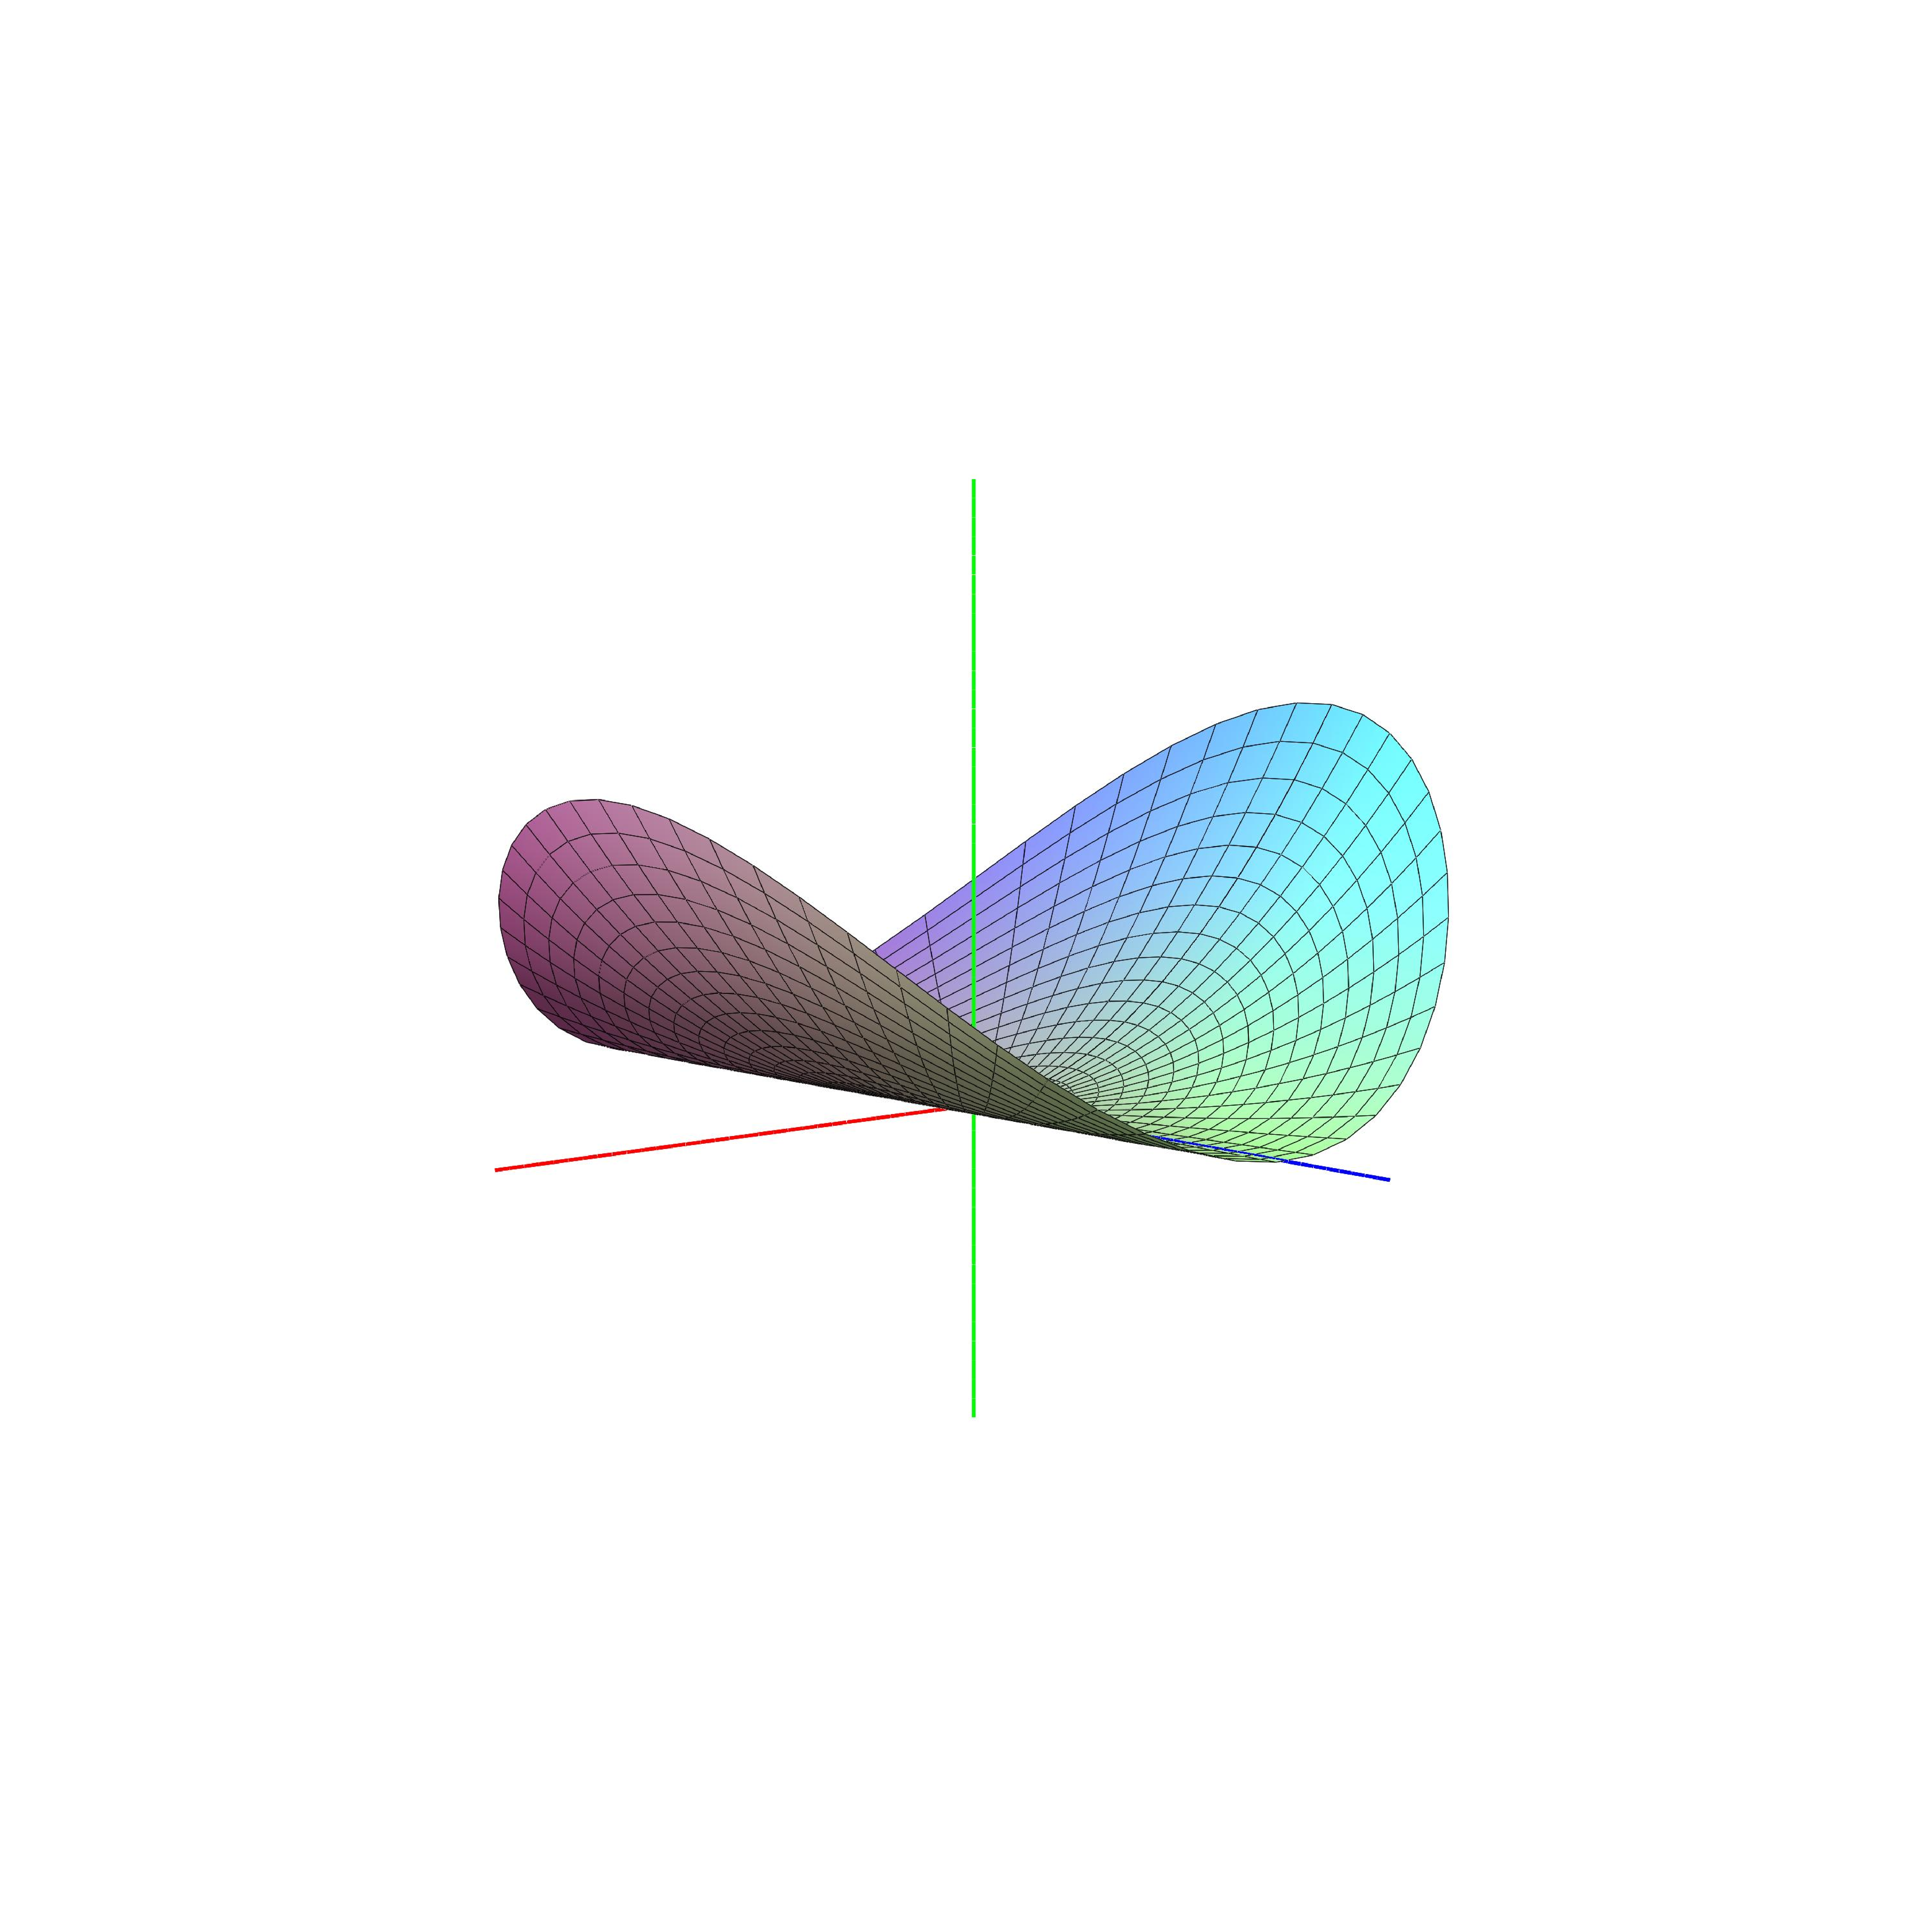
\includegraphics[height=45mm]{FIGS/plotParCyl.pdf} }
\begin{center}
\caption{En keglesnitskegleflade, en elliptisk paraboloide, en hyperbolsk paraboloide, og en parabolsk cylinderflade.} \label{figGrafFlad}
\end{center}
\end{figure}







\begin{exercise} \label{exercKomplet}
Vis, at listen i navnetabellen over niveauflader for andengradspolynomier i tre variable er komplet; dvs.  enhver totalt reduceret andengradsligning i tre variable (som indeholder mindst \'{e}n af de variable $\widetilde{x}$, $\widetilde{y}$, eller $\widetilde{z}$ med grad $2$) er at finde på listen.
\end{exercise}

\begin{exercise} \label{exercExtract2D}
Vis, at enhver totalt reduceret andengradsligning i to variable fremkommer af tabellen over totalt reducerede andengradsligninger i tre variable ved at sætte $\widetilde{z}=0$.
\end{exercise}

%%%%%%%%%%%%%%%%%%%%%%%%%%%%%%%%%%%%%%%%%%%%%%%%%%%%%%%%%%%%%
%%%%%%%%%%%%%%%%%%%%%%%%%%%%%%%%%%%%%%%%%%%%%%%%%%%%%%%%%%%%%
%%%%%%%%%%%%%%%%%%%%%%%%%%%%%%%%%%%%%%%%%%%%%%%%%%%%%%%%%%%%%


\section{Parametrisering af en ellipsoide}\label{secEllipsoideParam}

Vi vil her kort skitsere hvordan man kan \emph{parametrisere} en niveauflade for et andengrads\-polynomium i tre variable med henblik på at kunne plotte og undersøge dens øvrige geometriske egenskaber. Som eksempel vil vi benytte en ellipsoide
med givet (eller fundet) centrum $\mathbf{C}$, givne halvakser (aflæst fra diaognalmatricen  $\Lambda$), og givne orienterings-vektorer $\vekind{e}{\mathbf{v}_{1}}$, $\vekind{e}{\mathbf{v}_{2}}$, og  $\vekind{e}{\mathbf{v}_{3}}$ (fra den positive ortogonale substitutionsmatrix $\mathbf{Q}$) -- altså net\-op ud fra de data der bestemmes via reduktionsanalysen eksemplificeret ovenfor.\\

 Vi antager for eksemplets skyld, at der her er tale om en ellipsoide, således at $\mathbf{A} = \frac{1}{2}\cdot \mathbf{H}f(x,y, z)$ er positiv definit, dvs. alle tre egenværdier $\lambda_{1}$, $\lambda_{2}$, og $\lambda_{3}$ er positive for $\mathbf{A} = \frac{1}{2}\cdot \mathbf{H}f(x,y, z)$. Tilsvarende konstruktion kan gennemføres for enhver af  de andre niveauflader.\\

Vi antager, at ellipsoidens ligning i reduceret form er givet ved
\begin{equation}
\lambda_{1}\cdot(\widetilde{x}- \widetilde{x_{0}})^{2} + \lambda_{2}\cdot(\widetilde{y}- \widetilde{y_{0}})^{2} +\lambda_{3}\cdot(\widetilde{z}- \widetilde{z_{0}})^{2} = d^{2} \quad,
\end{equation}
hvor $d$ er en positiv konstant og hvor $\vekind{v}{\mathbf{C}} = (\widetilde{x_{0}}, \widetilde{y_{0}}, \widetilde{z_{0}})$ er koordinaterne for ellipsoidens centrum med hensyn til det nye koordinatsystem, således at centerkoordinaterne med hensyn til det gamle system er givet ved:
$\vekind{e}{\mathbf{C}} = \mathbf{Q}\cdot \vekind{v}{\mathbf{C}}$.
 Vi har altså følgende ingredienser til rådighed til konstruktionen af ellipsoiden:
\begin{equation}
\begin{aligned}
\vekind{e}{\mathbf{C}} &= (C_{1}, C_{2}, C_{3}) \\
a&= \frac{d}{\sqrt{\lambda_{1}}} \\
b&= \frac{d}{\sqrt{\lambda_{2}}} \\
c&= \frac{d}{\sqrt{\lambda_{3}}} \\
\mathbf{Q} &= \left[
               \begin{array}{ccc}
                 \vekind{e}{\mathbf{v}_{1}} &   \vekind{e}{\mathbf{v}_{2}} &   \vekind{e}{\mathbf{v}_{3}}\\
               \end{array}
             \right] \quad .
\end{aligned}
\end{equation}

Vi vil udelukkende betragte koordinater, der refererer til den sædvanlige basis e i $(\mathbb{R}^{n}, \bm{\cdot})$.

En kugleflade $\mathcal{S}_{1}$ med radius $1$ og centrum i $(0,0,0)$ kan  beskrives som mængden af de punkter $(x,y,z)$, der har afstanden $1$ til $(0,0,0)$:
\begin{equation} \label{eqSph}
\begin{aligned}
\rho_{(0,0,0)}(x,y,z) &= 1 \quad , \quad \textrm{som er ækvivalent med} \\
\quad \sqrt{x^{2} + y^{2} + z^{2}} &= 1 \quad , \quad \textrm{eller} \\
x^{2} + y^{2} + z^{2} &= 1 \quad.
\end{aligned}
\end{equation}

Kuglefladen kan også præsenteres ved hjælp af {\emph{geografiske koordinater}} $u$ og $v$, hvor $u \in [0, \pi]$ og $v\in [-\pi, \pi]$:
\begin{equation}
\mathcal{S} \quad : \quad (x,y,z) = \mathbf{r}(u,v) = (\sin(u)\cdot \cos(v), \sin(u)\cdot \sin(v), \cos(u) ) \quad.
\end{equation}
Når $u$ og $v$ gennemløber deres respektive intervaller $u \in [0, \pi]$ og $v\in [-\pi, \pi]$ så får vi punkter $(x,y,z) = \mathbf{r}(u,v)$ på kuglefladen -- og alle punkterne rammes.
Lad os se på den første af de to påstande, altså at alle punkterne $\mathbf{r}(u,v)$ ligger på kuglefladen. Indsæt $x=\sin(u)\cdot \cos(v)$, $y= \sin(u)\cdot \sin(v)$, og $z= \cos(u)$ i kuglens ligning \ref{eqSph}:
\begin{equation}
\begin{aligned}
x^{2} + y^{2} + z^{2} &= \sin^{2}(u)\cdot \cos^{2}(v) + \sin^{2}(u)\cdot \sin^{2}(v) + \cos^{2}(u) \\
&= \sin^{2}(u)\cdot \left(\sin^{2}(u) +  \cos^{2}(u)\right) + \cos^{2}(u) \\
&= \sin^{2}(u) + \cos^{2}(u) = 1 \quad,
\end{aligned}
\end{equation}
så alle punkterne der fremstilles på formen $\mathbf{r}(u,v)$ ligger på kuglefladen.

\begin{exercise} \label{exercSphCheck}
Vis, at den anden påstand om $\mathbf{r}(u,v)$ også er rigtig, altså at alle punkter på kuglefladen 'rammes' af $\mathbf{r}(u,v)$ når $u$ og $v$ gennemløber intervallerne $u \in [0, \pi]$ og $v \in [-\pi, \pi]$. Findes der punkter på kuglefladen som rammes mere end \'{e}n gang? Beskriv i så fald den punktmængde og hvor 'mange gange' de punkter rammes.
\end{exercise}

Vi skalerer kuglefladen med de tre egenværdier i hver koordinatakseretning og får dermed en fremstilling af en ellipsoide med de korrekte, ønskede, halvakser:
\begin{equation}
{\mathbf{r}_{1}}(u,v) = (\frac{d}{\sqrt{\lambda_{1}}}\cdot \sin(u)\cdot \cos(v), \frac{d}{\sqrt{\lambda_{2}}}\cdot \sin(u)\cdot \sin(v),  \frac{d}{\sqrt{\lambda_{3}}}\cdot \cos(u) )    \quad ,
\end{equation}
hvor $\quad  u \in [0, \pi] \, , \,  v\in [-\pi, \pi]$
således at ethvert punkt $x, y,z$ som rammes af afbildningen  ${\mathbf{r}}_{1}(u,v)$ nu tilfredsstiller:
\begin{equation}
\begin{aligned}
\lambda_{1}\cdot {x}^{2} + \lambda_{2}\cdot {y}^{2} + \lambda_{3}\cdot {z}^{2} &= d^{2} \\ \\
\left(\frac{{x}}{\frac{d}{\sqrt{\lambda_{1}}}}\right)^{2} + \left(\frac{{y}}{\frac{d}{\sqrt{\lambda_{2}}}}\right)^{2} + \left(\frac{{z}}{\frac{d}{\sqrt{\lambda_{3}}}}\right)^{2}  &= 1
\end{aligned}
\end{equation}
eller, hvis vi benytter halvaksebetegnelserne $a$, $b$, og $c$:
\begin{equation}
\left(\frac{{x}}{a}\right)^{2} + \left(\frac{{y}}{b}\right)^{2} + \left(\frac{{z}}{c}\right)^{2}  = 1 \quad ,
\end{equation}
som netop er ligningen for en standard ellipsoide med de ønskede halvakser men konstrueret i $(x,y,z)$-systemet. De punkter der fremstilles ved ${\mathbf{r}_{1}}(u,v)$ ligger alle på denne elipsoide.\\

Til sidst roterer vi ellipsoiden med rotationsmatricen $\mathbf{Q}$ og parallelforskyder til det korrekte ønskede centrum:

\begin{equation} \label{eqPamEllipGen}
{\mathbf{r}}_{2}(u,v) = \mathbf{Q}\cdot \mathbf{{r}}_{1}(u,v) + \mathbf{C} \quad.
\end{equation}
Alle de punkter, der har stedvektorer givet ved ${\mathbf{r}}_{2}(u,v)$ ligger nu på den ønskede ellipsoide og alle punkterne på ellipsoiden rammes når
$\quad  u \in [0, \pi] \, , \,  v\in [-\pi, \pi]$.

\begin{example}[Ellipsoide parametrisering] \label{exampEllipsoide}
En konkret ellipsoide er givet ved følgende data, som stammer fra en undersøgelse af andengradspolynomiet
\begin{equation}
 f(x,y, z) =  2\cdot x^{2} + 2\cdot y^{2} + 2\cdot z^{2} - 2\cdot x - 4\cdot y - 2 \cdot z - 2\cdot x \cdot z + 3 \quad :
\end{equation}
\begin{equation}
\begin{aligned}
\vekind{e}{\mathbf{C}} &= (1,1,1) \\
a&= \frac{1}{\sqrt{3}} \\
b&= \frac{1}{\sqrt{2}} \\
c&= 1 \\
\mathbf{Q} &= \left[
                \begin{array}{ccc}
                  -1/\sqrt{2} & 0 & -1/\sqrt{2} \\
                  0 & 1 & 0 \\
                  1/\sqrt{2} & 0 & -1/\sqrt{2} \\
                \end{array}
              \right] \quad .
\end{aligned}
\end{equation}

Vi vil konstruere en parameterfremstilling på formen ${\mathbf{r}}_{2}(u,v)$ som i (\ref{eqPamEllipGen}) for den givne ellipsoide.
Den skalerede kugleflade er givet ved:
\begin{equation}
{\mathbf{r}_{1}}(u,v) = \left(\frac{1}{\sqrt{3}}\cdot \sin(u) \cdot \cos(v) , \frac{1}{\sqrt{2}}\cdot \sin(u) \cdot \sin(v) , \cos(u) \right)
\end{equation}
og den $\mathbf{Q}$-roterede skalerede kugleflade parallelforskudt til punktet $(1,1,1)$ får derefter parameterfremstillingen:
\begin{equation}
\begin{aligned}
{\mathbf{r}}_{2}(u,v)  &= \\
&= (-\frac{1}{\sqrt{6}}\cdot \sin(u)\cdot \cos(v) - \frac{1}{\sqrt{2}}\cdot \cos(u) +1 \, , \\  \,
&\phantom{aaaa}\frac{1}{\sqrt{2}}\cdot \sin(u)\cdot \sin(v) + 1 \, , \\
&\phantom{aaaa}\frac{1}{\sqrt{6}}\cdot \sin(u)\cdot \cos(v) - \frac{1}{\sqrt{2}}\cdot \cos(u) + 1) \quad.
\end{aligned}
\end{equation}
Konstruktionen er antydet i figur \ref{figEllConstr}.
\end{example}

\begin{figure}[ht]
\centerline{  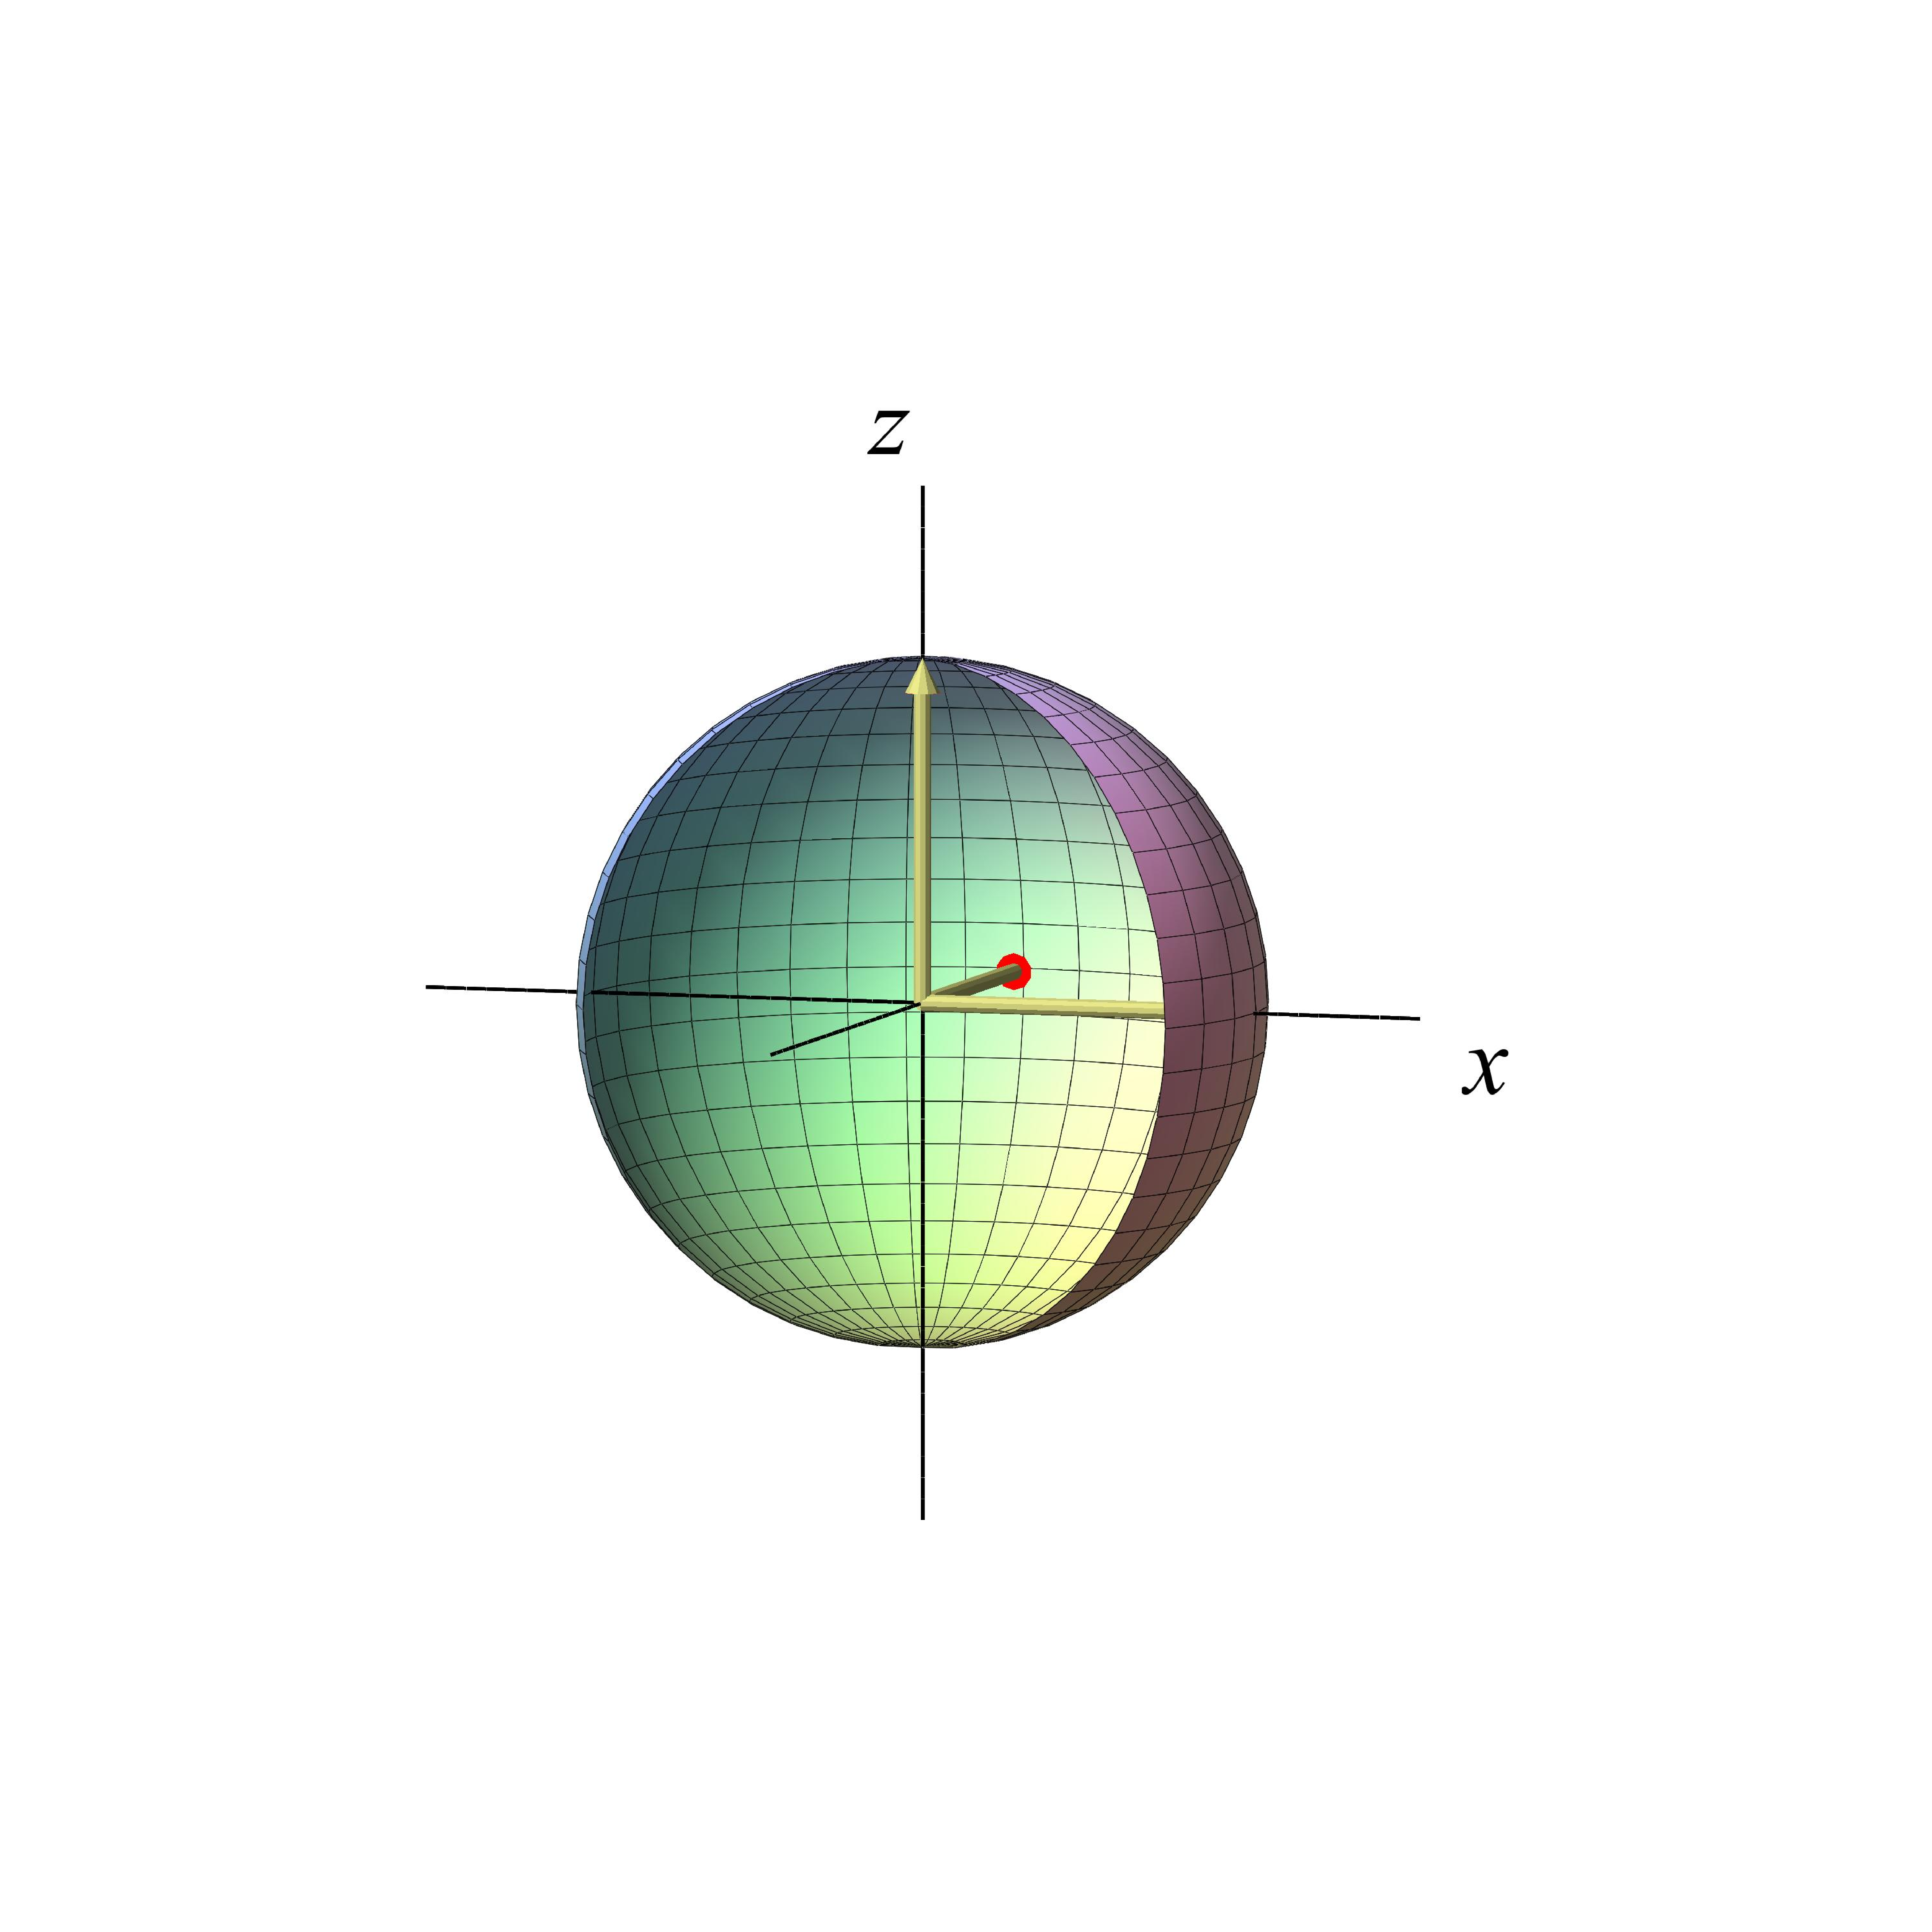
\includegraphics[height=40mm]{FIGS/plotEllConstr1.pdf} 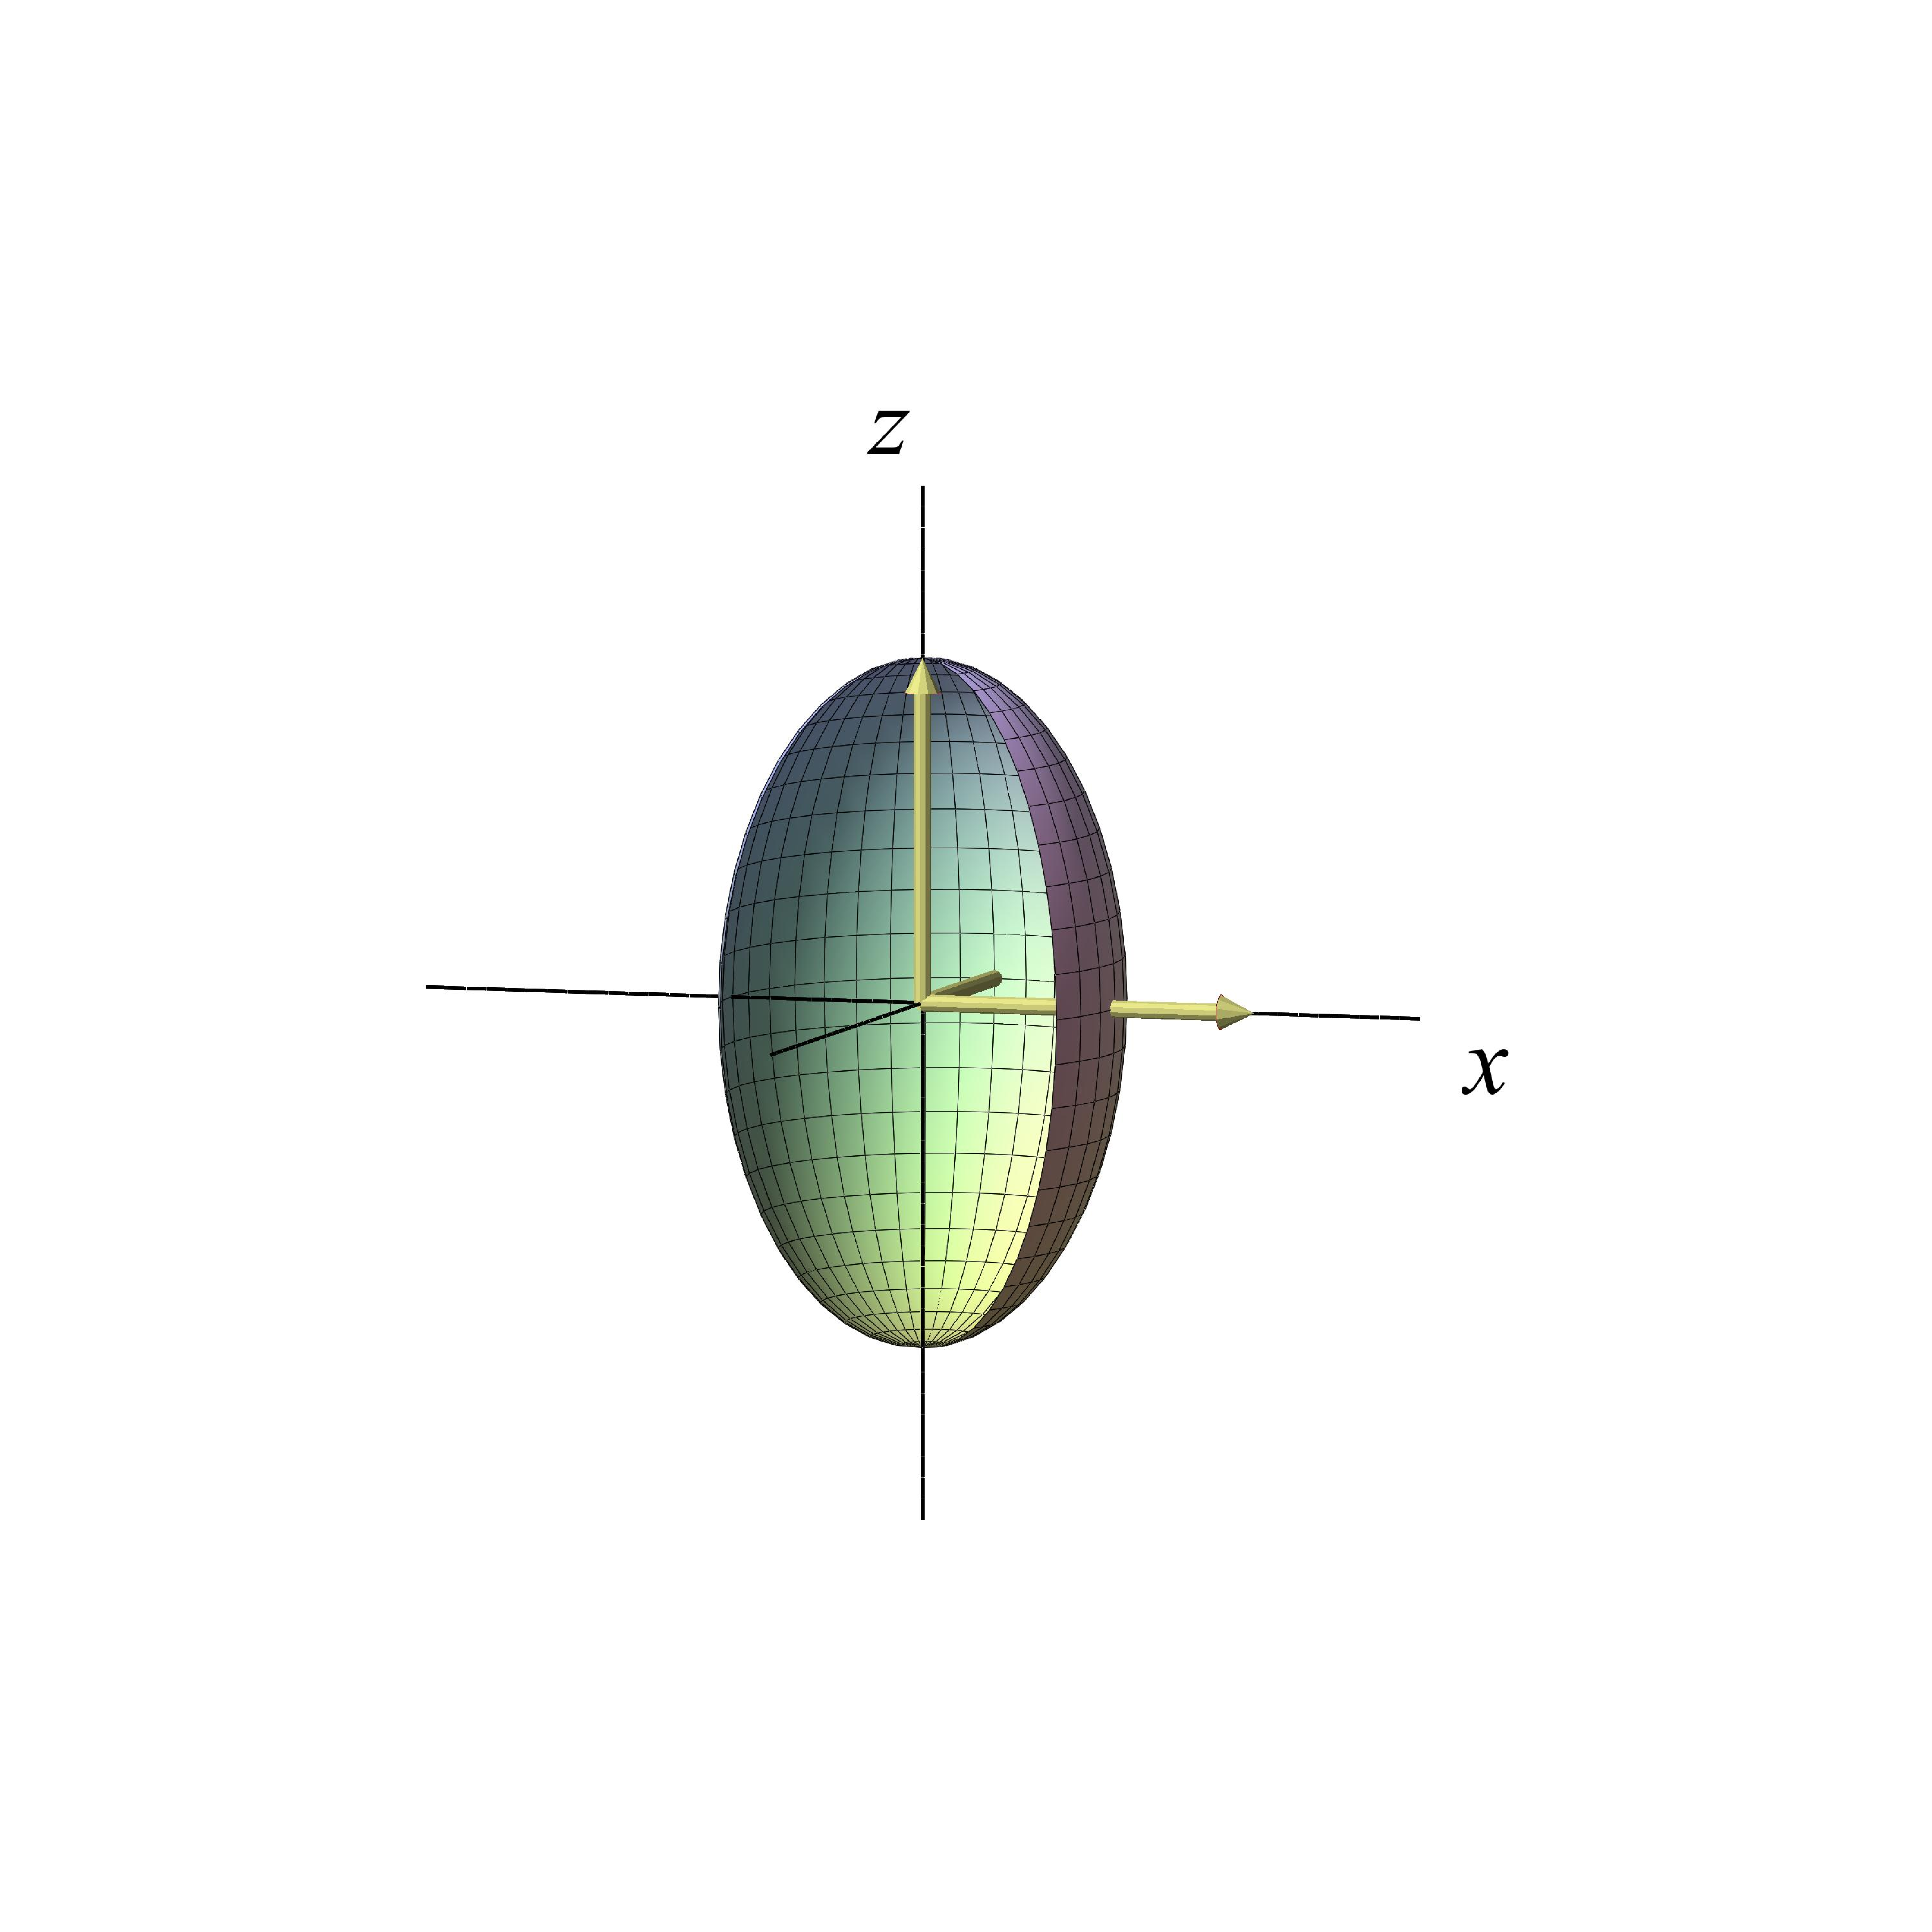
\includegraphics[height=40mm]{FIGS/plotEllConstr2.pdf} 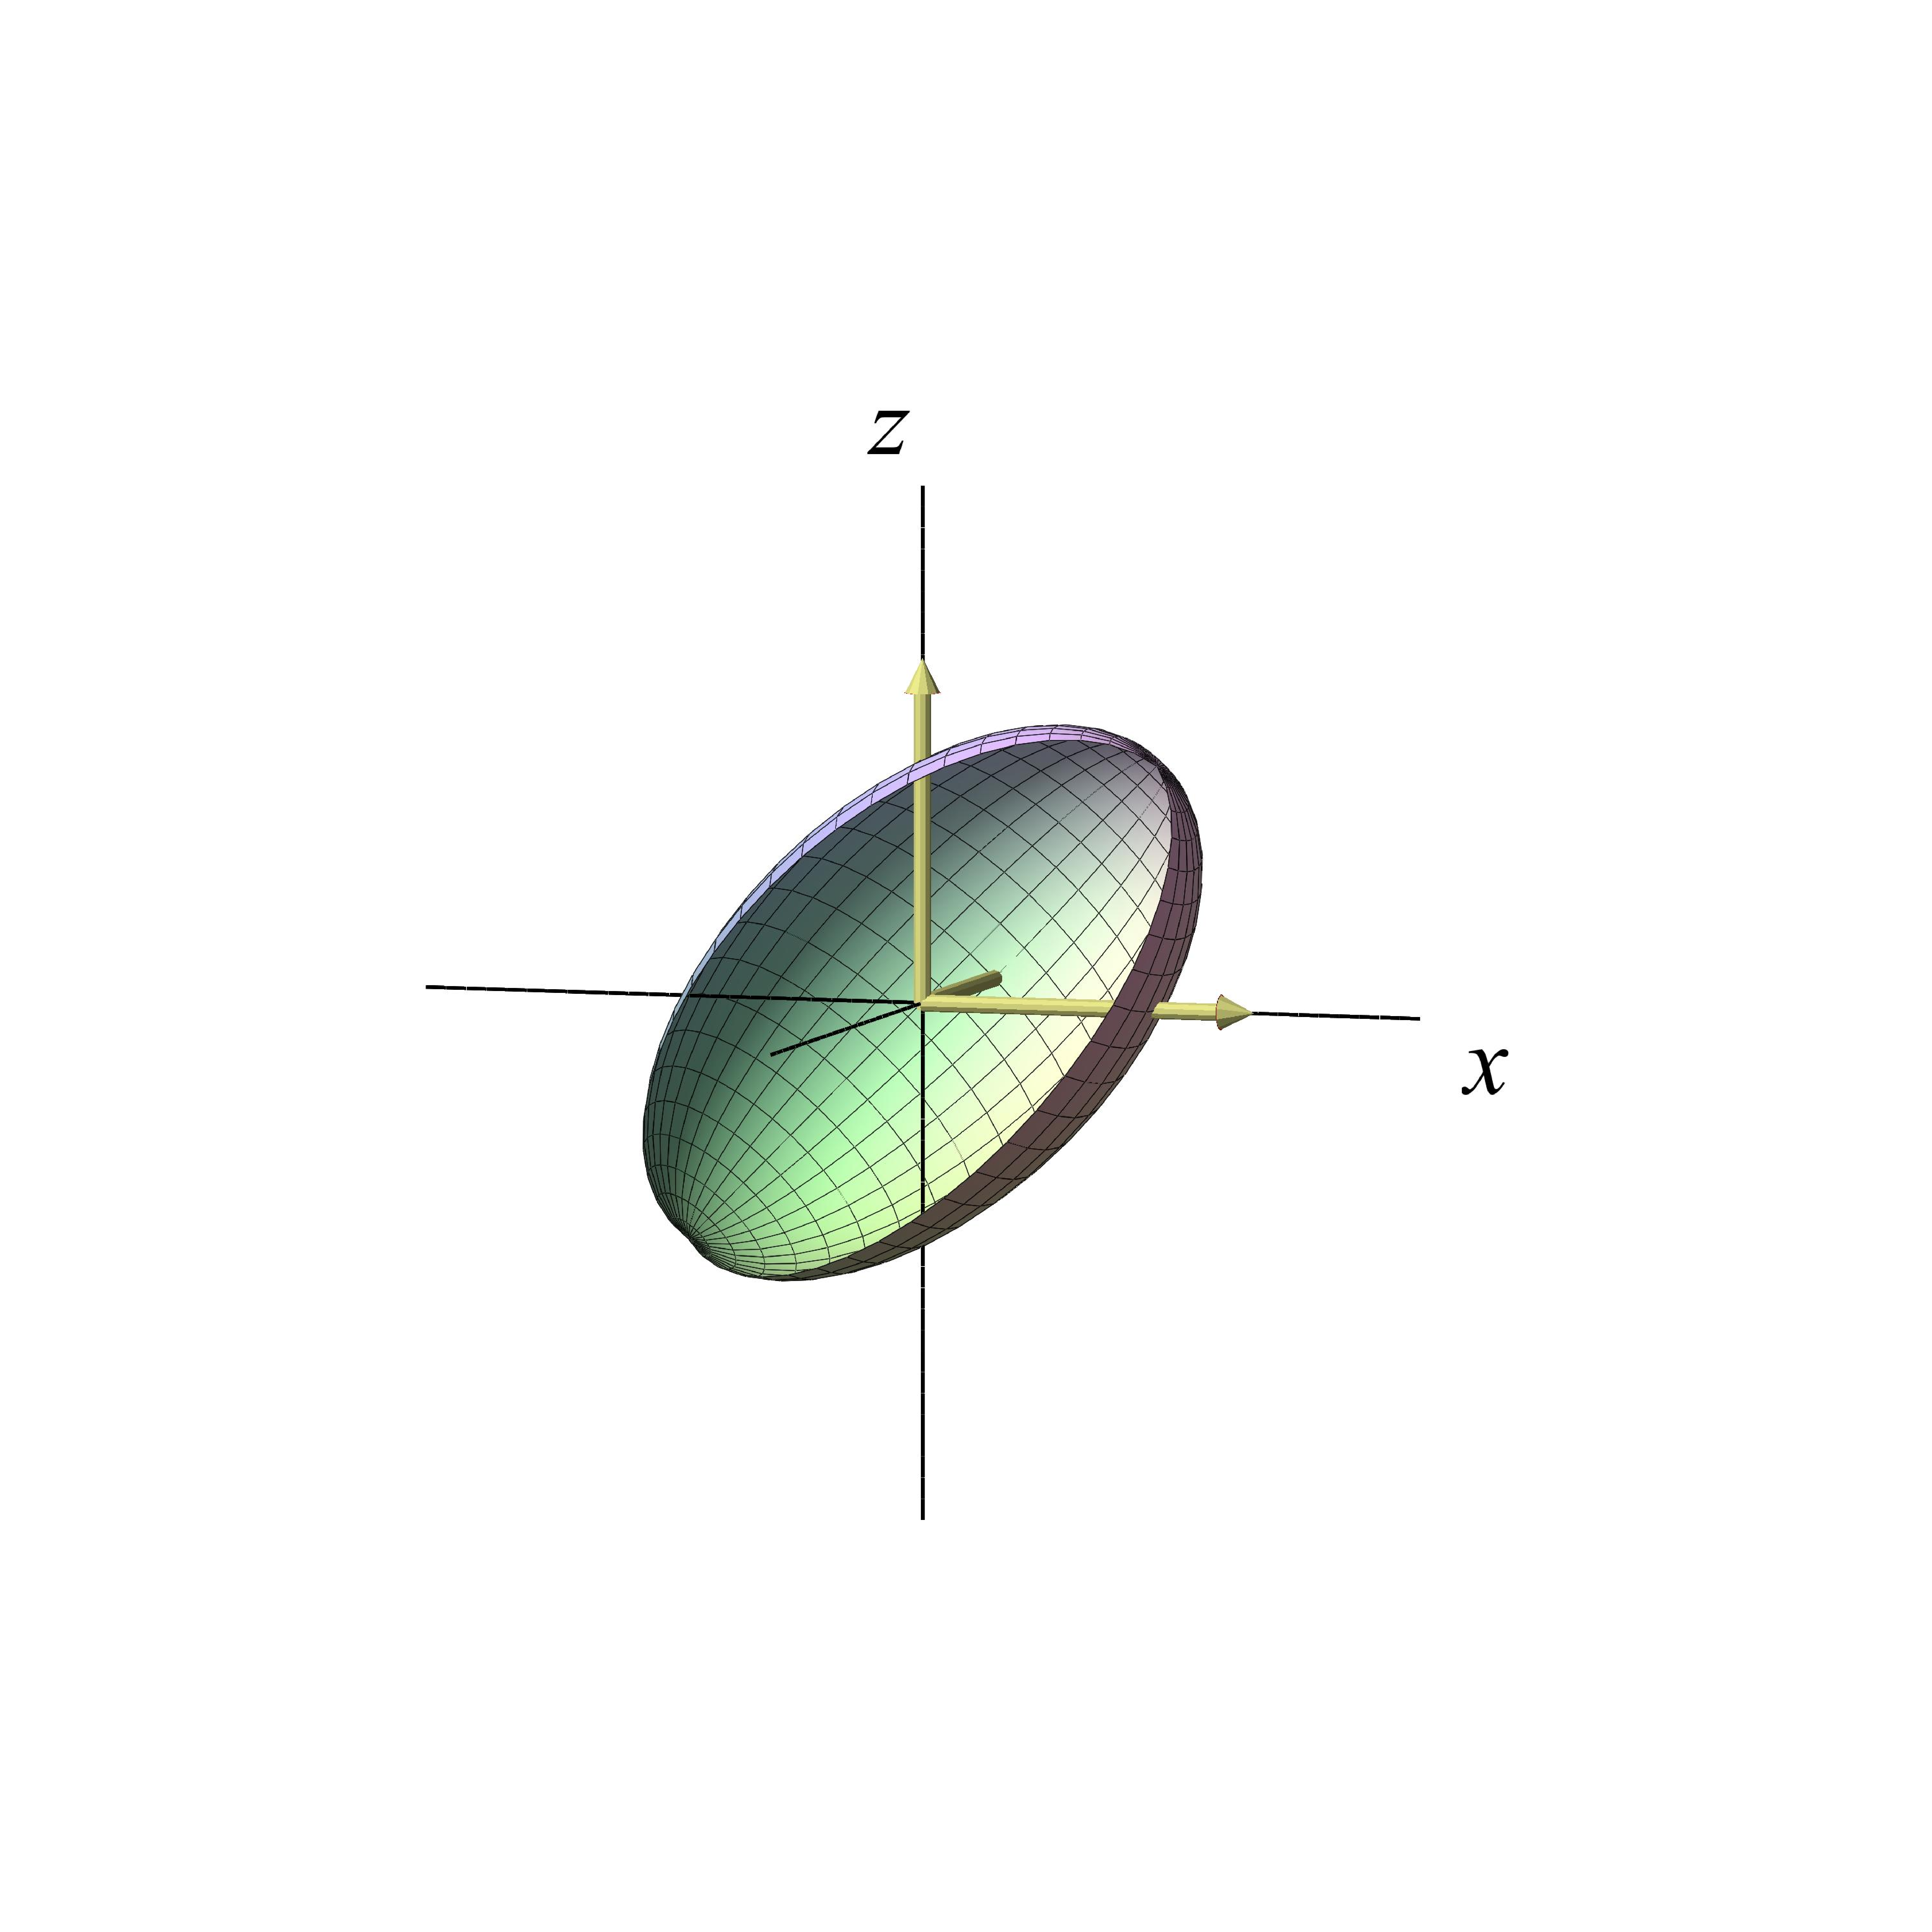
\includegraphics[height=40mm]{FIGS/plotEllConstr3.pdf}
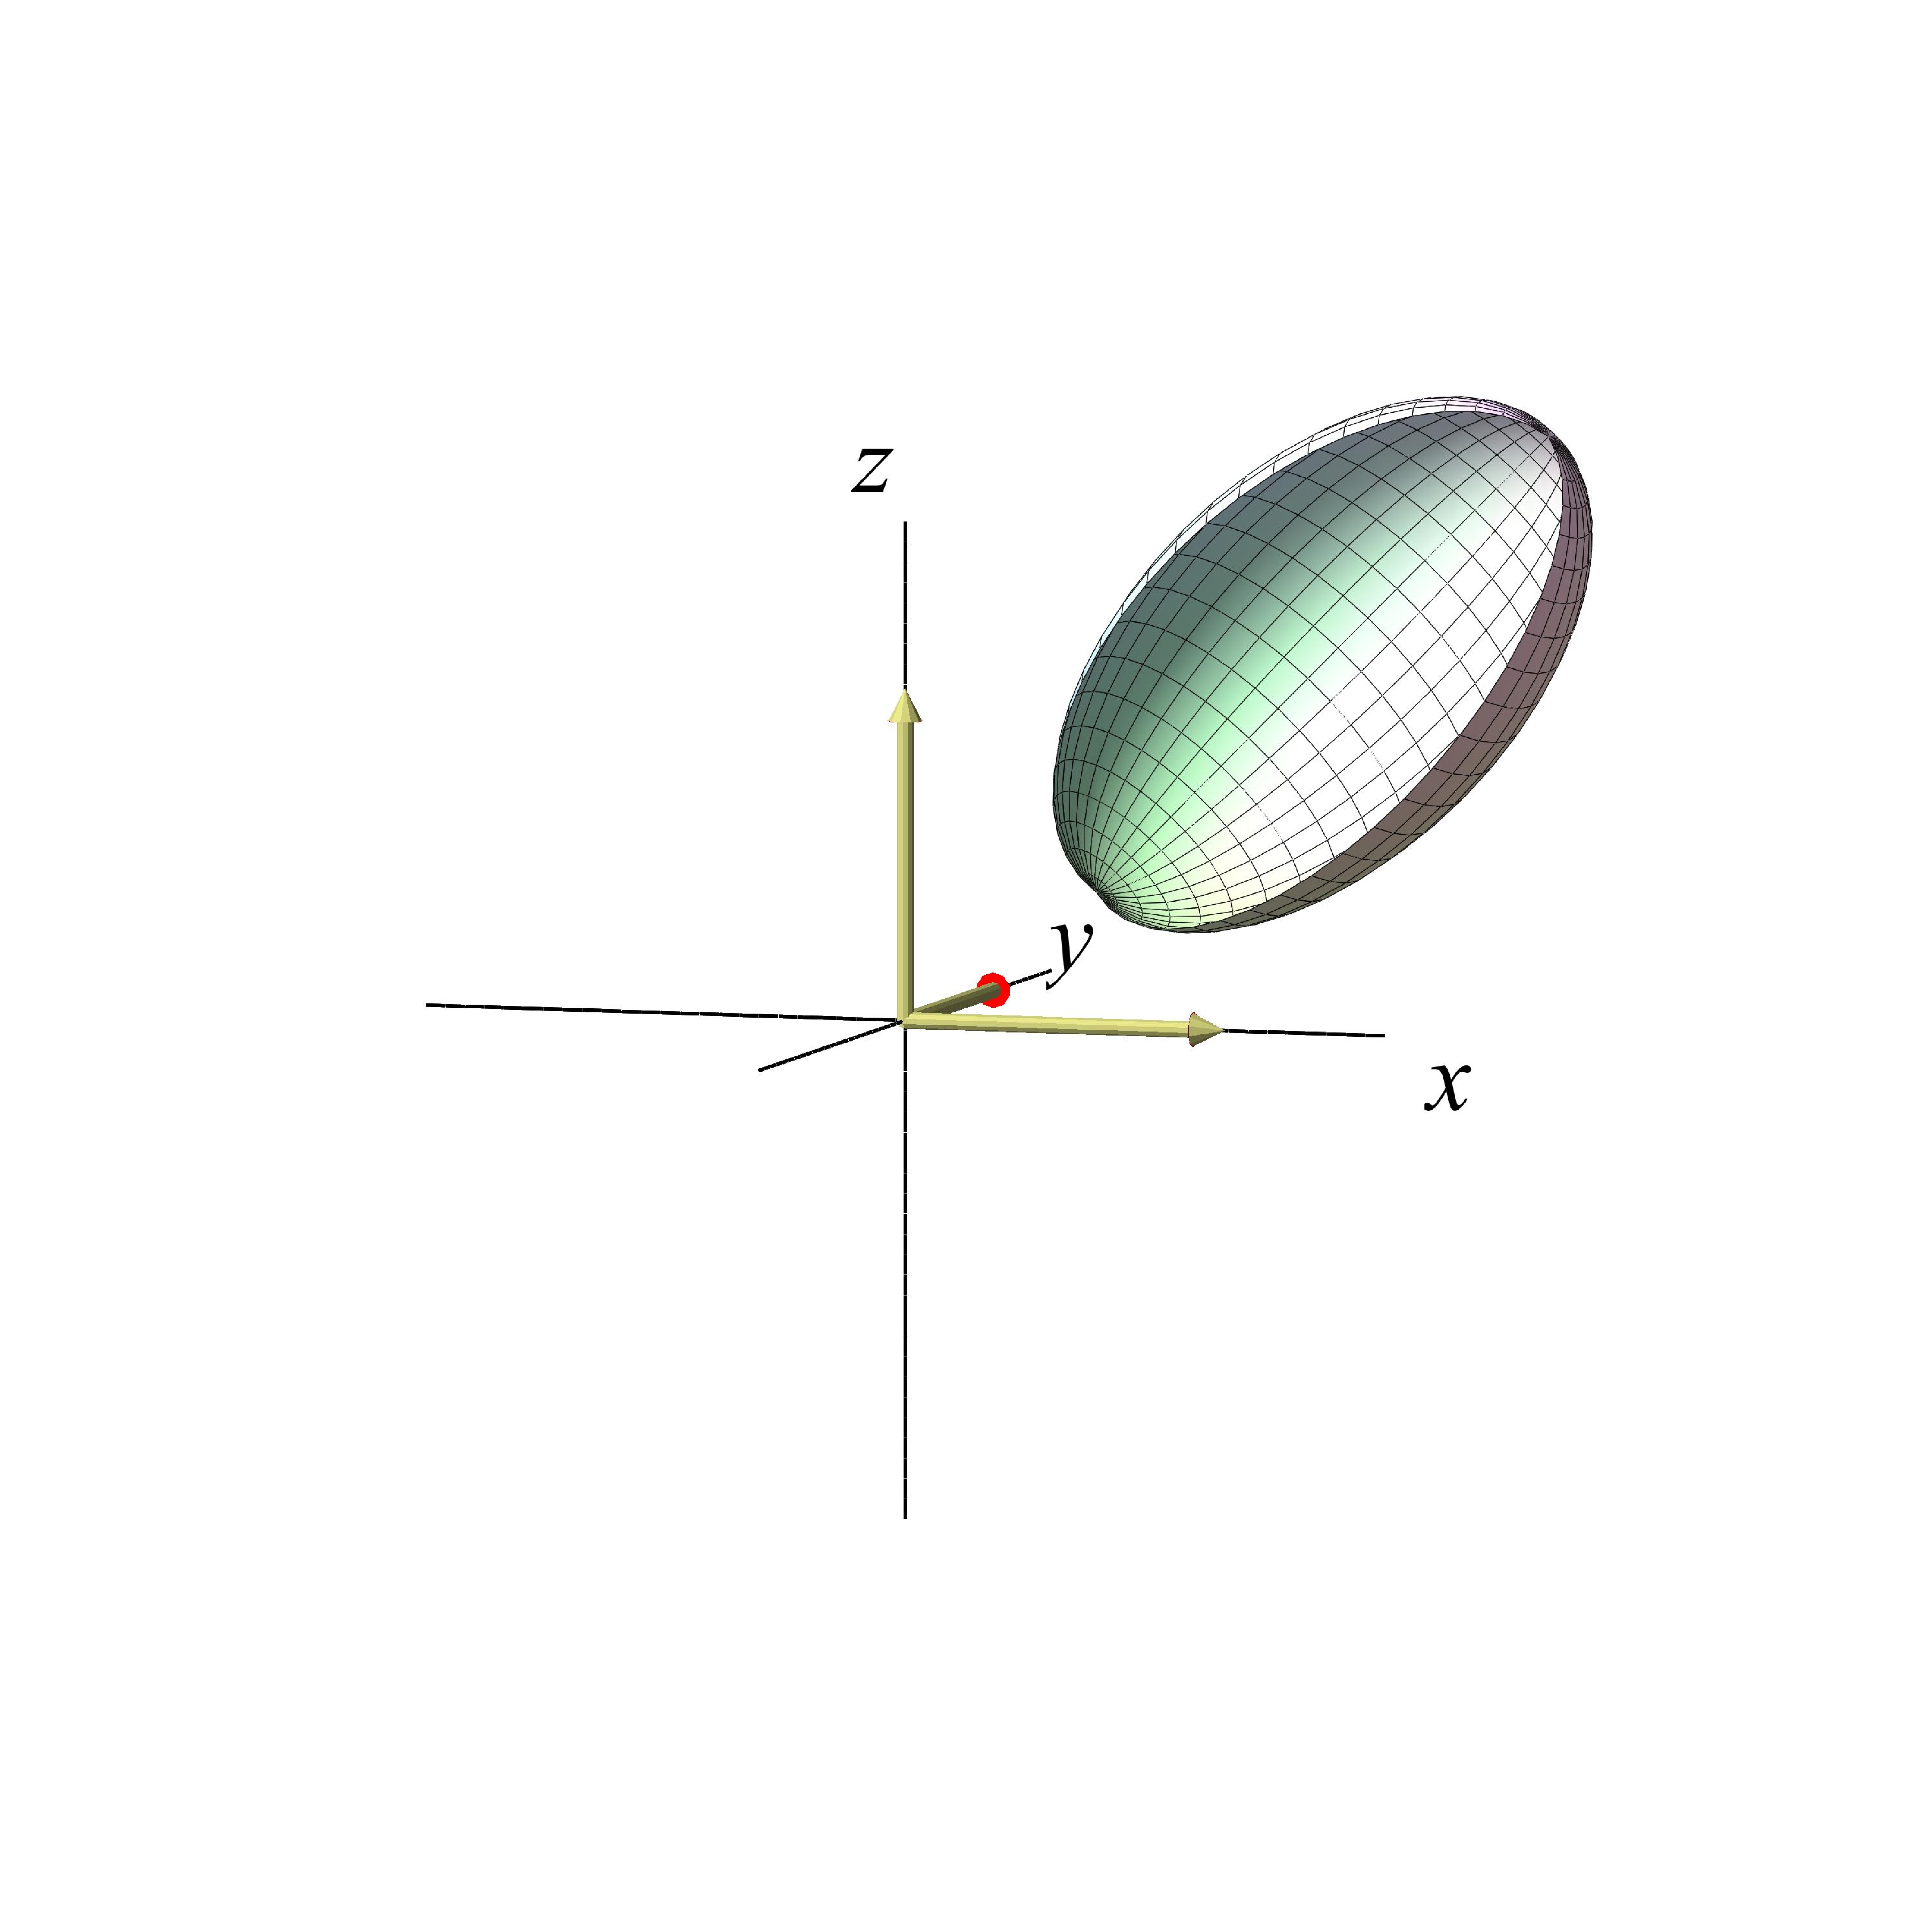
\includegraphics[height=40mm]{FIGS/plotEllConstr4.pdf}}
\begin{center}
\caption{Konstruktion af ellipsoiden fra eksempel \ref{exampEllipsoide}  ud fra data om beliggenhed, akser, og rotations\-matrix.} \label{figEllConstr}
\end{center}
\end{figure}

\begin{example}[Ellipsoidedata] \label{exampFunkEll}
Den konstruerede ellipsoide i eksempel \ref{exampEllipsoide} er $0$-niveaufladen for andengradspolynomiet med følgende data:
\begin{equation}
\begin{aligned}
f(x,y, z) &=  2\cdot x^{2} + 2\cdot y^{2} + 2\cdot z^{2} - 2\cdot x - 4\cdot y - 2 \cdot z - 2\cdot x \cdot z + 3\quad . \\   \\
\bm{\nabla}f(x,y,z) &= ( 4\cdot x - 2\cdot z -2\, , \, 4\cdot y - 4 \, , \, -2\cdot x + 4 \cdot z - 2  ) \quad . \\  \\
\frac{1}{2}\cdot \mathbf{H}f(x,y,z) &= \left[
                     \begin{array}{ccc}
                       2 & 0 & -1\\
                       0 & 2 & 0 \\
                       -1 & 0 & 2\\
                     \end{array}
                   \right] \quad . \\  \\
\bm{\Lambda} &= \left[
                     \begin{array}{ccc}
                       3 & 0 & 0 \\
                       0 & 2 & 0 \\
                       0 & 0 & 1 \\
                     \end{array}
                   \right] \quad . \\  \\
\mathbf{Q} &= \left[
                     \begin{array}{ccc}
                       - \sqrt{2}/2 & 0 & - \sqrt{2}/2 \\
                     0& 1& 0\\
                      \sqrt{2}/2 &0 & - \sqrt{2}/2\\
                     \end{array}
                   \right]\quad . \\  \\
\widetilde{f}(\widetilde{x}, \widetilde{y}, \widetilde{z}) & = 3\cdot \widetilde{x}^{2} + 2\cdot \widetilde{y}^{2} + \widetilde{z}^{2}  -4\cdot \widetilde{y}+  2\cdot\sqrt{2}\cdot \widetilde{z} +3 \\
&= 3\cdot \widetilde{x}^{2} + 2\cdot\left(\widetilde{y} - 1 \right)^{2} + \left(\widetilde{z} +\sqrt{2} \right)^{2}-1 \quad.
\end{aligned}
\end{equation}
Den andengradsligning som giver niveaufladen $\mathcal{K}_{0}(f)$ er derfor givet ved ligningen:
\begin{equation}
\left(\frac{\widetilde{x}}{\frac{1}{\sqrt{3}}}\right)^{2} + \left(\frac{\widetilde{y} - 1}{\frac{1}{\sqrt{2}}}\right)^{2} +  \left(\widetilde{z} +\sqrt{2}\right)^{2} = 1 \quad ,
\end{equation}
hvorfra vi aflæser de ovenfor givne halvakser $a =\frac{1}{\sqrt{3}}$, $b=\frac{1}{\sqrt{2}}$, og $c=1$ samt centerkoordinaterne $\vekind{v}(\mathbf{C}) = (0, 1, -\sqrt{2})$ som via substitutionsmatricen $\mathbf{Q}$ svarer til koordinaterne $\vekind{e}(\mathbf{C}) = (1,1,1)$ med hensyn til standard-basis e.
\end{example}

%%%%%%%%%%%%%%%%%%%%%%%%%%%%%%%%%%%%%%%%%%%%%%%%%%%%%%%%%%%%%
%%%%%%%%%%%%%%%%%%%%%%%%%%%%%%%%%%%%%%%%%%%%%%%%%%%%%%%%%%%%%
%%%%%%%%%%%%%%%%%%%%%%%%%%%%%%%%%%%%%%%%%%%%%%%%%%%%%%%%%%%%%




%%%%%%%%%%%%%%%%%%%%%%%%%%%%%%%%%%%%%%%%%%%%%%%%%%%%%%%%%%%%%
%%%%%%%%%%%%%%%%%%%%%%%%%%%%%%%%%%%%%%%%%%%%%%%%%%%%%%%%%%%%%
%%%%%%%%%%%%%%%%%%%%%%%%%%%%%%%%%%%%%%%%%%%%%%%%%%%%%%%%%%%%%




%%%%%%%%%%%%%%%%%%%%%%%%%%%%%%%%%%%%%%%%%%%%%%%%%%%%%%%%%%%%%
%%%%%%%%%%%%%%%%%%%%%%%%%%%%%%%%%%%%%%%%%%%%%%%%%%%%%%%%%%%%%
%%%%%%%%%%%%%%%%%%%%%%%%%%%%%%%%%%%%%%%%%%%%%%%%%%%%%%%%%%%%%

\begin{summary}
Hovedresultatet i denne eNote er en identifikation -- via en række konkrete eksempler -- af de mulige niveaukurver og -flader for andengradspolynomier i to og tre variable. Metoden er reduktionsmetoden for kvadratiske former og andengradspolynomier,  som er indført i \tref{NUID33-tn18}{eNote}. Baseret på samme metode angives en strategi til parametrisering og præsentation af de enkelte niveauflader for funktioner af tre variable.
\end{summary}


%%%%%%%%%%%%%%%%%%%%%%%%%%%%%%%%%%%%%%%%%%%%%
%%%%%%%%%%%%%%%%%%%%%%%%%%%%%%%%%%%%%%%%%%%%%
%%% HER SKAL DU STOPPE MED AT SKRIVE %%%%%%%%
%%%%%%%%%%%%%%%%%%%%%%%%%%%%%%%%%%%%%%%%%%%%%
%%%%%%%%%%%%%%%%%%%%%%%%%%%%%%%%%%%%%%%%%%%%%


\end{document} 

%%%%%%%%%%%%%%%%%%%%%%%%%%%%%%%%%%%%%%%%%%%%%%%%%%%
%%%%%%%%%%%%%%%%%%%%%%%%%%%%%%%%%%%%%%%%%%%%%%%%%%%

